\documentclass[11pt]{article}
\usepackage[margin=1in]{geometry}
\usepackage{amsmath,amssymb,amsthm,booktabs,hyperref,graphicx}
\usepackage{mathtools}
\usepackage{fancyhdr}
\pagestyle{fancy}\fancyhf{}
\fancyhead[L]{\footnotesize The Riemann Hypothesis for Generalized Petersen Graphs}
\fancyhead[R]{\footnotesize\thepage}
\renewcommand{\headrulewidth}{0.4pt}

% Every certification count and threshold below is GENERATED by
% verification/verify_all.py from the certificates on disk.  The census has
% drifted three times (54, 55, 56) and L(4) three times (31, 30, 29), always by
% a bookkeeping slip and never by a change to the theory, so these numbers are
% no longer written by hand anywhere in this paper.
% GENERATED by verification/verify_all.py -- do not edit by hand.
% Every number here is read off the certificates on disk.

\newcommand{\NtileThree}{23}
\newcommand{\LvalThree}{21}
\newcommand{\LmaxThree}{43}
\newcommand{\NtileFour}{33}
\newcommand{\LvalFour}{29}
\newcommand{\LmaxFour}{61}
\newcommand{\NtileFive}{21}
\newcommand{\LvalFive}{54}
\newcommand{\LmaxFive}{75}
\newcommand{\NtileThreeFour}{56}
\newcommand{\NtileAll}{77}
\newcommand{\SettleThree}{21}
\newcommand{\SettleFour}{29}
\newcommand{\SettleFive}{162}
\newcommand{\NcertGN}{17}
\newcommand{\GNlo}{17}
\newcommand{\GNhi}{33}
\newcommand{\MaxAlpha}{1.0\times10^{-9}}
\newcommand{\RamLastOne}{14}
\newcommand{\RamCountOne}{9}
\newcommand{\RamLastTwo}{23}
\newcommand{\RamCountTwo}{19}
\newcommand{\RamLastThree}{32}
\newcommand{\RamCountThree}{18}
\newcommand{\RamLastFour}{42}
\newcommand{\RamCountFour}{34}
\newcommand{\RamLastFive}{50}
\newcommand{\RamCountFive}{28}
\newcommand{\RamLastSix}{49}
\newcommand{\RamCountSix}{20}
\newcommand{\RamLastSeven}{70}
\newcommand{\RamCountSeven}{39}
\newcommand{\RamLastEight}{49}
\newcommand{\RamCountEight}{16}
\newcommand{\RamLastNine}{90}
\newcommand{\RamCountNine}{50}
\newcommand{\RamLastTen}{52}
\newcommand{\RamCountTen}{14}
\newcommand{\RamTotal}{247}
\newcommand{\RamKmax}{10}
\newcommand{\RamCases}{458}
\newcommand{\RamBoundTwo}{23}
\newcommand{\RamBoundThree}{32}
\newcommand{\RamBoundFour}{42}
\newcommand{\RamDirichlet}{231}
\newcommand{\RamAllTotal}{460}
\newcommand{\RamAllIso}{324}
\newcommand{\RamAllMaxN}{112}
\newcommand{\RamAllMaxK}{45}
\newcommand{\RamAllSizes}{80}
\newcommand{\RamAllCases}{13110}
\newcommand{\RatClassTwo}{7,9,15,20}
\newcommand{\RatClassThree}{10,24,42}
\newcommand{\RatClassFour}{60,70,90}
\newcommand{\RatClassFive}{24,126}
\newcommand{\RatClassSix}{\text{none}}
\newcommand{\RatClassSeven}{120}
\newcommand{\TileAllK}{9}
\newcommand{\Nchecks}{150}

\newtheorem{theorem}{Theorem}
\newtheorem{lemma}[theorem]{Lemma}
\newtheorem{corollary}[theorem]{Corollary}
\newtheorem{conjecture}[theorem]{Conjecture}
\newtheorem{proposition}[theorem]{Proposition}
\setlength{\emergencystretch}{3em}
\theoremstyle{definition}
\newtheorem{remark}[theorem]{Remark}
\newtheorem{observation}[theorem]{Observation}
\newtheorem{question}[theorem]{Question}
\newtheorem{definition}[theorem]{Definition}

\title{Where Optimal Networks Stop Existing: Certified Spectral Limits\\
of Cyclic Architectures for Quantum Controllability and Bottleneck-Free Routing}
\author{Aryan Padarthi}
\date{September 23, 2026}

\begin{document}
\maketitle

\begin{abstract}
This paper studies one family of graphs -- the generalized Petersen graphs
$P(n,k)$, and cyclic covers more generally -- with one engine, and answers two
questions about it. Both questions are about the spectrum of a matrix attached
to the graph; they differ in whether the matrix is fixed or ranges over a class.
The engine is one object, the \emph{symbol} $M(\zeta)$ of the cyclic cover: a
$2\times2$ matrix of Laurent polynomials in $\zeta$, which evaluated at the
$n$-th roots of unity gives the $n$ Fourier blocks of any rotation-invariant
matrix on $P(n,k)$. Part~I asks where the eigenvalues of $M(\zeta)$ lie as
$\zeta$ runs over the grid, for the one matrix with adjacency weights; Part~II
asks how often $\det M(\zeta)$ can vanish on the same grid when the weights are
free, and then what survives when the weights are allowed to vary around the
ring. Same grid, same symbol, two questions.

\medskip\noindent\textbf{Part I: which of these graphs satisfy the Riemann
Hypothesis.}
Attached to a finite graph is its Ihara zeta function, which has an Euler
product, a functional equation, and a prime number theorem for closed geodesics.
For a $(q+1)$-regular graph one can ask the Riemann Hypothesis for it, and by
the Ihara determinant formula the answer is equivalent to a finite spectral
condition: the graph satisfies the RH if and only if it is \emph{Ramanujan},
every eigenvalue with $|\lambda|\ne q+1$ obeying $|\lambda|\le2\sqrt q$
\cite[Ex.~9]{terras}. The analogous question has been settled for other
families: Droll classified Ramanujan unitary Cayley graphs, and Le and
Sander~\cite{lesander} classified Ramanujan integral circulant graphs of prime
power order, in both cases finding only finitely many members qualify.
Which $P(n,k)$ satisfy the Riemann Hypothesis appears not to have been asked,
although the spectrum has been completely known since~\cite{gs} --- a paper
containing no occurrence of \emph{Ramanujan}, \emph{expander} or \emph{spectral
gap}. We answer it completely, for every $n$ and every $k$.

Clearing both radicals in the eigenvalue comparison --- twice legitimately,
since $|A|\le4<4\sqrt2$ and $7+P\ge3$ make each squaring an equivalence rather
than an implication --- collapses the analytic statement to the nonnegativity of
a single integer polynomial,
\[
  D_k(u)=\bigl(7+4u\,T_k(u)\bigr)^2-8\bigl(2u+2T_k(u)\bigr)^2,
  \qquad\deg D_k=2k+2,
\]
evaluated on the grid $u=\cos(2\pi j/n)$. Since $D_k(1)=-7$, the grid must clear
a band at $u=1$, and a fine grid cannot. Monotonicity, AM--GM and
$1-\cos\theta\le\theta^2/2$ turn this into a bound holding for \emph{every} $k$,
\[
  n\ \le\ \pi\bigl(2+\sqrt2\bigr)\sqrt{k^2+1},
\]
with the sharper $n\le2\pi/\arccos u_k$ available for each individual $k$ from
the largest root $u_k$ of $D_k$ below $1$.
Since $D_k(-1)=-7$ for odd $k$ and $+9$ for even $k$, there is a second band at
$u=-1$ exactly when $k$ is odd --- but the grid meets $u=-1$ only when $n$ is
even, and there the sample is the trivial eigenvalue $-3$ of a bipartite graph,
which the Ramanujan condition exempts. Hence a \emph{parity law}: for odd $k$,
odd $n$ is cut off at \emph{exactly half} the same constant, and bipartiteness
\emph{helps}. The per-$k$ forms are sharp in cases: the first is attained at
$k=2,3,4$ and the second at $k=1,5,7,9$.

Neither bound is uniform in $k$, so neither closes the question. Two further
steps do. First, $D_k$ is a difference of squares, so it factors over
$\mathbb Q(\sqrt2)$ into the two eigenvalue conditions $f_\pm=7+P\pm2\sqrt2A$;
these cannot both be negative, since $f_-+f_+=2(7+P)\ge6$, and under
$x=\cos\frac{\pi j(k+1)}{n}$, $y=\cos\frac{\pi j(k-1)}{n}$ both collapse to the
same quadratic form
\[
  Q(x,y)=4x^{2}+4y^{2}-8\sqrt2\,|xy|+3\ \ge\ 0 ,
\]
which \emph{does not involve $k$}. The forbidden set is one fixed region --- four
congruent pieces at the corners of the square, each of area
$\tfrac32-\sqrt2+\tfrac38\log\frac{1+\sqrt2}{3}$, together $0.4322\%$ of it ---
and $k$ survives only in the map into the square. Second, failure is forced
whenever $\|j/n\|^{2}+\|jk/n\|^{2}<\tau/2\pi^{2}$, a \emph{simultaneous
Diophantine} condition, and Dirichlet's approximation theorem supplies such a
$j$ unconditionally: with $J=\lfloor\sqrt n\rfloor$ some $j\le J$ has
$\|jk/n\|\le1/(J+1)$, making the left side less than $2/n$. Hence
$n\ge\RamDirichlet$ fails for \emph{every} $k$, and since $1\le k<n/2$ the family
is finite in both variables.

What remains is finite and is certified in exact arithmetic, never floating
point: on the grid $A=c_1+c_k$ and $P=c_{k+1}+c_{k-1}$ are values of integer
Laurent polynomials at roots of unity, so reduction modulo $\Phi_m$ decides
band-edge vanishing by integer arithmetic, and a separation bound for nonzero
algebraic integers guards every sign. Exhausting the region gives the
classification outright: exactly $\RamAllTotal$ pairs $(n,k)$ satisfy the
Riemann Hypothesis, $\RamAllIso$ graphs up to isomorphism, from $\RamAllCases$
cases each decided exactly; the largest is $n=\RamAllMaxN$, and no $P(n,k)$ with
$k>\RamAllMaxK$ qualifies at all. The
classification is not monotone in $k$ --- $k=9$ reaches $n=\RamLastNine$ while
$k=8$ and $k=10$ stop at $\RamLastEight$ and $\RamLastTen$ --- because for even
$k$ an interior band binds first; the same asymmetry closes the list, since past
$k=25$ no even $k$ survives at all.

None of this used $P(n,k)$ beyond ``two-vertex base, cubic cover''. There are
exactly two such bases, and the criterion carries to both: the two-loop base
$B(a,b,c)$ by the \emph{same} $Q$ with $(a+b,a-b)$ in place of $(k+1,k-1)$, the
edge voltage $c$ playing no role at all, and the theta base by
$\sum_{l<m}\cos\frac{2\pi j(c_l-c_m)}{n}\le\frac52$. For a base of any size,
$M_1\to M_0$ as $n\to\infty$ and $M_0$ has top eigenvalue $3$, so some
nontrivial eigenvalue exceeds $2\sqrt2$: \emph{no infinite family of Ramanujan
graphs is a cyclic cover of a fixed base}. That is the cyclic instance of the
known principle that abelian covers do not expand, made explicit with a
constant. Finally the \emph{deficit} $\delta=\lambda_2-2\sqrt2$ measures what
the no-go costs, and is bounded by $3-2\sqrt2$ throughout.

\medskip\noindent\textbf{Part II: how degenerate the zero eigenvalue can be,
over every matrix carrying the pattern.}
Over all symmetric matrices whose off-diagonal support is exactly $E(G)$ ---
Hamiltonians on that network --- how degenerate can the zero eigenvalue be? That
maximum, the maximum nullity $M(G)$, is the central quantity of the inverse
eigenvalue problem of a graph, and determining it exactly is a statement about
\emph{every} matrix carrying the pattern. It is bounded by the zero forcing
number, $M(G)\le Z(G)$, so a matrix of large nullity and a small forcing set
together pin down both.

We study them for \emph{cyclic covers}: given a base graph $B$
with edge voltages in $\mathbb Z_n$, the derived graph $B^n$ on
$V(B)\times\mathbb Z_n$. This is the setting of discrete Floquet theory, and the
difficulty is that an answer must hold uniformly in the period $n$.
Generalized Petersen graphs are the case of a
two-vertex base with voltages $1$, $k$ and $0$.

Our main structural result is that for such a cover the nullity is governed by
a single scalar object determined by the voltages. For $P(n,k)$ we prove it for
\emph{every} matrix carrying the pattern, symmetric or not: eliminating the
inner coordinates leaves one nine-term linear recurrence of order $2k+2$, so
\[
  \operatorname{null}A=\dim\ker(T-I)\le 2k+2,
\]
$T$ the monodromy, with equality iff $T=I$. The order $2k+2$ is exactly the
size of the forcing set produced by a rotation-bootstrap argument that gives
$Z(P(n,k))\le2k+2$, so \emph{the ceiling of the matrix-certificate method
coincides with the upper bound it is trying to match}: either the method settles
$Z$ completely or nothing does. For a general cover the same reduction holds for
equivariant matrices, with the ceiling given by the degree span of
$\det M(\zeta)$; and whenever the top coefficient of $\det M(\zeta)$ is a
monomial in the edge weights, the ceiling holds for \emph{every} matrix carrying
the pattern of the cover, the kernel of the lifted operator on the infinite
strip having dimension exactly the span (Theorem~\ref{thm:leading}).

We then reach the ceiling. Under the rotation the singularity condition is a
monic degree-$(k+1)$ polynomial in $s=2\cos(2\pi m/n)$ carrying exactly three
free parameters for every $k$; three roots may be prescribed and no more, but a
symbol with rational coefficients drags its whole Galois orbit onto the grid
$\{2\cos(2\pi m/n)\}$. Choosing the symbol to be a product of minimal
polynomials of $2\cos(2\pi/d)$ yields explicit \emph{integer} certificates and
hence
\[
  Z(P(n,4))=M(P(n,4))=10,\qquad Z(P(n,5))=M(P(n,5))=12,
\]
for every $n$ divisible by $60$, $70$ or $90$, respectively by $24$. For
$k\ge4$ the only exact values previously known are $Z(P(2k+1,k))=6$
\cite[Thm.~2.6]{RST}, a single $n$ for each $k$ at which the bound $2k+2$ is far
from attained; these are the first at which it is \emph{attained}, and the first
holding for infinitely many $n$. In the second case the certificate is the adjacency matrix
itself, and we classify its nullity completely: with
$P_k(z)=z^{2k+2}+z^{2k}-z^{k+1}+z^2+1$,
$\operatorname{null}(\mathrm{Adj}\,P(n,k))=\sum\varphi(d)$ over those $d$ with
$\Phi_d\mid P_k$ and $d\mid n$, a Conway--Jones phenomenon; in particular the
adjacency matrix is never singular for $k=3,6,9$.

Against this we prove a matching \emph{obstruction}. Realisability of a
certificate is the positivity (or nonvanishing) of $c^{2}=a\alpha-\beta$, and
because $L_k(-s)=(-1)^{k}L_k(s)$, for \emph{every even} $k$ a symbol with two
roots $y,-y$ has $c^{2}=0$ identically, while for odd $k$ no such obstruction
exists. For $k=2$, where the symbol has three roots and no residual conditions,
this is the whole story in closed form:
\[
  c^{2}=-(s_1+s_2)(s_1+s_3)(s_2+s_3),
\]
so the construction fails precisely when two prescribed roots are antipodal.
Counting antipodal classes on the grid then settles $k=2$ for all $n$:
$Z(P(n,2))=M(P(n,2))=6$ for every $n\ge9$ with $n\ne10$, by an explicit
certificate at the three most negative grid values. The rational symbol
$\Psi_7$ has $c^{2}=-1$, so \emph{that symbol} admits no symmetric certificate,
while an integer non-symmetric matrix of nullity $6$ exists for every $n$
divisible by $7$; since the main branch already covers $n\ge9$, $n\ne10$, the
one value where the larger matrix class is needed rather than merely available
is $n=7$.
The two exceptions are of opposite kinds --- $Z(P(8,2))=5$, so there the method
is right to fail, and $Z(P(10,2))=6$, so there it is the method that falls
short.

The same analysis is what settles the remaining cases, because only $c^{2}=0$
is fatal: a symbol with $c^{2}<0$ admits no symmetric certificate but is
realisable once the two spoke weights are allowed to differ. Redoing our
exhaustive enumeration of rational symbols under the weaker condition turns two
cases we had recorded as impossible into exact values. Both come from the
\emph{signed} adjacency matrix, the adjacency matrix of $P(n,k)$ with one set of
spokes negated, whose nullity we classify by the polynomial
$Q_k(z)=z^{2k+2}+z^{2k}+z^{k+1}+z^{2}+1$ --- the unsigned $P_k$ with the middle
sign reversed. $Q_k$ splits into cyclotomics only for $k=2,3,7$ in $2\le k\le60$,
and at $k=3,7$ it gives the ceiling:
\[
  Z(P(n,3))=8\ \ (10\mid n),\qquad Z(P(n,7))=16\ \ (120\mid n),
\]
by matrices of zeros and $\pm1$, the second replacing a floating-point claim by
an exact one. Conversely $k=6,8,9,10$ are \emph{impossible} over $\mathbb Q$ in
both classes, and now for an identified reason: every candidate clearing the
family condition is one of at most $25$ degenerate symbols, the bound coming
from Niven's theorem.

Breaking the symmetry to period $d$, the map from weights to the coefficients of
the symbol has rank $\min(2d+1,k+1)$ in every case computed, so every symbol
becomes reachable exactly when $d\ge\lceil k/2\rceil$. This yields
$Z(P(n,6))=14$ at $n=60,72,84,90,96,108,120$, $Z(P(96,7))=16$ and
$Z(P(96,8))=18$, though these certificates are verified numerically rather than
in exact arithmetic. Every exact value above holds for $n$ in a divisibility class, and we prove that
this is forced: a period-one symbol is a fixed polynomial, its roots are fixed
algebraic numbers, and a fixed algebraic number lies on $\Gamma_n$ only for $n$
in one divisibility class --- which contains at most one prime. For $k\ge3$ an
$n$-dependent choice of roots is constrained by the identity $e_2=-k$, a
Conway--Jones relation on the grid; for $k=2$ that condition is vacuous, which is
exactly why $k=2$ is general in $n$ and no other $k$ is.

Escaping this needs the non-invariant matrices, and the ceiling corollary
supplies the criterion: $\operatorname{null}A=2k+2$ if and only if the monodromy
is the identity, a condition with no arithmetic in it. We certify that condition
rigorously, not numerically, by recasting it as the bilinear system $A(w)K(X)=0$
with $K$ in graph form and applying a Krawczyk contraction test; the square
subsystem must be chosen structurally, since $K^{\!\top}\!AK$ is symmetric and
its antisymmetric part accounts for exactly $\binom{2k+2}2$ dependencies. This
gives $Z(P(n,3))=M(P(n,3))=8$ at $n=17,19,21,23,25,27$, the primes $17,19,23$
among them --- values that no period-one certificate can reach, and the first in
this paper not lying on a congruence class. Finally we obtain a statement for \emph{all}
large $n$. Tiles carrying a fixed docking pattern at both ends have transfer
products depending only on their interiors, so identity tiles of every length in
$[L,2L)$ give $Z(P(n,k))=2k+2$ for every $n\ge L$ --- a finite list of finite
problems. The existence of those tiles is the one computer-assisted step in
this paper, and it is exact: every bound in the contraction test is a rational
number and the final inequality an integer comparison, so the step is a proof
in the sense of the four-colour and Kepler proofs, not a numerical observation.
Separately, and without finding any tile, an elliptic choice of dock and a
single full-rank evaluation of the tile differential imply that identity tiles
of \emph{every} sufficiently large length exist (Theorem~\ref{thm:tilesallk},
hypotheses certified exactly for $k\le\TileAllK$), and the rank condition is proved for every $k$ by a second-order argument in
$\mathfrak{sp}(2k+2)$ (\S\ref{sec:tilesrank}); together these give
$Z(P(n,k))=M(P(n,k))=2k+2$ for all sufficiently large $n$, \emph{for every}
$k\ge2$, with an ineffective threshold. Carrying the explicit construction out and verifying all $\NtileAll$ tiles involved,
\[
  Z(P(n,3))=M(P(n,3))=8\ \ (n\ge17),\qquad
  Z(P(n,4))=M(P(n,4))=10\ \ (n\ge\SettleFour),
\]
\[
  Z(P(n,5))=M(P(n,5))=12\ \ (n\ge\SettleFive),
\]
with no congruence condition. Together with exhaustive search on the finitely
many smaller $n$, this determines $Z(P(n,k))$ for \emph{every} $n$ when $k=2$,
$k=3$ and $k=4$ --- the last two for the first time, since the previously
published value for $k=3$ is false and no value at all was known for $k=4$. In particular $Z(P(n,3))=8$ for every $n\ge13$, and $13$ is optimal since
$Z(P(11,3))=Z(P(12,3))=7$; four exhaustive searches at $n=13,\dots,16$ close the
gap below the tiling range. This proves \emph{Conjecture 5} of~\cite{K}, whose
stated missing ingredient --- ``a lower-bound proof valid for all large $n$'' ---
is precisely what the tiling construction supplies, and fixes at $13$ the
stabilization threshold that note leaves open. The tile condition is a rational equation, but
certifying it needs no interval arithmetic on rational maps: by the ceiling
corollary the monodromy of the one-tile cyclic matrix \emph{is} the tile product,
so the same bilinear system certifies it.

We state throughout which claims are proved, which rest on exact certificates,
which on interval certification, which are numerical, and which earlier claims of
ours are corrected or withdrawn.
\end{abstract}

% ---------------------------------------------------------------------------
% MAIN RESULTS -- assembled summary. The statements below are lifted verbatim
% from the theorems they cite; no claim is made here that is not proved there.
% ---------------------------------------------------------------------------
\section*{Main results}

\noindent\textbf{Part I --- which $P(n,k)$ satisfy the Riemann Hypothesis}
(for the Ihara zeta function; equivalently, which are Ramanujan).

\begin{enumerate}\setlength{\itemsep}{2pt}
\item[(I.1)] If $P(n,k)$ satisfies the Riemann Hypothesis then
  $n\le\pi(2+\sqrt2)\sqrt{k^2+1}$, and if $k$ and $n$ are both odd,
  $n\le\tfrac12\pi(2+\sqrt2)\sqrt{k^2+1}$. \hfill (Theorem~\ref{thm:uniform})
\item[(I.2)] \emph{Parity law.} For odd $k$ and odd $n$,
  $n\le\pi/\arccos(-v_k)$; no such restriction for even $n$ or even $k$.
  \hfill (Theorem~\ref{thm:parity})
\item[(I.3)] Exactly $\RamAllTotal$ pairs $(n,k)$ qualify, in $\RamAllIso$
  isomorphism classes; no $k>\RamAllMaxK$ occurs. All $\RamAllCases$ cases
  decided in exact arithmetic. \hfill (Theorem~\ref{thm:allk})
\end{enumerate}

\medskip\noindent\textbf{Part II --- maximum nullity and zero forcing.}

\begin{enumerate}\setlength{\itemsep}{2pt}
\item[(II.1)] \emph{Ceiling.} For every matrix carrying the $P(n,k)$ pattern,
  symmetric or not, $\operatorname{null}A=\dim\ker(T-I)\le2k+2$, with equality
  iff $T=I$. \hfill (Theorem~\ref{thm:red})
\item[(II.2)] $Z(P(n,k))$ is determined for \emph{every} admissible $n$ when
  $k=2$, $k=3$ and $k=4$. \hfill (Theorem~\ref{thm:complete})
\item[(II.3)] $Z(P(n,3))=8$ for every $n\ge13$, and $13$ is optimal --- this is
  Conjecture~5 of~\cite{K}. \hfill (Theorem~\ref{thm:k3krishnan})
\item[(II.4)] $Z(P(n,k))=M(P(n,k))=2k+2$ for all sufficiently large $n$, for
  every $2\le k\le\TileAllK$; the threshold is ineffective.
  \hfill (Proposition~\ref{prop:tilesallk})
\end{enumerate}

\medskip\noindent
Section~\ref{sec:contribution} states what these do and do not contribute, and
the Status of the claims section labels every claim by the standard it meets.

\part{The Riemann Hypothesis for Generalized Petersen Graphs}
\label{part:rh}

\section{The graph Riemann Hypothesis}\label{sec:grh}

Attached to a finite connected graph $X$ is its \emph{Ihara zeta function},
\[
  \zeta_X(u)=\prod_{[C]}\bigl(1-u^{\,\ell(C)}\bigr)^{-1},
\]
the product running over equivalence classes of primitive backtrackless
tailless closed paths, $\ell(C)$ the length. It is a graph-theoretic analogue
of the Riemann zeta function: it has an Euler product, a meromorphic
continuation, a functional equation, and a prime number theorem counting closed
geodesics. For a $(q+1)$-regular graph the substitution $u=q^{-s}$ makes the
analogy exact, and one may ask the corresponding question.

\begin{definition}[Riemann Hypothesis for a graph]
A $(q+1)$-regular graph $X$ satisfies the Riemann Hypothesis if
$\zeta_X(q^{-s})$ has no poles with $0<\mathrm{Re}\,s<1$ other than on the line
$\mathrm{Re}\,s=\tfrac12$.
\end{definition}

The point of the definition is the following equivalence, which converts an
analytic statement about a zeta function into a finite spectral one. It is
classical, following from the Ihara determinant formula; we take the statement
from Terras~\cite[Exercise 9]{terras}, where it appears in exactly this form.

\begin{theorem}[Ihara determinant formula; see \cite{terras}]\label{thm:grh}
A connected $(q+1)$-regular graph $X$ satisfies the Riemann Hypothesis if and
only if $X$ is \emph{Ramanujan}: every eigenvalue $\lambda$ of the adjacency
matrix with $|\lambda|\ne q+1$ satisfies $|\lambda|\le 2\sqrt q$.
\end{theorem}

The term is due to Lubotzky, Phillips and Sarnak~\cite{lps}, and the bound is
the best possible: $2\sqrt q$ is the spectral radius of the adjacency operator
on the universal covering tree, so a Ramanujan graph is one whose nontrivial
spectrum is as small as an infinite family can have it. Ramanujan graphs are
optimal expanders, which is why they matter outside spectral graph theory --
for communication networks, error-correcting codes, and derandomization.

Our graphs are cubic, $q+1=3$, so the threshold is
\[
  2\sqrt2 = 2.8284271247\ldots,
\]
and the trivial eigenvalues are $3$, always, and $-3$, exactly when the graph is
bipartite. We ask which generalized Petersen graphs are on the right side of it.

\begin{question}\label{q:main}
For which $n$ and $k$ does $P(n,k)$ satisfy the Riemann Hypothesis?
\end{question}

This is a natural question of a recognised kind. The analogue has been settled
for other families: Droll classified the Ramanujan unitary Cayley graphs, and
Le and Sander~\cite{lesander} classified the Ramanujan integral circulant
graphs of prime power order, in both cases finding that only finitely many
members qualify. For generalized Petersen graphs the spectrum has been
completely known since Gera and St\u{a}nic\u{a}~\cite{gs}, but we have not found
Question~\ref{q:main} raised anywhere: \cite{gs} itself contains no occurrence
of the words \emph{Ramanujan}, \emph{expander} or \emph{spectral gap}.

We answer it completely, for every $n$ and every $k$, in exact arithmetic. The
answer has four parts: a criterion reducing the question to the sign of one
integer polynomial; a change of variable after which the criterion is one fixed
region not depending on $k$; a Diophantine argument bounding $n$ uniformly in
$k$, so that the family is finite in both variables; and an exhaustive
certification of the finitely many survivors.

\section{The spectrum, and a criterion with no radicals}\label{sec:crit}

$P(n,k)$ is the cyclic cover of the two-vertex base of \S\ref{sec:covers} --
the same object this paper studies throughout -- and the block decomposition
used there is, on the zeta side, precisely the factorization of $\zeta_{P(n,k)}$
into Artin--Ihara $L$-functions over the characters of $\mathbb Z_n$. The
spectral form we need is the following, which is Theorem 2.4 of~\cite{gs}.

\begin{lemma}\label{lem:blocks}
The adjacency matrix of $P(n,k)$ is unitarily equivalent to
$\bigoplus_{j=0}^{n-1}M_j$, where
\[
  M_j=\begin{pmatrix}\alpha_j&1\\1&\beta_j\end{pmatrix},\qquad
  \alpha_j=2\cos\tfrac{2\pi j}{n},\qquad
  \beta_j=2\cos\tfrac{2\pi jk}{n}=2T_k(\alpha_j/2),
\]
with $T_k$ the Chebyshev polynomial of the first kind.
\end{lemma}

\begin{proof}
The rotation $\rho:i\mapsto i+1$ acts on $P(n,k)$ with the adjacency matrix in
its commutant, so the matrix decomposes over the characters
$\chi_j(a)=\zeta_n^{ja}$ of $\mathbb Z_n$. On the $\chi_j$ isotypic component
the outer cycle contributes $\zeta_n^{j}+\zeta_n^{-j}=\alpha_j$, the inner
$k$-step cycle contributes $\zeta_n^{jk}+\zeta_n^{-jk}=\beta_j$, and the spoke
contributes $1$ off the diagonal. The identity
$2\cos k\theta=2T_k(\cos\theta)$ gives the stated form of $\beta_j$.
\end{proof}

Deciding Question~\ref{q:main} directly from Lemma~\ref{lem:blocks} means
comparing $\bigl(\alpha+\beta\pm\sqrt{(\alpha-\beta)^2+4}\bigr)/2$ against
$2\sqrt2$ -- two nested irrationalities, and the comparison is decided at a band
edge where floating point is worth nothing. Both radicals can be cleared at
once, and what remains is a single polynomial with integer coefficients.

\begin{theorem}[Criterion]\label{thm:crit}
For $k\ge1$ define
\[
  D_k(u)=\bigl(7+4u\,T_k(u)\bigr)^2-8\bigl(2u+2T_k(u)\bigr)^2\ \in\ \mathbb Z[u],
  \qquad \deg D_k=2k+2 .
\]
Then both eigenvalues of $M_j$ lie in $[-2\sqrt2,2\sqrt2]$ if and only if
$D_k(u_j)\ge0$, where $u_j=\cos\frac{2\pi j}{n}$. The polynomial has degree
$2k+2$ and leading coefficient $4^{\,k+1}$.
\end{theorem}

\begin{proof}
Write $\alpha=\alpha_j$, $\beta=\beta_j$, $A=\alpha+\beta$, $P=\alpha\beta$.
The characteristic polynomial of $M_j$ is $\lambda^2-A\lambda+(P-1)$, with roots
$\lambda_\pm=\bigl(A\pm\sqrt{(\alpha-\beta)^2+4}\bigr)/2$.

For the upper constraint, $\lambda_+\le2\sqrt2$ is
$\sqrt{(\alpha-\beta)^2+4}\le4\sqrt2-A$. Since $|\alpha|,|\beta|\le2$ we have
$|A|\le4<4\sqrt2$, so the right-hand side is positive and squaring is an
equivalence, not merely an implication:
\[
  (\alpha-\beta)^2+4\ \le\ 32-8\sqrt2\,A+A^2 .
\]
Because $A^2-(\alpha-\beta)^2=4P$, this simplifies to $4\le32-8\sqrt2A+4P$,
that is $2\sqrt2\,A-P\le7$. Symmetrically $\lambda_-\ge-2\sqrt2$ is equivalent
to $-2\sqrt2\,A-P\le7$. The two together say
\[
  2\sqrt2\,|A|\ \le\ 7+P .
\]
Now $|P|=|\alpha\beta|\le4$, so $7+P\ge3>0$: the right-hand side is again
positive, so squaring is again an equivalence, giving $8A^2\le(7+P)^2$. Finally
$\alpha=2u$ and $\beta=2T_k(u)$, so $A=2u+2T_k(u)$ and $P=4u\,T_k(u)$, and
$(7+P)^2-8A^2=D_k(u)$.

For the degree: $T_k$ has degree $k$ and leading coefficient $2^{k-1}$, so
$\bigl(7+4uT_k\bigr)^2$ has degree $2k+2$ with leading coefficient
$\bigl(4\cdot2^{k-1}\bigr)^2=4^{\,k+1}$, while $8\bigl(2u+2T_k\bigr)^2$ has
degree only $2k$. Nothing cancels, so $\deg D_k=2k+2$ with leading coefficient
$4^{\,k+1}$.
\end{proof}

\begin{corollary}[Ramanujan, polynomially]\label{cor:crit}
$P(n,k)$ satisfies the Riemann Hypothesis if and only if
\[
  D_k\!\left(\cos\tfrac{2\pi j}{n}\right)\ \ge\ 0
  \qquad\text{for every }j\in\{1,\dots,n-1\}\text{ with }2j\ne n\text{ or }k
  \text{ even.}
\]
\end{corollary}

\begin{proof}
$P(n,k)$ is connected -- the outer cycle is connected and every inner vertex
carries a spoke -- and cubic, so by Theorem~\ref{thm:grh} the question is
whether every eigenvalue of modulus $\ne3$ has modulus $\le2\sqrt2$. By
Lemma~\ref{lem:blocks} the spectrum is $\bigcup_j\mathrm{spec}(M_j)$.

The block $M_0$ has $\alpha=\beta=2$, hence eigenvalues $3$ and $1$. If $n$ is
even and $k$ odd then $P(n,k)$ is bipartite and $M_{n/2}$ has
$\alpha=\beta=-2$, hence eigenvalues $-1$ and $-3$. No other block has $\pm3$
as an eigenvalue, since $3$ and $-3$ have multiplicity one in a connected
$3$-regular graph (and $-3$ occurs only in the bipartite case). So the two
excluded indices contribute the trivial eigenvalues together with $1$ and $-1$
respectively, both of modulus $1\le2\sqrt2$; every other index contributes only
nontrivial eigenvalues. Apply Theorem~\ref{thm:crit} at each of those.
\end{proof}

The reduction is worth pausing on. The side condition $7+P\ge0$ that licensed
the second squaring is \emph{never} binding, since $|4u\,T_k(u)|\le4$ on
$[-1,1]$ forces $7+4uT_k(u)\ge3$. So the entire Riemann Hypothesis for
$P(n,k)$ -- an analytic statement about the poles of a zeta function -- has
become the assertion that one integer polynomial is nonnegative at $n-1$
cyclotomic points. That is a statement our exact machinery can certify
outright, and \S\ref{sec:ramcert} does.

\section{The criterion without \texorpdfstring{$k$}{k}}\label{sec:corner}

Theorem~\ref{thm:crit} gives one polynomial per $k$, of degree growing with
$k$. There is a change of variable after which $k$ leaves the geometry
entirely, and what is left is a single fixed region that does not depend on
$k$ at all.

\begin{theorem}[Corner criterion]\label{thm:corner}
Put
\[
  x=\cos\frac{\pi j(k+1)}{n},\qquad
  y=\cos\frac{\pi j(k-1)}{n},\qquad
  Q(x,y)=4x^{2}+4y^{2}-8\sqrt2\,|xy|+3 .
\]
Both eigenvalues of $M_j$ lie in $[-2\sqrt2,2\sqrt2]$ if and only if
$Q(x,y)\ge0$. Hence $P(n,k)$ satisfies the Riemann Hypothesis if and only if
$Q(x,y)\ge0$ at every nontrivial index. The form $Q$ does not involve $k$.
\end{theorem}

\begin{proof}
$D_k=(7+P)^{2}-8A^{2}$ is a difference of squares, so over $\mathbb Q(\sqrt2)$
it factors as $D_k=f_-f_+$ with
\[
  f_\pm=7+P\pm2\sqrt2\,A ,
\]
each of degree $k+1$ in $u$. These factors are not new objects: the proof of
Theorem~\ref{thm:crit} produced exactly them, $f_-\ge0$ being
$\lambda_+\le2\sqrt2$ and $f_+\ge0$ being $\lambda_-\ge-2\sqrt2$. What is
required is that \emph{both} be nonnegative. They cannot both be negative,
since
\[
  f_-+f_+=2(7+P)\ge6>0
\]
by $|P|\le4$; so the product is nonnegative exactly when both factors are,
which is why the single inequality $D_k\ge0$ was equivalent to the pair.

Now set $t=2\pi j/n$, so $u=\cos t$ and $x=\cos\frac{(k+1)t}{2}$,
$y=\cos\frac{(k-1)t}{2}$. From $2\cos t\cos kt=\cos(k+1)t+\cos(k-1)t$ and
$\cos(k\pm1)t=2\cos^{2}\frac{(k\pm1)t}{2}-1$,
\[
  P=4\cos t\cos kt=2\bigl((2x^{2}-1)+(2y^{2}-1)\bigr)=4x^{2}+4y^{2}-4 ,
\]
and from $\cos t+\cos kt=2\cos\frac{(k+1)t}{2}\cos\frac{(k-1)t}{2}$,
\[
  A=2(\cos t+\cos kt)=4xy .
\]
Hence $7+P=3+4x^{2}+4y^{2}$ and
\[
  f_\mp=3+4x^{2}+4y^{2}\mp8\sqrt2\,xy ,
\]
whose minimum over the two signs is $4x^{2}+4y^{2}-8\sqrt2\,|xy|+3=Q(x,y)$.
Both are nonnegative exactly when $Q\ge0$.
\end{proof}

The content of the theorem is that $k$ has moved out of the region and into the
map. For every $k$ the question is asked about the same subset of the square.

\begin{corollary}[The forbidden set]\label{cor:lens}
\[
  Q=4\bigl(|x|-(\sqrt2+1)|y|\bigr)\bigl(|x|-(\sqrt2-1)|y|\bigr)+3 ,
\]
so $\{Q<0\}$ is bounded by a hyperbola with asymptotes
$|x|=(\sqrt2\pm1)|y|$. Its intersection with the square $[-1,1]^{2}$ is four
congruent regions, one at each corner $(\pm1,\pm1)$, each meeting the two
sides through its corner in segments of length exactly $\tfrac32-\sqrt2$ and
having area
\[
  \tfrac32-\sqrt2+\tfrac38\log\frac{1+\sqrt2}{3}=0.004321924508\ldots,
\]
so the four together occupy $0.4322\%$ of the square.
\end{corollary}

\begin{proof}
The factorisation is an expansion. The quadratic form $4x^{2}+4y^{2}-8\sqrt2xy$
has matrix of determinant $16-32<0$, so it is indefinite and the conic
$Q=0$ is a hyperbola; $\{Q<0\}$ is therefore \emph{unbounded} in the plane,
running out along the diagonals, and it is the square that cuts it into four
pieces. In the first quadrant $Q<0$ reads
$4y^{2}-8\sqrt2xy+(4x^{2}+3)<0$, i.e.\ $y$ strictly between
$y_\pm(x)=\sqrt2x\pm\tfrac12\sqrt{4x^{2}-3}$. Now $y_+(x)>1$ throughout
$[\tfrac{\sqrt3}{2},1]$, since $y_+(x)=1$ would force $\sqrt2x\le1$; and
$y_-(x)\le1$ exactly when $x^{2}-2\sqrt2x+\tfrac74\le0$, i.e.\ $x\ge\sqrt2-\tfrac12$.
So inside the square the region is
$\{\sqrt2-\tfrac12\le x\le1,\ y_-(x)\le y\le1\}$, which meets the side $y=1$
in a segment of length $1-(\sqrt2-\tfrac12)=\tfrac32-\sqrt2$, and by the
symmetry of $Q$ likewise on $x=1$. Its area is
$\int_{\sqrt2-1/2}^{1}\bigl(1-y_-(x)\bigr)\,dx$, which evaluates to the stated
closed form.
\end{proof}

Figure~\ref{fig:corner} is the criterion: the square, the four regions, and the
$n-1$ image points. It also makes the parity law of
Theorem~\ref{thm:parity} visible. When $n$ is even and $k$ odd the excluded
index $j=n/2$ lands on the corner $(-1,+1)$ --- inside a forbidden region ---
and is forgiven, because the eigenvalue it carries is the trivial $-3$ of a
bipartite graph. The exemption of one point is the whole of the parity law.

\begin{figure}[h]
\centering
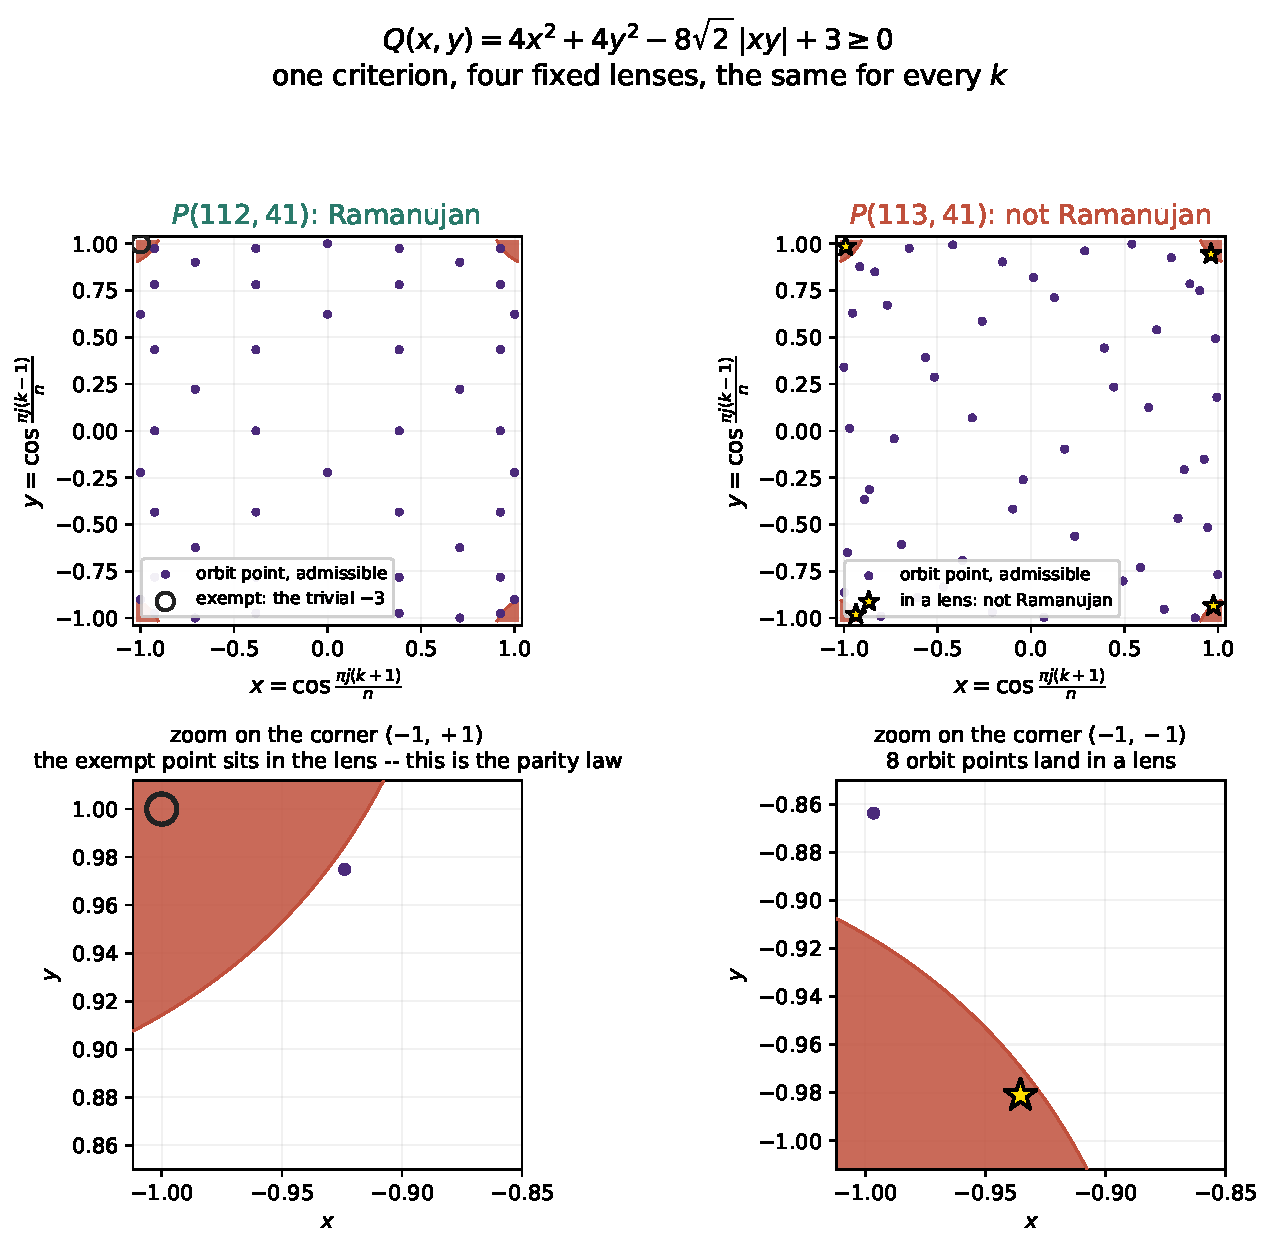
\includegraphics[width=\textwidth]{figures/fig_corner}
\caption{The corner criterion. Left, the largest Ramanujan member of the whole
family; right, the cover one step larger, which fails. The four forbidden
regions are the same in both pictures and for every $k$ --- only the map into
the square changes. In the left-hand zoom the single point inside a region is
the exempt trivial $-3$, which is why bipartiteness helps.}
\label{fig:corner}
\end{figure}

\section{Only finitely many, and a parity law}\label{sec:finite}

Both of the following come from the same observation: $D_k$ is negative at the
two points $u=\pm1$ where the grid $\{\cos(2\pi j/n)\}$ accumulates, so the grid
must \emph{clear} a band, and a fine grid cannot.

\begin{lemma}\label{lem:signs}
For every $k\ge1$,
\[
  D_k(1)=-7,\qquad D_k(0)\ge17,\qquad
  D_k(-1)=\begin{cases}-7,&k\text{ odd},\\ \ \ 9,&k\text{ even}.\end{cases}
\]
In particular $D_k$ has a root in $(0,1)$, and for odd $k$ also one in $(-1,0)$.
\end{lemma}

\begin{proof}
$T_k(1)=1$ gives $D_k(1)=11^2-8\cdot4^2=121-128=-7$. $T_k(-1)=(-1)^k$ gives
$D_k(-1)=(7-4(-1)^k)^2-8(2(-1)^k-2)^2$, which is $(-7)$ for $k$ odd and
$3^2-0=9$ for $k$ even. Finally $T_k(0)\in\{0,\pm1\}$, so
$D_k(0)=49-32\,T_k(0)^2\in\{49,17\}$. The sign changes give the roots.
\end{proof}

\begin{theorem}[Uniform finiteness, for every $k$]\label{thm:uniform}
Let $\tau=3-2\sqrt2=(\sqrt2-1)^2$. If $P(n,k)$ satisfies the Riemann Hypothesis
then
\[
  n\ \le\ \pi\bigl(2+\sqrt2\bigr)\sqrt{k^2+1},
\]
and if in addition $k$ and $n$ are both odd,
$n\le\tfrac12\pi(2+\sqrt2)\sqrt{k^2+1}$.
\end{theorem}

\begin{proof}
Write $x=\cos t$, $y=\cos kt$, and $a=1-x$, $b=1-y$, $s=a+b$. Suppose
$s<\tau$; then $a,b<\tau<1$, so $x,y>0$ and in particular $x+y>0$. Hence
$|A|=2(x+y)$ and $P=4xy$, and
\[
  G_k(t)=4\sqrt2\,(x+y)-4xy
        =\bigl(8\sqrt2-4\bigr)-\bigl(4\sqrt2-4\bigr)s-4ab .
\]
By AM--GM, $4ab\le s^2$, so $G_k(t)>7$ is implied by
\[
  s^2+\bigl(4\sqrt2-4\bigr)s\ <\ 8\sqrt2-11 .
\]
The left-hand side is increasing for $s\ge0$, and at $s=\tau$ it equals
\[
  (17-12\sqrt2)+(20\sqrt2-28)=8\sqrt2-11
\]
exactly. So $s<\tau$ suffices.

Now $1-\cos\theta\le\theta^2/2$ for every real $\theta$, whence
$s\le\bigl(1+k^2\bigr)t^2/2$, and therefore
\[
  0<t<\frac{\sqrt{2\tau}}{\sqrt{k^2+1}}=\frac{2-\sqrt2}{\sqrt{k^2+1}}
  \qquad\Longrightarrow\qquad G_k(t)>7,
\]
using $\sqrt{2\tau}=\sqrt{2}\,(\sqrt2-1)=2-\sqrt2$. The grid's smallest nonzero
angle is $2\pi/n$, so a Ramanujan $n$ needs
$2\pi/n\ge(2-\sqrt2)/\sqrt{k^2+1}$, i.e.\ $n\le2\pi\sqrt{k^2+1}/(2-\sqrt2)
=\pi(2+\sqrt2)\sqrt{k^2+1}$.

For the second bound take $k$ odd and put $t=\pi-\varphi$. Then $x=-\cos\varphi$
and, since $k$ is odd, $y=\cos(k\pi-k\varphi)=-\cos k\varphi$. With
$a'=1+x=1-\cos\varphi$ and $b'=1+y=1-\cos k\varphi$ and $s'=a'+b'<\tau$ we get
$x,y<0$, so $|A|=2(2-s')$ and $P=4(-1+a')(-1+b')$, and expanding gives
\emph{the same expression}
$\bigl(8\sqrt2-4\bigr)-\bigl(4\sqrt2-4\bigr)s'-4a'b'$. The rest of the argument
is verbatim, and $s'\le(1+k^2)\varphi^2/2$ as before. For odd $n$ the grid's
nearest point to $\pi$ is at $\varphi=\pi/n$, which gives the stated bound with
$\pi/n$ in place of $2\pi/n$ --- exactly half.
\end{proof}

\begin{remark}
An earlier draft of this work stated the same constant $\pi(2+\sqrt2)$, obtained
by expanding $\lambda_+$ to second order in $t$ at fixed $k$. That derivation is
\emph{invalid}: the critical $t$ scales like $1/k$, so $kt$ is of order one and
the expansion was used outside its domain. The constant survived numerical
testing only because the bound is loose. The proof above uses no expansion in
$kt$ at all --- only monotonicity, AM--GM, and $1-\cos\theta\le\theta^2/2$ ---
and holds for every $k$. The constant was right; the argument was not.
\end{remark}

\begin{theorem}[Finiteness]\label{thm:finite}
Let $u_k$ be the largest root of $D_k$ in $(-1,1)$. If $P(n,k)$ satisfies the
Riemann Hypothesis then
\[
  n\ \le\ \frac{2\pi}{\arccos u_k}\ =:\ B_k .
\]
In particular, for each $k$ only finitely many $n$ qualify.
\end{theorem}

\begin{proof}
By Lemma~\ref{lem:signs}, $D_k(1)=-7<0$, and $u_k$ is the largest root below
$1$, so $D_k<0$ throughout $(u_k,1]$. Suppose $n>B_k$. Then
$t=2\pi/n<\arccos u_k$, so $\cos t>u_k$ and hence $D_k(\cos t)<0$. The index
$j=1$ is never one of the two excluded indices of Corollary~\ref{cor:crit}
(that would need $n=2$), so Corollary~\ref{cor:crit} fails at $j=1$.
\end{proof}

Theorem~\ref{thm:uniform} is uniform but not sharp; for a \emph{given} $k$ the
exact root of $D_k$ does better, and that is what the classification uses.

Theorem~\ref{thm:uniform} bounds $n$ for each $k$, but the bound grows with
$k$, so it leaves open whether the family contains Ramanujan members of
arbitrarily large $k$. It does not, and the reason is that the failure
condition behind Theorem~\ref{thm:uniform} is a \emph{simultaneous Diophantine}
one, which Dirichlet's theorem satisfies unconditionally.

\begin{theorem}[Absolute finiteness]\label{thm:absolute}
If $n\ge231$ then $P(n,k)$ fails the Riemann Hypothesis for \emph{every} $k$.
Hence only finitely many generalized Petersen graphs satisfy it, and all of
them have $n\le230$.
\end{theorem}

\begin{proof}
The proof of Theorem~\ref{thm:uniform} shows that if
\[
  s=\bigl(1-\cos\tfrac{2\pi j}{n}\bigr)+\bigl(1-\cos\tfrac{2\pi jk}{n}\bigr)<\tau=3-2\sqrt2
\]
for even one nontrivial index $j$, then $P(n,k)$ is not Ramanujan. Writing
$\|\theta\|$ for the distance from $\theta$ to the nearest integer,
$1-\cos2\pi\theta=2\sin^{2}\pi\theta\le2\pi^{2}\|\theta\|^{2}$, so it is enough
that
\[
  \Bigl\|\tfrac jn\Bigr\|^{2}+\Bigl\|\tfrac{jk}{n}\Bigr\|^{2}
  \;<\;\frac{\tau}{2\pi^{2}}=0.0086919\ldots
\]
Let $J=\lfloor\sqrt n\rfloor$. Dirichlet's approximation theorem, applied to
the real number $k/n$, provides an integer $j$ with $1\le j\le J$ and
$\|jk/n\|\le1/(J+1)$. For that $j$ we have $J\le\sqrt n<J+1$, hence
\[
  \Bigl\|\tfrac jn\Bigr\|^{2}\le\Bigl(\tfrac Jn\Bigr)^{2}\le\frac1n,
  \qquad
  \Bigl\|\tfrac{jk}{n}\Bigr\|^{2}\le\frac{1}{(J+1)^{2}}<\frac1n ,
\]
so the left-hand side is less than $2/n$. Therefore $2/n<\tau/(2\pi^{2})$
suffices, that is
\[
  n\;>\;\frac{4\pi^{2}}{\tau}=230.097\ldots
\]
The index is legitimate: $1\le j\le\sqrt n<n/2$ once $n\ge5$, so $j$ is neither
$0$ nor the index $n/2$ that Corollary~\ref{cor:crit} excludes.
\end{proof}

\begin{remark}
The threshold $231$ is not sharp --- no Ramanujan $P(n,k)$ has $n$ above
$\RamAllMaxN$ --- and it does not need to be. Its only job is to be uniform in
$k$, which is exactly what the per-$k$ bound of Theorem~\ref{thm:finite} is
not. With it the classification becomes a finite problem in \emph{both}
variables: since $1\le k<n/2$, everything lives in $3\le n\le230$, a region
that can simply be exhausted.
\end{remark}

\begin{theorem}[Parity law]\label{thm:parity}
Let $k$ be odd and let $v_k$ be the smallest root of $D_k$ in $(-1,1)$. If $n$
is odd and $P(n,k)$ satisfies the Riemann Hypothesis then
\[
  n\ \le\ \frac{\pi}{\arccos(-v_k)} .
\]
No such restriction holds for even $n$, nor for even $k$.
\end{theorem}

\begin{proof}
For $k$ odd, $D_k(-1)=-7<0$ by Lemma~\ref{lem:signs}, so $D_k<0$ on
$[-1,v_k)$. The grid points nearest $t=\pi$ are $t=\pi(n\pm1)/n$ when $n$ is
odd, at distance $\pi/n$, with $\cos t=-\cos(\pi/n)$; and neither index is
excluded, since the excluded index $2j=n$ needs $n$ even. So the criterion
demands $-\cos(\pi/n)\ge v_k$, i.e.\ $\pi/n\ge\arccos(-v_k)$.

When $n$ is even the grid contains $t=\pi$ exactly, at $j=n/2$ -- and that is
precisely the index Corollary~\ref{cor:crit} excludes, because the sample there
is the trivial eigenvalue $-3$ of the bipartite graph. The band at $u=-1$ is
therefore invisible to even $n$. For even $k$, $D_k(-1)=9>0$ and there is no
band at $u=-1$ at all.
\end{proof}

The parity law is the reason the classification looks the way it does: for odd
$k$ the odd values of $n$ stop at roughly half the bound, and the tail of the
classification is even. It is also a small structural surprise -- \emph{being
bipartite helps}. Bipartiteness exempts the eigenvalue $-3$ from the Ramanujan
condition, and for odd $k$ that exemption is exactly what lets $n$ run twice as
far.

\section{The classification, certified exactly}\label{sec:ramcert}

Theorems~\ref{thm:finite} and~\ref{thm:parity} leave a finite computation, but a
finite computation is not yet a proof: the decision at a band edge is a
comparison of algebraic numbers, and that is where floating point fails
silently. We certify every case in exact arithmetic.

The mechanism is the one Corollary~\ref{cor:crit} makes available. Writing
$c_m=2\cos(2\pi jm/n)$ we have, by $4\cos a\cos b=2\cos(a+b)+2\cos(a-b)$,
\[
  A=c_1+c_k,\qquad P=c_{k+1}+c_{k-1},
\]
so $A$, $P$ and hence $D$ are values at $z=\zeta_n^{\,j}$ of Laurent
polynomials with integer coefficients. Since $\zeta_n^{\,j}$ is a primitive
$m$-th root of unity for $m=n/\gcd(n,j)$, each value is an algebraic integer of
$\mathbb Z[\zeta_m]$, and reducing modulo the cyclotomic polynomial $\Phi_m$
puts it in an exact integer coordinate vector. That vector vanishes if and only
if the value is exactly zero -- so the band-edge cases are decided by integer
arithmetic, with no estimate anywhere.

For the sign of a nonzero value we use the separation bound available to any
nonzero algebraic integer: the product of its conjugates is a nonzero rational
integer, so $|D|\ge1\big/\prod_{\sigma\ne1}|\sigma(D)|\ge 249^{-(\deg-1)}$,
using $|D|\le(7+4)^2+8\cdot4^2=249$ on the whole conjugate set. We evaluate at
a precision set from that bound and \emph{refuse} to report a sign unless the
computed value clears the guard, so a wrong sign is excluded rather than
improbable.

\begin{theorem}[Classification, per $k$]\label{thm:ramclass}
For every $k$ and every $n$, whether $P(n,k)$ satisfies the Riemann Hypothesis
is decided by Table~\ref{tab:ram}: for each $k$ listed there, the $n$ shown are
exactly those that qualify, and no $n>B_k$ qualifies, by
Theorem~\ref{thm:finite}. In particular there are exactly $\RamTotal$ such
graphs with $k\le\RamKmax$, from $\RamCases$ cases below the bound each decided
in exact arithmetic. That no $k$ beyond the table admits any $n$ at all is
Theorem~\ref{thm:absolute}, and the total is Theorem~\ref{thm:allk}.
\end{theorem}

\begin{table}[h]
\centering
\footnotesize
\setlength{\tabcolsep}{4pt}
% GENERATED by verification/verify_all.py -- do not edit by hand.
\begin{tabular}{r r r l}
\hline
$k$ & $B_k$ & count & the $n$ for which $P(n,k)$ satisfies the RH\\
\hline
$1$ & $15$ & $9$ & $3\text{--}8, 10, 12, 14$\\
$2$ & $23$ & $19$ & $5\text{--}23$\\
$3$ & $32$ & $18$ & $7\text{--}16, 18, 20, 22, 24, 26, 28, 30, 32$\\
$4$ & $42$ & $34$ & $9\text{--}42$\\
$5$ & $51$ & $28$ & $11\text{--}26, 28, 30, 32, 34, 36, 38, 40, 42, 44, 46, 48, 50$\\
$6$ & $61$ & $20$ & $13\text{--}16, 18, 20\text{--}23, 25, 27\text{--}28, 30, 32, 35, 37, 39, 42, 44, 49$\\
$7$ & $71$ & $39$ & $15\text{--}36, 38, 40, 42, 44, 46, 48, 50, 52, 54, 56, 58, 60, 62, 64, 66, 68, 70$\\
$8$ & $81$ & $16$ & $17, 19\text{--}22, 24, 26, 28\text{--}29, 31, 33, 35, 38, 40, 42, 49$\\
$9$ & $91$ & $50$ & $19\text{--}46, 48, 50, 52, 54, 56, 58, 60, 62, 64, 66, 68, 70, 72, 74, 76, 78, 80, 82, 84, 86, 88, 90$\\
$10$ & $101$ & $14$ & $21, 23, 25\text{--}26, 28, 30, 32, 34, 37, 39, 41, 43, 50, 52$\\
$11$ & $111$ & $36$ & $23\text{--}26, 28\text{--}32, 35\text{--}38, 40\text{--}42, 46\text{--}48, 50, 52\text{--}53, 58, 60, 62, 64, 70, 72, 74, 82, 84, 92, 94, 96, 104, 106$\\
$12$ & $121$ & $9$ & $27, 29\text{--}30, 32, 34, 38, 40, 45, 51$\\
$13$ & $131$ & $23$ & $28\text{--}30, 32, 34\text{--}37, 42\text{--}44, 46, 48\text{--}49, 56, 58, 60, 70, 72, 74, 84, 86, 98$\\
$14$ & $141$ & $7$ & $31, 33, 35\text{--}36, 38, 46, 53$\\
$15$ & $151$ & $19$ & $33\text{--}36, 38, 40\text{--}42, 49\text{--}50, 52, 54, 56, 66, 68, 70, 82, 84, 98$\\
$16$ & $161$ & $6$ & $35, 39\text{--}40, 42, 44, 52$\\
$17$ & $171$ & $16$ & $37\text{--}40, 42, 44, 46\text{--}47, 56, 58, 60, 62, 74, 76, 78, 94$\\
$18$ & $181$ & $3$ & $45\text{--}46, 50$\\
$19$ & $191$ & $17$ & $42\text{--}44, 46, 48, 50, 52\text{--}53, 64, 66, 68, 70, 84, 86, 88, 104, 106$\\
$20$ & $201$ & $3$ & $45, 49\text{--}50$\\
$21$ & $211$ & $11$ & $46, 48, 50, 54, 56, 58, 70, 72, 76, 92, 96$\\
$22$ & $221$ & $1$ & $49$\\
$23$ & $231$ & $10$ & $52\text{--}54, 56, 60, 62, 76, 78, 84, 106$\\
$24$ & $241$ & $1$ & $53$\\
$25$ & $251$ & $8$ & $56, 58, 60, 66, 68, 84, 90, 92$\\
$27$ & $271$ & $8$ & $60, 62, 64, 70, 72, 74, 90, 98$\\
$29$ & $291$ & $9$ & $64, 66, 68, 70, 76, 78, 96, 98, 106$\\
$31$ & $311$ & $4$ & $70, 74, 82, 84$\\
$33$ & $331$ & $5$ & $74, 76, 78, 86, 90$\\
$35$ & $351$ & $5$ & $78, 80, 84, 92, 96$\\
$37$ & $371$ & $3$ & $82, 84, 88$\\
$39$ & $391$ & $3$ & $88, 102, 106$\\
$41$ & $412$ & $2$ & $98, 112$\\
$43$ & $432$ & $2$ & $96, 98$\\
$45$ & $452$ & $2$ & $100, 108$\\
\hline
\multicolumn{4}{l}{\footnotesize No $k$ outside this table admits any $n$: the list is finite in both variables.}\\
\end{tabular}

\caption{The complete classification, every $n$ and every $k$. For each $k$,
$B_k$ is the per-$k$ bound of Theorem~\ref{thm:finite}; the rows stop at
$k=\RamAllMaxK$ because by Theorem~\ref{thm:absolute} no larger $k$ admits any
$n$ at all. Generated directly from the certification run.}
\label{tab:ram}
\end{table}

The bound is not merely finite but frequently sharp: at $k=2,3,4$ the largest
Ramanujan $n$ equals $\lfloor B_k\rfloor$ exactly, so the band at $u=1$ is the
only obstruction there, and the parity bound of Theorem~\ref{thm:parity} is
attained at $k=1,5,7,9$.

A floating-point classifier was run alongside the exact one throughout, as a
control with no authority: a disagreement is recorded as a failure of the run
rather than resolved in favour of either. It earned its place. At $k=1$ the
exponents of the Laurent polynomials collide ($k=1$ and $k-1=-(k-1)=0$), and an
implementation that built them as a dictionary literal silently discarded the
duplicated terms; the exact classifier then declared every $P(n,1)$ Ramanujan,
including $P(9,1)$, whose spectrum contains $2\cos(8\pi/9)-1=-2.879$. The
control caught all four affected values.

\begin{remark}
The classification is genuinely irregular in $k$. The largest Ramanujan $n$ is
not monotone --- $k=9$ reaches $n=\RamLastNine$ while $k=8$ and $k=10$ stop at
$\RamLastEight$ and $\RamLastTen$ --- because for even $k$ a third band, interior
to $(0,\pi)$ rather than at an endpoint, binds well before the band at $u=1$.
Locating those interior bands for general $k$ is exactly the question of which
cyclotomic reals avoid a semialgebraic set, and is where the Galois-orbit
machinery of Part~\ref{part:zf} applies.
\end{remark}

\section{The classification for every \texorpdfstring{$k$}{k}}\label{sec:allk}

Theorem~\ref{thm:absolute} confines the whole family to $3\le n\le230$, and
with $1\le k<n/2$ that region is finite. Exhausting it settles the question
completely.

\begin{theorem}[Complete classification]\label{thm:allk}
There are exactly $\RamAllTotal$ pairs $(n,k)$ with $n\ge3$ and $1\le k<n/2$
for which $P(n,k)$ satisfies the Riemann Hypothesis. They fall into
$\RamAllIso$ isomorphism classes. The largest is $n=\RamAllMaxN$, attained at
$k=41$; the largest $k$ that occurs at all is $\RamAllMaxK$; and the values of
$k$ that occur are $1,\dots,25$ together with the odd numbers from $27$ to
$\RamAllMaxK$. Every one of the $\RamAllCases$ cases in the region was decided
in exact arithmetic.
\end{theorem}

Two features of the answer are worth isolating. The first is that the list is
finite in \emph{both} variables, which Theorem~\ref{thm:uniform} alone does not
give: for each $k$ it allows $n$ up to $\pi(2+\sqrt2)\sqrt{k^{2}+1}$, a bound
that grows without limit, and only the Diophantine argument rules out large
$k$. The second is the parity asymmetry at the top of the range. Above $k=25$
no even $k$ occurs at all, while odd $k$ persists as far as $\RamAllMaxK$; this
is the parity law of Theorem~\ref{thm:parity} still operating at the end of the
list, where the exemption of the trivial $-3$ is the only thing keeping a
member alive.

\begin{remark}[Counting graphs rather than parameters]
$\RamAllTotal$ counts parameter pairs. $P(n,k)\cong P(n,\ell)$ exactly when
$\ell\equiv\pm k^{\pm1}\pmod n$, and quotienting by that relation leaves
$\RamAllIso$ graphs up to isomorphism. We report both because the first is
what the criterion decides and the second is what the classification is
\emph{about}; conflating them would overstate the count by a third.
\end{remark}

\section{Towards a closed form}\label{sec:closed}

Theorem~\ref{thm:allk} is a certified list, not a formula, and it is worth
being precise about what a formula would have to be. This section gives the
structure the list has; it stops short of a closed form, and \S\ref{sec:closed}
ends by saying exactly where.

The first observation is that the criterion is \emph{local at the divisors of
$n$}. Call $m$ the \emph{level} of the index $j$ if $m=n/\gcd(n,j)$; then
$\cos\frac{2\pi j}{n}$ is a primitive $m$-th value, and as $j$ ranges over all
indices of level $m$ the point ranges over the full conjugate set
$\{\cos\frac{2\pi i}{m}:\gcd(i,m)=1\}$. Say $m$ is \emph{bad for $k$} if some
primitive level-$m$ point violates $Q\ge0$.

\begin{theorem}[Locality]\label{thm:local}
$P(n,k)$ satisfies the Riemann Hypothesis if and only if no divisor $m\ge3$ of
$n$ is bad for $k$. Moreover badness at level $m$ depends on $k$ only through
$k\bmod m$.
\end{theorem}

\begin{proof}
Every index $j\in\{1,\dots,n-1\}$ has a level $m\mid n$, and $m\ge3$ unless
$j=0$ or $2j=n$ --- the two indices Corollary~\ref{cor:crit} excludes. Level
$m=2$ never obstructs in any case: there $u=-1$, and $D_k(-1)=9>0$ for even $k$
by Lemma~\ref{lem:signs}, while for odd $k$ the cover is bipartite and the point
carries the exempt trivial $-3$. So the criterion holds at every index exactly
when it holds at every primitive point of every level $m\ge3$ dividing $n$. The
last claim holds because the point
$\bigl(\cos\frac{\pi j(k+1)}{m},\cos\frac{\pi j(k-1)}{m}\bigr)$ is unchanged
when $k$ is replaced by $k+m$.
\end{proof}

\begin{corollary}[Divisor closure]\label{cor:divclosed}
If $P(n,k)$ satisfies the Riemann Hypothesis and $d\mid n$ with $d>2k$, then
$P(d,k)$ does too. For each $k$ the set of Ramanujan $n$ is closed downwards
under division, so it is determined by its minimal bad divisors --- and by
Theorem~\ref{thm:finite} only those below $B_k$ can matter.
\end{corollary}

\begin{proof}
The divisors of $d$ are divisors of $n$, so if none of the latter is bad for $k$
then none of the former is; apply Theorem~\ref{thm:local} twice.
\end{proof}

That reduces the classification to knowing which $(m,k\bmod m)$ are bad. The
next lemma is what converts that into arithmetic, and it is where the $\gcd$
enters.

\begin{lemma}[The minimum is a gcd]\label{lem:mingcd}
Let $\|\cdot\|$ denote distance to the nearest integer. If $m\nmid c$ then
\[
  \min\Bigl\{\,\Bigl\|\tfrac{jc}{m}\Bigr\|\ :\ \gcd(j,m)=1\,\Bigr\}
  \ =\ \frac{\gcd(c,m)}{m}.
\]
If $m\mid c$ the minimum is $0$.
\end{lemma}

\begin{proof}
Write $g=\gcd(c,m)$, $c=ga$, $m=gb$ with $\gcd(a,b)=1$, and $b>1$ since
$m\nmid c$. Then $jc\equiv g\,(ja)\pmod m$, so $\|jc/m\|=\|ja/b\|$ scaled: the
attainable residues are $g\,t$ with $t\equiv ja\pmod b$. As $j$ runs over the
units mod $m$, $j\bmod b$ runs over the units mod $b$, and $a$ is a unit there,
so $ja\bmod b$ runs over every unit of $b$ --- in particular over $1$. The
smallest nonzero residue attainable is therefore $g$, giving $g/m$, and $0$ is
not attainable because $b\nmid ja$ for $j$ a unit.
\end{proof}

Now the geometry pays. Corollary~\ref{cor:lens} showed the forbidden region
meets the sides of the square at distance $\tfrac32-\sqrt2$ from each corner, so
$Q<0$ forces \emph{both} $|x|$ and $|y|$ to be at least $\sqrt2-\tfrac12$. Since
$|\cos\pi t|\ge\sqrt2-\tfrac12$ exactly when $\|t\|\le\gamma$ for
\[
  \gamma=\frac{\arccos\bigl(\sqrt2-\tfrac12\bigr)}{\pi}=0.1328095\ldots,
  \qquad \frac1\gamma=7.5295\ldots,
\]
a level is safe as soon as one coordinate cannot come close enough --- and by
Lemma~\ref{lem:mingcd} that is a divisibility condition. Because $m/\gcd(k\pm1,m)$
is an integer and $1/\gamma$ is just above $7$, it is a condition on small
integers.

\begin{theorem}[Gcd safety]\label{thm:gcdsafe}
If $m/\gcd(k+1,m)\in\{2,\dots,7\}$ or $m/\gcd(k-1,m)\in\{2,\dots,7\}$, then $m$
is not bad for $k$.
\end{theorem}

\begin{proof}
Suppose $m/\gcd(k+1,m)=b$ with $2\le b\le7$. Then $m\nmid k+1$, so
Lemma~\ref{lem:mingcd} gives $\|j(k+1)/m\|\ge\gcd(k+1,m)/m=1/b\ge1/7>\gamma$ for
every $j$ coprime to $m$. Hence $|x|=|\cos\frac{\pi j(k+1)}{m}|<\sqrt2-\tfrac12$
at every primitive level-$m$ point, and $Q\ge0$ there by
Corollary~\ref{cor:lens}. The other case is identical.
\end{proof}

The value $b=1$ is excluded for a reason: $m\mid k+1$ pins $|x|=1$, which is the
worst case rather than the best, and Lemma~\ref{lem:mingcd} gives minimum $0$.

Theorem~\ref{thm:local} already gives the classification a pure form for
\emph{every} $k$: $P(n,k)$ is Ramanujan iff no divisor $m\ge3$ of $n$ is bad
for $k\bmod m$, and badness of a level is witnessed by a single index $j$ with
$Q<0$, an exact one-line check. Since $m\le\RamDirichlet$ by
Theorem~\ref{thm:absolute}, the whole classification is one theorem plus a
finite table of minimal bad levels (a few thousand pairs $(m,k\bmod m)$,
generated and stored with the verification record); the list of
$\RamAllTotal$ pairs is a consequence of that table, not the primary object.
For small $k$ the two bounds already in hand turn out to be the whole answer,
and this can be \emph{proved}, not merely checked: everything depends on where
$D_k$ is negative, and that is a question about the real roots of one integer
polynomial, which Sturm's theorem decides in integer arithmetic.

\begin{lemma}[Band structure]\label{lem:bands}
Let $u_k$ be the largest root of $D_k$ in $(-1,1)$. For
$k\in\{1,2,3,4,5,7,9\}$ the set where $D_k<0$ on $[-1,1]$ is exactly
\[
  (u_k,1]\quad(k\ \text{even}),\qquad\qquad [-1,-u_k)\cup(u_k,1]\quad(k\ \text{odd}).
\]
For $k=6,8$ and for every $k$ with $10\le k\le45$, $D_k$ has a further root in
$(-1,1)$ and is negative on an interval in the interior.
\end{lemma}

\begin{proof}
For odd $k$ the Chebyshev polynomial $T_k$ is odd, so $uT_k(u)$ is even and
$(2u+2T_k(u))^2$ is even; hence $D_k(-u)=D_k(u)$ and the roots come in pairs
$\pm u$, with $v_k=-u_k$ in the notation of Theorem~\ref{thm:parity}. For even
$k$, $D_k(-1)=9>0$ by Lemma~\ref{lem:signs}, so there is no band at $-1$. The
number of real roots of $D_k$ in $[-1,1]$, and the sign of $D_k$ between
consecutive roots, are decided by Sturm's theorem, a finite computation in
integer arithmetic on the coefficients of $D_k\in\mathbb Z[u]$; carried out
exactly for $k\le45$ (\texttt{verification/interior\_bands.py}, which isolates
the roots over $\mathbb Q$ and evaluates $D_k$ at rational points between them),
it finds one root in $(-1,1)$ for $k=2,4$, two for $k=1,3,5,7,9$, and at least
three for every other $k\le45$, with the signs stated. For $k=2$ the whole
computation fits on a page: $D_2(u)=64u^6-192u^4-16u^3+112u^2+8u+17$ has
$D_2(-1)=9$, $D_2(0.96)=0.765\ldots>0$ and $D_2(1)=-7$; Sturm's theorem gives
$D_2$ no root in $[-1,0.96]$, and $D_2'$ no root in $(0.96,1)$, so $D_2$ is
positive on $[-1,0.96]$ and crosses zero exactly once in $(0.96,1)$, at
$u_2=0.9641\ldots$.
\end{proof}

\begin{theorem}[Closed form for $k\le9$]\label{prop:closedsmall}
Let $B_k=2\pi/\arccos u_k$ be the bound of Theorem~\ref{thm:finite} and
$P_k=\pi/\arccos u_k=B_k/2$ that of Theorem~\ref{thm:parity}. Then
\[
\begin{array}{ll}
  k=2,4: & P(n,k)\ \text{is Ramanujan}\iff 2k<n\le B_k;\\[2pt]
  k=1,3,5,7,9: & P(n,k)\ \text{is Ramanujan}\iff 2k<n\le B_k\ \text{and }
  (n\ \text{even or}\ n\le P_k).
\end{array}
\]
Equivalently, for odd $k$: $2k<n\le B_k$ and every odd divisor of $n$ is at most
$P_k$.
\end{theorem}

\begin{proof}
By Theorem~\ref{thm:crit}, $P(n,k)$ is Ramanujan iff $D_k(\cos\frac{2\pi j}{n})\ge0$
for every $j$ with $1\le j\le n-1$ and $j\ne n/2$. By Lemma~\ref{lem:bands},
$D_k(\cos t)<0$ exactly when $\cos t>u_k$, or $k$ is odd and $\cos t<-u_k$.

\emph{The band at $1$.} Among $1\le j\le n-1$ the largest value of
$\cos\frac{2\pi j}{n}$ is $\cos\frac{2\pi}{n}$, at $j=1$ and $j=n-1$. So some
grid point lies in $(u_k,1]$ iff $\cos\frac{2\pi}{n}>u_k$ iff $n>B_k$.

\emph{The band at $-1$ (odd $k$).} Write $d=n-2j$, so that
$\cos\frac{2\pi j}{n}=-\cos\frac{\pi d}{n}$, and $d\ne0$ because $j=n/2$ is the
excluded trivial index. A grid point lies in $[-1,-u_k)$ iff
$\cos\frac{\pi d}{n}>u_k$ for some admissible $d$, and the admissible $|d|$ are
the positive integers of the same parity as $n$. The smallest is $2$ when $n$ is
even, giving the condition $\cos\frac{2\pi}{n}>u_k$ again, i.e.\ $n>B_k$; and
$1$ when $n$ is odd, giving $\cos\frac{\pi}{n}>u_k$, i.e.\ $n>P_k$.

The lower bound $2k<n$ is the standing hypothesis $k<n/2$. For the equivalent
form: an even $n\le B_k$ has every odd divisor at most $n/2\le P_k$, and an odd
$n$ is its own odd divisor.
\end{proof}

For even $k$ there is no band at $u=-1$ at all, which is why $k=2$ and $k=4$
are unbroken runs; for odd $k$ the second band contributes exactly the
constraint that $n$ carry no large odd divisor, which by
Corollary~\ref{cor:divclosed} is the natural form for a divisor-closed set to
take. The thresholds themselves --- $\lfloor B_k\rfloor$ and $\lfloor P_k\rfloor$
--- are $\lfloor B_k\rfloor=\RamLastTwo,\RamLastThree,\RamLastFour,\RamLastFive,\RamLastSeven,\RamLastNine$
at $k=2,3,4,5,7,9$ (Table~\ref{tab:ram}); deciding whether
$\cos\frac{2\pi}{n}\le u_k$ at the boundary $n$ is one exact comparison in
$\mathbb Z[\zeta_n]$, as in \S\ref{sec:ramcert}.

\begin{remark}[What a closed form still needs, and why we do not have one]
Three things are missing. Theorem~\ref{thm:gcdsafe} is \emph{sufficient and
one-sided}: it certifies safety and says nothing about badness, and a closed
form needs both directions. Theorem~\ref{prop:closedsmall} stops at
$k=6,8$ and at every $k\ge10$ --- precisely where Lemma~\ref{lem:bands} finds an
interior band, neither at $u=1$ nor at $u=-1$, and locating which grid points
fall into those bands is the question of which cyclotomic reals avoid a
semialgebraic set that \S\ref{sec:ramcert} already flagged. And nothing here explains the shape of the
answer at the top of the range: we can prove no $P(n,k)$ with
$k>\RamAllMaxK$ is Ramanujan, but only by exhausting the finitely many cases
Theorem~\ref{thm:absolute} leaves, and we cannot say why the cut falls at
$\RamAllMaxK$ rather than near it. The list is complete and certified; it is
not yet explained.
\end{remark}

\section{Every cubic cyclic cover}\label{sec:covram}

Nothing in \S\ref{sec:corner} used $P(n,k)$ beyond two facts: the base has two
vertices, and the cover is cubic. The criterion therefore belongs to the
setting of \S\ref{sec:covers} rather than to this family, and saying so turns
a classification of one family into a statement about a class of covers.

A cubic base on two vertices is one of exactly two things. A loop absorbs two
of the three half-edges at its vertex, so a vertex carries at most one loop,
and a vertex with a loop has exactly one non-loop edge. Either both vertices
carry loops --- the \emph{two-loop base} $B(a,b,c)$, with a loop of voltage $a$
at $u$, a loop of voltage $b$ at $v$, and an edge $u\!-\!v$ of voltage $c$ ---
or neither does, leaving three parallel edges, the \emph{theta base}
$T(c_1,c_2,c_3)$. We have $P(n,k)=B(1,k,0)^{n}$, and the covers of a theta base
are the cubic cyclic Haar graphs, which are bipartite.

\begin{theorem}[Corner criterion on a two-loop base]\label{thm:covcorner}
Let $X=B(a,b,c)^{n}$ be simple and connected. Then $X$ satisfies the Riemann
Hypothesis if and only if
\[
  Q\Bigl(\cos\tfrac{\pi j(a+b)}{n},\ \cos\tfrac{\pi j(a-b)}{n}\Bigr)\ \ge\ 0
\]
at every nontrivial index, with $Q$ the form of Theorem~\ref{thm:corner}.
In particular the spectrum, and hence the answer, does not depend on the edge
voltage $c$ at all.
\end{theorem}

\begin{proof}
By Theorem~\ref{thm:cover} the character block is
$M_j=\begin{psmallmatrix}\alpha_j&\omega^{jc}\\ \omega^{-jc}&\beta_j\end{psmallmatrix}$
with $\alpha_j=2\cos\frac{2\pi ja}{n}$ and $\beta_j=2\cos\frac{2\pi jb}{n}$.
Its characteristic polynomial is $\lambda^{2}-(\alpha+\beta)\lambda+(\alpha\beta-|\omega^{jc}|^{2})$,
and $|\omega^{jc}|=1$, so it is $\lambda^{2}-A\lambda+(P-1)$ exactly as in
Lemma~\ref{lem:blocks} --- with no $c$ in it. The derivation of
Theorem~\ref{thm:crit} used only $|\alpha|,|\beta|\le2$, so it applies verbatim,
and the substitution of Theorem~\ref{thm:corner} applies with $a+b$ and $a-b$
in place of $k+1$ and $k-1$, because
$\alpha+\beta=4\cos\frac{\pi j(a+b)}{n}\cos\frac{\pi j(a-b)}{n}$ and
$\alpha\beta=2\bigl(\cos\frac{2\pi j(a+b)}{n}+\cos\frac{2\pi j(a-b)}{n}\bigr)$.
\end{proof}

\begin{theorem}[Theta base]\label{thm:thetarh}
$T(c_1,c_2,c_3)^{n}$ satisfies the Riemann Hypothesis if and only if
\[
  \sum_{l<m}\cos\frac{2\pi j(c_l-c_m)}{n}\ \le\ \frac52
  \qquad\text{for every }j\ne0 .
\]
\end{theorem}

\begin{proof}
The block is $\begin{psmallmatrix}0&S_j\\ \overline{S_j}&0\end{psmallmatrix}$
with $S_j=\sum_l\omega^{jc_l}$, so its eigenvalues are $\pm|S_j|$ and the cover
is bipartite. Now $|S_j|^{2}=3+2\sum_{l<m}\cos\frac{2\pi j(c_l-c_m)}{n}$, and
the Ramanujan condition on a nontrivial index is $|S_j|^{2}\le8$.
\end{proof}

\begin{theorem}[Uniform finiteness on both bases]\label{thm:covfinite}
Writing voltages by their representatives of least absolute value, and $d_1,d_2,d_3$
for the pairwise differences $c_l-c_m$,
\begin{align*}
  B(a,b,c)^{n}\ \text{Ramanujan}\ &\Longrightarrow\ n\le\pi(2+\sqrt2)\sqrt{a^{2}+b^{2}},\\
  T(c_1,c_2,c_3)^{n}\ \text{Ramanujan}\ &\Longrightarrow\ n\le2\pi\sqrt{d_1^{2}+d_2^{2}+d_3^{2}} .
\end{align*}
\end{theorem}

\begin{proof}
The first is the proof of Theorem~\ref{thm:uniform} with $\cos\frac{2\pi ja}{n}$
and $\cos\frac{2\pi jb}{n}$ in place of $\cos t$ and $\cos kt$; the estimate
$1-\cos\theta\le\theta^{2}/2$ now gives $s\le(a^{2}+b^{2})\theta^{2}/2$, and
setting $\theta=2\pi/n$ gives the bound. Specialising to $(a,b)=(1,k)$ returns
Theorem~\ref{thm:uniform} exactly. For the second, the condition of
Theorem~\ref{thm:thetarh} fails as soon as $\sum_l(1-\cos\frac{2\pi jd_l}{n})<\tfrac12$,
and that sum is at most $\theta^{2}\sum_ld_l^{2}/2$; at $j=1$ this forces
failure once $2\pi/n<1/\sqrt{\sum d_l^{2}}$.
\end{proof}

The second bound is sometimes attained exactly: for $T(0,1,2)$ it reads
$n\le2\pi\sqrt6=15.39\ldots$, and $n=15$ is Ramanujan.

Both bases are therefore finite, and the reason is not special to two-vertex
bases.

\begin{theorem}[No infinite family is a cyclic cover]\label{thm:noinfinite}
Let $B$ be a fixed finite connected cubic base with integer voltages. Then
$B^{n}$ is Ramanujan for only finitely many $n$. Explicitly, writing $L$ for
$\sqrt2\sum|v_e|$ over the non-loop edges and $R$ for $\sum v_e^{2}$ over the
loops, $B^{n}$ is not Ramanujan as soon as
\[
  \frac{2\pi}{n}L+\Bigl(\frac{2\pi}{n}\Bigr)^{2}R\;<\;\tau=3-2\sqrt2 .
\]
\end{theorem}

\begin{proof}
$M_0$ is the adjacency matrix of the base, which is $3$-regular, so its largest
eigenvalue is $3$. A non-loop edge of voltage $v$ moves two entries of $M_1$ by
$|\omega^{v}-1|\le2\pi|v|/n$ each, and a loop of voltage $v$ moves one entry by
$|2\cos\frac{2\pi v}{n}-2|\le(2\pi v/n)^{2}$; summing gives
$\|M_1-M_0\|_2\le\|M_1-M_0\|_F\le\frac{2\pi}{n}L+(\frac{2\pi}{n})^{2}R$. By
Weyl's inequality $\lambda_{\max}(M_1)\ge3-\|M_1-M_0\|_2$, and $\lambda_{\max}(M_1)$
is a nontrivial eigenvalue, since in a connected cover the eigenvalue $3$ has
multiplicity one and occurs at $j=0$. So once the displayed quantity is below
$3-2\sqrt2$ the cover has a nontrivial eigenvalue exceeding $2\sqrt2$.
\end{proof}

\begin{remark}[What this is, and is not]
Theorem~\ref{thm:noinfinite} says that no construction of the kind this paper
studies can produce an infinite family of Ramanujan graphs --- the no-go is a
property of the class, not a limitation of our search. We claim no novelty for
the principle: it is the cyclic instance of the familiar fact that abelian
covers do not expand, which is precisely why the Lubotzky--Phillips--Sarnak
construction \cite{lps} is built on $\mathrm{PGL}_2$ and not on a cyclic group.
What is new here is the explicit constant, and the two exact criteria of
Theorems~\ref{thm:covcorner} and~\ref{thm:thetarh} for the two-vertex bases,
which decide the finitely many surviving cases rather than merely bounding
them.
\end{remark}

\section{The deficit: what the no-go costs}\label{sec:deficit}

A classification that ends in a finite list tells a designer that beyond a
certain size there is nothing optimal to build. That is not by itself useful
advice. The useful quantity is how much is lost, and the criterion supplies it
in closed form.

\begin{definition}
For a cover with nontrivial spectral radius $\lambda_2$, the \emph{deficit} is
$\delta=\lambda_2-2\sqrt2$, and for a given size,
$\delta^{*}(n)=\min_{1\le k<n/2}\delta(n,k)$.
\end{definition}

$\delta^{*}(n)\le0$ exactly when some $P(n,k)$ is Ramanujan, which by
Theorem~\ref{thm:allk} happens for exactly $\RamAllSizes$ values of $n$, the
largest being $\RamAllMaxN$.

\begin{proposition}\label{prop:deficit}
$\delta(n,k)<3-2\sqrt2$ for every $n$ and $k$, and
$\sup_{n,k}\delta(n,k)=3-2\sqrt2$, approached as $n\to\infty$.
\end{proposition}

\begin{proof}
$\lambda_2<3$ because $3$ is simple in a connected cubic graph, which gives the
bound. For the supremum, at $j=1$ the block $M_1$ tends to $M_0$ as
$n\to\infty$, so its top eigenvalue tends to $3$, and it is nontrivial.
\end{proof}

So the loss is bounded, and the bound is exactly the gap $\tau$ that the whole
argument has been about: an engineer who builds at a size where no optimal
member exists gives up at most $3-2\sqrt2=0.1716\ldots$ in nontrivial spectral
radius, and that is the worst case rather than a typical one.
Figure~\ref{fig:deficit} plots $\delta^{*}$. Its two branches are the parity
law once more: for one parity of $n$ the exemption of the trivial $-3$ is
available and for the other it is not.

\begin{figure}[h]
\centering
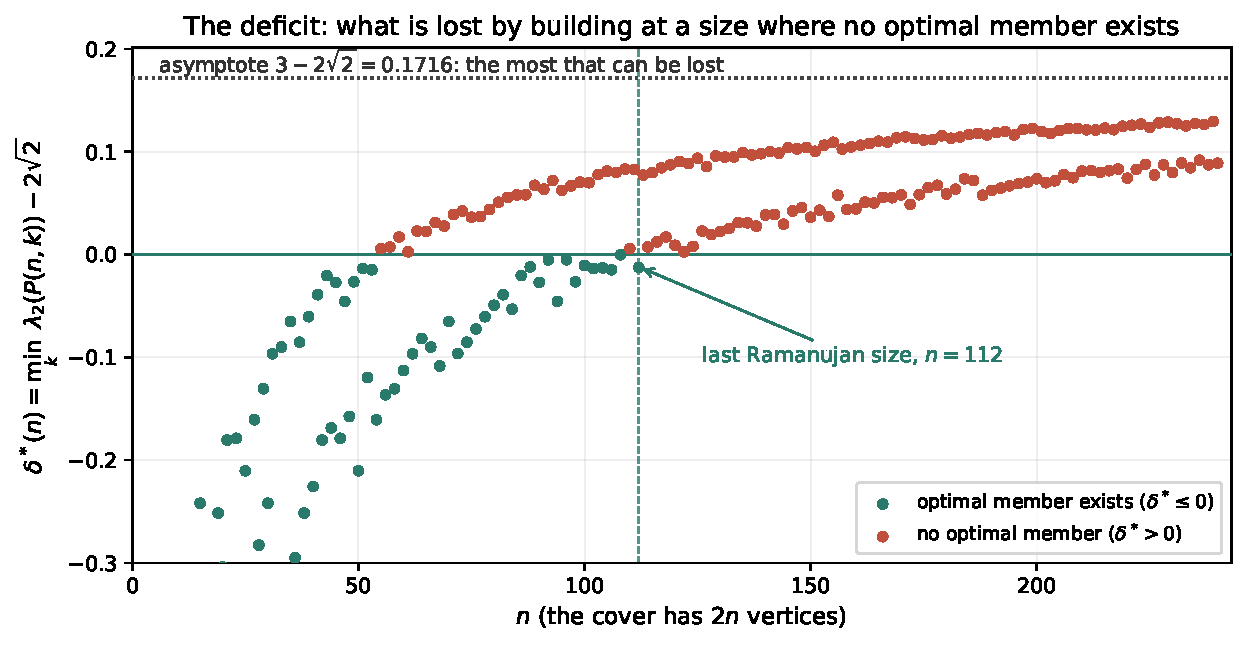
\includegraphics[width=\textwidth]{figures/fig_deficit}
\caption{The deficit $\delta^{*}(n)$, the best achievable nontrivial spectral
radius at each size, measured from the Ramanujan threshold. Green points are
sizes at which an optimal member exists; the last is $n=\RamAllMaxN$. The
curve rises to the asymptote $3-2\sqrt2$, which by
Proposition~\ref{prop:deficit} is the most that can ever be lost. The two
branches are the parity law.}
\label{fig:deficit}
\end{figure}


\part{Maximum Nullity and Zero Forcing on Cyclic Covers}
\label{part:zf}

\section{Background}
Given a set $S$ of \emph{filled} vertices of a graph $G$, the colour change
rule says: if a filled vertex has exactly one unfilled neighbour, that
neighbour becomes filled. Write $\mathrm{cl}(S)$ for the closure of $S$ under
repeated application. $S$ is a \emph{zero forcing set} if $\mathrm{cl}(S)=V$,
and $Z(G)$ is the least size of one. $Z(G)$ bounds the maximum nullity over
the symmetric matrices with $G$'s off-diagonal pattern, and arose
independently in the control of quantum systems and in sensor placement for
power networks.

The families we treat all have $2n$ or $4n$ vertices, are cubic, and carry the
rotation $\rho:i\mapsto i+1$ acting on index subscripts.

\begin{itemize}
\item $P(n,k)$: outer $u_iu_{i+1}$, inner $v_iv_{i+k}$, spokes $u_iv_i$.
\item $I(n,j,k)$: outer $u_iu_{i+j}$, inner $v_iv_{i+k}$, spokes $u_iv_i$;
      thus $P(n,k)=I(n,1,k)$.
\item $DP(n,k)$: two outer cycles $u_iu_{i+1}$ and $x_ix_{i+1}$, inner edges
      $w_iy_{i+k}$ and $y_iw_{i+k}$, spokes $u_iw_i$ and $x_iy_i$.
\end{itemize}

Rashidi, Shajareh Poursalavati and Tavakkoli \cite{RST} proved
$Z(P(n,k))\le2k+2$ and $Z(P(n,2))=6$ for $n\ge10$. Their Theorem 3.6, claiming
$Z(P(n,3))=8$ for $n\ge12$, is false: Krishnan \cite{K} exhibits
$Z(P(12,3))=7$, the flaw being a case analysis that never excludes $7$-vertex
sets. That note states as its Conjecture 5 that $Z(P(n,3))=8$ for every $n\ge13$,
identifying the missing ingredient as ``a lower-bound proof valid for all large
$n$'', and closes by recording that
\begin{quote}\itshape
``Determining $Z(P(n,k))$ for general $k$ --- the stabilization threshold and a
rigorous lower bound for $k\ge4$ --- remains open.''
\end{quote}
We settle all three. Theorem~\ref{thm:k3krishnan} proves Conjecture 5 and so
fixes the threshold at $13$; Theorems~\ref{thm:certvals} and \ref{thm:k3all}
give rigorous lower bounds, indeed exact values, for $k=4$, and determine the
whole $k=4$ sequence.

\section{The rotation bootstrap}
The following two lemmas are elementary; the point is that together they
reduce an ``all $n$'' statement to one finite check.

\begin{lemma}[Bootstrap]\label{lem:boot}
Let $\rho$ be an automorphism of a finite graph $G$ and let $S\subseteq V(G)$
satisfy $\rho(S)\subseteq \mathrm{cl}(S)$. Then
$\rho(\mathrm{cl}(S))=\mathrm{cl}(S)$.
\end{lemma}

\begin{proof}
Closure commutes with automorphisms, and is monotone and idempotent, so
$\rho(\mathrm{cl}(S))=\mathrm{cl}(\rho(S))\subseteq
\mathrm{cl}(\mathrm{cl}(S))=\mathrm{cl}(S)$. As $\rho$ permutes the finite set
$V(G)$, the two sets have equal cardinality, hence are equal.
\end{proof}

\begin{lemma}[Closing]\label{lem:close}
Let $G$ be cubic with vertex set $O\sqcup I$ such that every vertex of $I$ has
exactly one neighbour in $O$, every vertex of $O$ has exactly one neighbour in
$I$, and the remaining neighbours of each vertex of $O$ lie in $O$. If
$O\subseteq \mathrm{cl}(S)$ then $\mathrm{cl}(S)=V(G)$.
\end{lemma}

\begin{proof}
Suppose some $w\in I$ is unfilled and let $o\in O$ be its unique neighbour in
$O$. The other two neighbours of $o$ lie in $O$, hence are filled, so $w$ is
the unique unfilled neighbour of the filled vertex $o$ and is forced.
\end{proof}

To apply these to a family it suffices to exhibit one set $S$, described
uniformly in $n$, and verify $\rho(S)\subseteq\mathrm{cl}(S)$ by an explicit
finite forcing chain. Since $\rho$'s orbit of any outer vertex is all of $O$,
Lemmas~\ref{lem:boot} and \ref{lem:close} then give $\mathrm{cl}(S)=V$ and so
$Z(G)\le|S|$, for every $n$ in range.

\section{I-graphs}
\begin{theorem}\label{thm:I}
For all $j,k\ge1$ and $n\ge 2(j+k)+1$, $\;Z(I(n,j,k))\le 2(j+k)$.
\end{theorem}

\begin{proof}
Put $m=2(j+k)$ and $S=\{u_0,\dots,u_{m-1}\}$, so $|S|=m$. Since
$n\ge m+1$ the indices $0,\dots,m$ are pairwise distinct mod $n$.

\emph{Step 1.} The outer neighbours of $u_i$ are $u_{i\pm j}$, both in $S$
precisely when $j\le i\le m-1-j$. For such $i$ the spoke neighbour $v_i$ is
therefore the unique unfilled neighbour of $u_i$ and is forced. This fills
$v_j,\dots,v_{m-1-j}$, that is $v_j,\dots,v_{j+2k-1}$.

\emph{Step 2.} Consider $v_{j+k}$. Its neighbours are $u_{j+k}\in S$ (as
$j+k\le m-1$), $v_{j}$, filled in Step 1, and $v_{j+2k}$, which is not:
Step 1 filled indices at most $j+2k-1$. So $v_{j+k}$ forces $v_{j+2k}$.

\emph{Step 3.} Consider $u_{j+2k}=u_{m-j}$. Its neighbours are $u_{2k}\in S$
(as $2k\le m-1$, using $j\ge1$), the vertex $v_{j+2k}$ filled in Step 2, and
$u_{m}$, which is unfilled. So $u_{j+2k}$ forces $u_m$.

Hence $\rho(S)=\{u_1,\dots,u_m\}\subseteq\mathrm{cl}(S)$. By
Lemma~\ref{lem:boot}, $\mathrm{cl}(S)$ is $\rho$-invariant; it contains $u_0$,
whose $\rho$-orbit is all of $O=\{u_0,\dots,u_{n-1}\}$, so $O\subseteq
\mathrm{cl}(S)$, and Lemma~\ref{lem:close} gives $\mathrm{cl}(S)=V$.
\end{proof}

\begin{corollary}
For $k\ge1$ and $n\ge2k+3$, $Z(P(n,k))\le 2k+2$.
\end{corollary}

\begin{proof}
$P(n,k)=I(n,1,k)$; take $j=1$ in Theorem~\ref{thm:I}.
\end{proof}

\begin{remark}
The corollary is \cite[Thm.~2.2]{RST}. We note it because that paper is known
to contain a false theorem, and because the corrected argument given in
\cite{K} is written only for $k=3$; the proof above is uniform in $j$ and $k$.
Every step of the chain has been verified by computer for $1\le j\le4$,
$1\le k\le5$ and six values of $n$ per pair (106 cases).
\end{remark}

\begin{remark}[Scope]\label{rem:scope}
Theorem~\ref{thm:I} should not be read as $2(j+k)$ new bounds. If
$\gcd(n,j)=1$ then multiplying indices by $j^{-1}\bmod n$ is an isomorphism
$I(n,j,k)\cong I(n,1,j^{-1}k)=P(n,j^{-1}k)$, so those graphs are generalized
Petersen graphs and the corollary already applies. We verified this in five
cases, e.g.\ $I(15,2,4)\cong P(15,2)$ with $Z=6$ on both sides and
$I(13,2,5)\cong P(13,4)$ with $Z=8$. The genuinely new content of
Theorem~\ref{thm:I} is therefore confined to $\gcd(n,j)>1$ and $\gcd(n,k)>1$.

In that regime the bound is usually far from sharp: among the cases we
computed it is attained only at $I(18,2,3)$ ($Z=10=2(2+3)$), while e.g.\
$I(20,5,8)$ has $Z=10$ against a bound of $26$. The reason is structural. When
$\gcd(n,j)=d>1$ the outer vertices form $d$ cycles of length $n/d$ rather than
one cycle, and the set $\{u_0,\dots,u_{m-1}\}$ used in the proof spreads across
all of them; a smaller, better-adapted set suffices. We record the bound as
proved and its sharpness in this regime as open.
\end{remark}

\section{Double generalized Petersen graphs}
\begin{theorem}\label{thm:DP}
For all $k\ge1$ and $n\ge2k+3$, $\;Z(DP(n,k))\le 4k+4$.
\end{theorem}

\begin{proof}
Put $S=\{u_0,\dots,u_{2k+1}\}\cup\{x_0,\dots,x_{2k+1}\}$, so $|S|=4k+4$.

\emph{Step 1.} For $1\le i\le 2k$ the outer neighbours $u_{i\pm1}$ of $u_i$
lie in $S$, so $u_i$ forces $w_i$; symmetrically $x_i$ forces $y_i$. This
fills $w_1,\dots,w_{2k}$ and $y_1,\dots,y_{2k}$.

\emph{Step 2.} The neighbours of $w_{k+1}$ are $u_{k+1}\in S$, $y_1$ (filled)
and $y_{2k+1}$ (not), so $w_{k+1}$ forces $y_{2k+1}$. Symmetrically $y_{k+1}$
forces $w_{2k+1}$.

\emph{Step 3.} The neighbours of $u_{2k+1}$ are $u_{2k}\in S$, $w_{2k+1}$
(filled in Step 2) and $u_{2k+2}$, so $u_{2k+1}$ forces $u_{2k+2}$;
symmetrically $x_{2k+1}$ forces $x_{2k+2}$.

Hence $\rho(S)\subseteq\mathrm{cl}(S)$. The outer set here is
$O=\{u_i\}\cup\{x_i\}$, on which $\rho$ acts with two orbits, both met by
$\mathrm{cl}(S)$; Lemmas~\ref{lem:boot} and \ref{lem:close} finish as before.
\end{proof}

\noindent
No zero forcing results for $DP(n,k)$ were found in the literature; the family
is studied for Hamiltonicity, super-connectivity and its automorphism group.
Every step above was verified by computer for $1\le k\le5$ and eight values of
$n$ per $k$.

\section{Computed values}
All values are exact, by exhaustive search over vertex subsets with a
$128$-bit mask closure, reduced by $\rho$: a minimum forcing set may be assumed
to contain a fixed orbit representative. The implementation reproduced every
published value before use --- Krishnan's table of $Z(P(n,3))$ for
$7\le n\le20$ (including the corrected $Z(P(12,3))=7$ and the non-monotone
values at $n=10,11$), $Z(P(n,2))=6$ for $10\le n\le16$, and
$Z(P(2k+1,k))=6$ for $k=5,6,7$ --- and was independently cross-checked against
a brute-force implementation and two exact solver formulations.

\begin{figure}[h]\centering
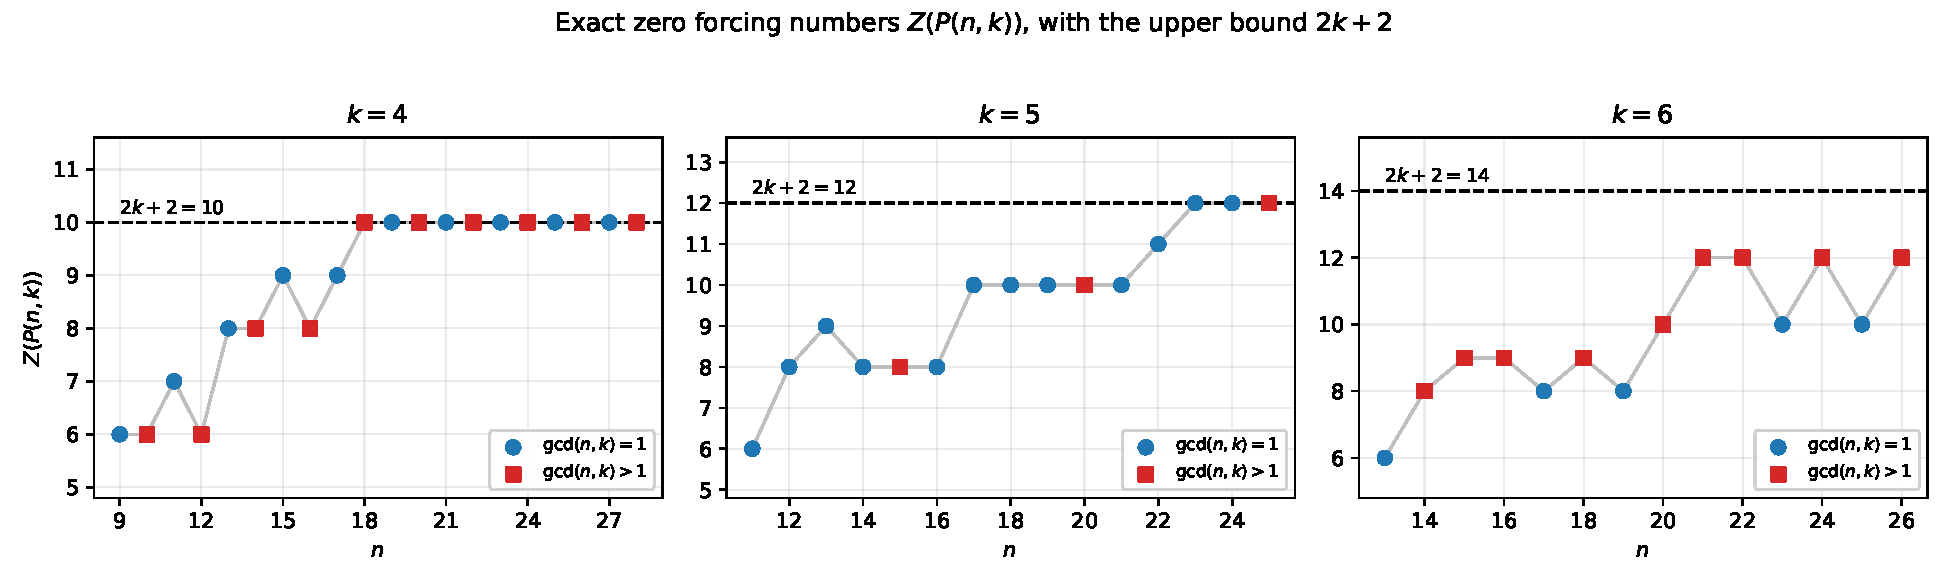
\includegraphics[width=\textwidth]{figures/zf_sequences.pdf}
\caption{Exact $Z(P(n,k))$ for $k=4,5,6$ against the bound $2k+2$. Points are
separated by whether $\gcd(n,k)=1$. The sequences are non-monotone: $k=4$
drops at $n=12,16$ and $k=6$ at $n=23,25$.}
\end{figure}

\begin{table}[h]\centering
\begin{tabular}{llll}
\toprule
$k$ & bound $2k+2$ & least $n$ attaining it & least $n$ from which it holds always \\
\midrule
2 & 6  & 7  & $9$ \ (it fails at $n=8$) \\
3 & 8  & 10 & $13$ \ (it fails at $n=11,12$) \\
4 & 10 & 18 & $18$ \ (Theorem~\ref{thm:complete}) \\
5 & 12 & 23 & not determined \\
6 & 14 & 28 & not determined; $Z(P(29,6))=12$ \\
\bottomrule
\end{tabular}
\caption{The bound is attained well before it is attained \emph{always}: at
$k=3$ it first holds at $n=10$, fails again at $n=11$ and $12$, and holds for
every $n\ge13$ (Theorem~\ref{thm:k3krishnan}). The two columns are different
quantities and conflating them is easy; at $k=6$ the bound is attained at
$n=28$ and lost at $n=29$, so no stabilization threshold is known there. At
$k=4$ the two columns happen to coincide at $18$, which is not a pattern: they
differ at $k=2$ and $k=3$.
All values by exhaustive search.}
\end{table}

\begin{conjecture}\label{conj}
For each fixed $k$ and each $d\mid k$, the values $Z(P(n,k))$ over $n$ with
$\gcd(n,k)=d$ are eventually constant and equal to $2k+2$.
\end{conjecture}

\noindent
An earlier form of this conjecture, asserting a single threshold
$n_0(k)=5k-2$ beyond which $Z(P(n,k))=2k+2$ for \emph{all} $n$, is false. It
fits $k=3,4,5$, and predicted that $n=28$ would be the first $n$ with
$Z(P(n,6))=14$; that prediction, recorded before the computation finished, was
borne out. But $Z(P(29,6))=12$, and $29>28$, so $28$ is not a stabilization
point and the single-threshold form fails at $k=6$.

The explanation is $\gcd(n,k)$. Sorting the $k=6$ data by $d=\gcd(n,6)$:

\begin{center}
\begin{tabular}{cll}
\toprule
$d$ & $n$ & $Z(P(n,6))$ \\
\midrule
1 & 13, 17, 19, 23, 25, 29 & 6, 8, 8, 10, 10, 12 \\
2 & 14, 16, 20, 22, 26, 28 & 8, 9, 10, 12, 12, 14 \\
3 & 15, 21, 27 & 9, 12, 13 \\
6 & 18, 24 & 9, 12 \\
\bottomrule
\end{tabular}
\end{center}

\noindent
Each class climbs on its own schedule: the class $d=2$ attains $14$ at $n=28$
while the coprime class has only reached $12$ by $n=29$. At $k=4$ and $k=5$ all
classes had converged within the computed range, which is why a single
threshold appeared to fit; at $k=6$ they separate. The thresholds $10,13,18,23$
for $k=2,3,4,5$ should therefore be read as the point at which the slowest
class happened to arrive, not as values of a formula.

For $DP$, our computed values give $Z(DP(n,1))=8=4\cdot1+4$ for $6\le n\le12$
and $Z(DP(n,2))=12=4\cdot2+4$ for $n=10,11,14,15$, so Theorem~\ref{thm:DP} is
attained at both $k=1$ and $k=2$: the bound is sharp there, not merely an
upper estimate.

\section{Towards a sharper bound for I-graphs}
Theorem~\ref{thm:I} is stated in terms of $j$ and $k$, but the outer and inner
edge sets of $I(n,j,k)$ decompose into $d_1=\gcd(n,j)$ and $d_2=\gcd(n,k)$
cycles respectively, and it is these that appear to govern $Z$. In the regime where Theorem~\ref{thm:I} carries new content
(Remark~\ref{rem:scope}), it is markedly non-optimal: $I(24,9,10)$ has $Z=10$
against $2(j+k)=38$. The proof uses $2(j+k)$ \emph{consecutive} outer vertices,
which is wasteful exactly when $j$ is large but $\gcd(n,j)$ is small, since
consecutive indices stride across all $d_1$ outer cycles.

\begin{observation}\label{obs:gcd}
Among the $20$ graphs we computed with $d_1,d_2>1$, every one satisfies
$Z(I(n,j,k))\le 2(d_1+d_2)$, with equality at $I(18,2,3)$,
$I(18,3,8)$, $I(24,3,10)$ and $I(24,9,10)$.
\end{observation}

\noindent
This must be stated as an observation confined to that regime, and
\emph{not} as a bound in general. Taking $j=1$ gives $d_1=1$, and if
additionally $\gcd(n,k)=1$ then $2(d_1+d_2)=4$, whereas $Z(P(n,k))=2k+2$ grows
without bound: $Z(P(11,3))=7$ and $Z(P(17,4))=9$ both exceed $4$. So any
bound in terms of $d_1,d_2$ alone is false, and the true quantity must retain
a dependence on $j$ and $k$. We flag this because the restricted observation
is nonetheless suggestive: the four equality cases all have $2(j+k)$ slack by
between $12$ and $28$, so Theorem~\ref{thm:I} is certainly not optimal in the
regime where it carries new content.

A supporting structural fact, found by computing minimum \emph{bootstrapping}
sets (those $S$ with $\rho(S)\subseteq\mathrm{cl}(S)$, which is what a
uniform-in-$n$ proof requires): for $I(18,3,8)$ the minimum such set has size
$10=2(d_1+d_2)$ against $2(j+k)=22$, and decomposes as three consecutive
vertices within each of the $d_1=3$ outer cycles together with one inner
vertex. Three consecutive vertices in an outer cycle is exactly the
configuration that lets the middle one force its spoke, so a proof adapted to
the cycle decomposition rather than to consecutive indices should beat
Theorem~\ref{thm:I}. We have not carried this out.

\begin{remark}[Limits of verification]
Sharpness of Theorem~\ref{thm:I} can be tested only for very small $(j,k)$.
The hypothesis $n\ge2(j+k)+1$ forces $n$ upward while exhaustive search costs
$\binom{2n-1}{2(j+k)-1}$, so the two constraints compound. On our hardware
$(j,k)=(2,3)$ takes minutes, $(3,4)$ about ninety, $(2,5)$ roughly a day, and
$(3,5)$ some $10^4$ years. We therefore report sharpness at $(2,3)$ --- where
$Z(I(n,2,3))=10=2(j+k)$ for $n=18,24$ --- and note that the question is
computationally out of reach beyond small parameters, rather than merely
unfinished.
\end{remark}

\section{The exact ceiling of the certificate method}
Every technique in Section~\ref{sec:resist} is combinatorial and fails. A
matrix-theoretic route succeeds, and produces certificates. Before
constructing any, we determine exactly how far the method can possibly go.

Let $A$ be a real matrix indexed by $V(P(n,k))$ with $A_{xy}\ne0$ iff
$xy\in E$ for $x\ne y$, the diagonal unrestricted. We do \emph{not} assume
$A$ symmetric: the bound $\operatorname{null}A\le Z(G)$ needs only that every
edge carries a nonzero entry in each direction. Indeed if $Ax=0$ and $x$
vanishes on a set $B$, and $u\in B$ has exactly one neighbour $w\notin B$,
then row $u$ of $Ax=0$ reads $A_{uu}x_u+\sum_{v\sim u}A_{uv}x_v=0$, every term
vanishes except $A_{uw}x_w$, and $A_{uw}\ne0$; so $x_w=0$, and induction along
a forcing process gives $x=0$ on $\mathrm{cl}(B)$. Hence $x\mapsto x|_S$ is
injective on $\ker A$ for every zero forcing set $S$, so
\begin{equation}\label{eq:MZ}
  \operatorname{null}A\ \le\ Z(G).
\end{equation}
Write $M(G)$ for the maximum nullity over symmetric such $A$ and
$M_{\mathrm{cs}}(G)$ for the maximum over all of them, so
$M\le M_{\mathrm{cs}}\le Z$. Set
\[
  b_i=A_{u_iu_{i+1}},\; b'_i=A_{u_{i+1}u_i},\;
  c_i=A_{u_iv_i},\; c'_i=A_{v_iu_i},\;
  e_i=A_{v_iv_{i+k}},\; e'_i=A_{v_{i+k}v_i},
\]
with diagonals $a_i$ at $u_i$ and $d_i$ at $v_i$; all of $b,b',c,c',e,e'$ are
nonzero.

\begin{theorem}[Reduction]\label{thm:red}
Let $n\ge2k+3$. For $x\in\mathbb R^{\mathbb Z_n}$ put
$(Lx)_i=-(b'_{i-1}x_{i-1}+a_ix_i+b_ix_{i+1})/c_i$. Then $x\mapsto(x,Lx)$ is a
linear bijection from
\[
  \Big\{x:\ \textstyle\sum_{p=-k-1}^{k+1}\gamma_{i,p}\,x_{i+p}=0
  \ \text{ for all } i\in\mathbb Z_n\Big\}
\]
onto $\ker A$, where $\gamma_{i,p}\ne0$ only for
$p\in\{-k-1,-k,-k+1\}\cup\{-1,0,1\}\cup\{k-1,k,k+1\}$ --- nine positions --- and
\[
  \gamma_{i,k+1}=-\frac{e_i\,b_{i+k}}{c_{i+k}}\ne0,\qquad
  \gamma_{i,-k-1}=-\frac{e'_{i-k}\,b'_{i-k-1}}{c_{i-k}}\ne0 .
\]
Consequently, with $T=T_{n-1}\cdots T_0\in\mathrm{GL}_{2k+2}(\mathbb R)$ the
monodromy of this recurrence on the state $(x_{i-k-1},\dots,x_{i+k})$,
\[
  \operatorname{null}A=\dim\ker(T-I),\qquad
  \det T=\frac{\big(\prod_ib'_i\big)\big(\prod_ie'_i\big)}
              {\big(\prod_ib_i\big)\big(\prod_ie_i\big)} ,
\]
so $\det T=1$ whenever $A$ is symmetric. In particular
$\operatorname{null}A\le 2k+2$, with equality if and only if $T=I$.
\end{theorem}

\begin{proof}
Each spoke weight $c_i$ is nonzero, so the equation of $\ker A$ at $u_i$
solves uniquely for $y_i=(Lx)_i$, a $3$-term expression in $x$. Substituting
into the equation at $v_i$, namely
$e'_{i-k}y_{i-k}+d_iy_i+e_iy_{i+k}+c'_ix_i=0$, gives the displayed relation:
the three terms contribute the index triples
$\{i-k-1,i-k,i-k+1\}$, $\{i-1,i,i+1\}$ and $\{i+k-1,i+k,i+k+1\}$, and the two
extreme coefficients are as stated, both nonzero. Conversely any $x$
satisfying all the relations yields the kernel vector $(x,Lx)$. Since both
end coefficients are nonzero the relation is a recurrence of order exactly
$2k+2$, solvable forward and backward, so its solutions on $\mathbb Z$ form a
$(2k+2)$-dimensional space on which $T$ acts, and the $n$-periodic ones are
exactly the fixed vectors. Each step matrix $T_i$ is the companion matrix of
the relation, with determinant $\gamma_{i,-k-1}/\gamma_{i,k+1}$; taking the
product over $i\in\mathbb Z_n$, every index set runs over a full residue
system and the stated formula follows.
\end{proof}

\begin{corollary}\label{cor:ceiling}
$M(P(n,k))\le M_{\mathrm{cs}}(P(n,k))\le 2k+2$ for $n\ge2k+3$.
\end{corollary}

\noindent
Corollary~\ref{cor:ceiling} is not a new bound --- it follows from
\eqref{eq:MZ} and Theorem~\ref{thm:I} --- but it locates the method precisely,
and the identification is exact rather than approximate. The recurrence has
order $2k+2$ because a nonzero kernel vector cannot vanish on $2k+2$
consecutive outer indices; and $\{u_0,\dots,u_{2k+1}\}$ is exactly the zero
forcing set that the rotation bootstrap of Theorem~\ref{thm:I} produces. So
\emph{the order of the recurrence equals the size of that forcing set}, and
the ceiling of the certificate method coincides with the upper bound the
method is trying to match, with no slack on either side. A certificate can
prove $Z(P(n,k))\ge 2k+2$ and, by Theorem~\ref{thm:red}, it does so precisely
when the monodromy is the identity. Our earlier description of the method as
``capped near $6$--$8$'' confused a property of the constructions we had tried
with a property of the method.

\begin{proposition}[Product form]\label{prop:SU}
For symmetric $A$ with $C=\operatorname{diag}(c_i)$, put $U=A[O,O]$ and
$S=C^{-1}A[I,I]C^{-1}$. Then $\operatorname{null}A=\dim\ker(SU-I)$. Here $U$
and $S$ are symmetric with the outer-cycle and inner-cycle patterns
respectively, free diagonals and nonzero prescribed off-diagonal entries, and
every such pair arises. Hence $M(P(n,k))$ is the largest possible geometric
multiplicity of the eigenvalue $1$ in a product of two such matrices.
\end{proposition}

\begin{proof}
$\ker A$ is cut out by $Ux+Cy=0$ and $Cx+A[I,I]y=0$; eliminating $y$ gives
$(C-A[I,I]C^{-1}U)x=0$, and factoring out the invertible $C$ turns this into
$(I-SU)x=0$.
\end{proof}

\noindent
Theorem~\ref{thm:red} and Proposition~\ref{prop:SU} were verified
computationally before use: over $63$ pairs $(n,k)$ with $2\le k\le7$ and
three random matrices each ($189$ matrices), the nine-position sparsity, both
end-coefficient formulas and the identity
$\operatorname{null}A=\dim\ker(T-I)\le 2k+2$ hold in every case; over $30$
further pairs and both matrix classes, so do the determinant formula, the
product form, and the statement that no kernel vector vanishes on
$u_0,\dots,u_{2k+1}$. See \texttt{verification/recurrence\_order.py}.

\section{Period-one certificates and cyclotomy}\label{sec:cyclo}
Take $A\in S(P(n,k))$ invariant under $\rho$, normalised so that the outer
weight is $1$:
\[
  U=aI+(P+P^{-1}),\qquad V=dI+e(P^{k}+P^{-k}),\qquad C=cI,
\]
with $c,e\ne0$. Diagonalising $P$ splits $A$ into the $n$ blocks
$M_m=\begin{psmallmatrix}a+s_m&c\\ c&d+et_m\end{psmallmatrix}$ with
$s_m=2\cos(2\pi m/n)$ and $t_m=2\cos(2\pi km/n)$. Each singular block has
nullity exactly $1$, since $c\ne0$, so
$\operatorname{null}A=\#\{m: \det M_m=0\}$.

\begin{proposition}[The symbol]\label{prop:symbol}
Let $L_k\in\mathbb Z[s]$ be the monic polynomial of degree $k$ with
$L_k(z+z^{-1})=z^{k}+z^{-k}$ (so $L_1=s$, $L_2=s^2-2$,
$L_k=sL_{k-1}-L_{k-2}$). Then $t_m=L_k(s_m)$ exactly, and with
$\alpha=d/e$, $\beta=(ad-c^{2})/e$,
\[
  \det M_m=0\iff F(s_m)=0,\qquad
  F(s)=(s+a)L_k(s)+\alpha s+\beta .
\]
$F$ is monic of degree $k+1$ and carries exactly three free parameters
$(a,\alpha,\beta)$, for every $k$. Writing
$\Gamma_n=\{2\cos(2\pi m/n)\}$, each root of $F$ in
$\Gamma_n\cap(-2,2)$ contributes $2$ to $\operatorname{null}A$ and each root
at $\pm2$ contributes $1$, because $m\mapsto n-m$ fixes $s_m$ and is free
elsewhere. Finally $c^{2}=a\alpha-\beta$ after scaling $e=1$, so the
certificate is admissible precisely when $a\alpha-\beta>0$.
\end{proposition}

\begin{remark}[A claim of ours, corrected]
We previously asserted that this period-one construction ``never exceeds $6$''
for every $k\ge2$, reasoning that only three roots can be prescribed. The
premise is right and the conclusion is wrong. At a root $r$ the condition is
\emph{linear},
\begin{equation}\label{eq:rootlin}
  a\,L_k(r)+\alpha\,r+\beta=-r\,L_k(r),
\end{equation}
so three distinct roots determine $(a,\alpha,\beta)$ and no fourth can be
imposed. But prescribing three roots also \emph{determines the other $k-2$},
and those may lie in $\Gamma_n$ of their own accord. They do exactly when
arithmetic puts them there: if $F$ has rational coefficients its roots form
Galois orbits, and the Galois orbit of $2\cos(2\pi m/n)$ consists again of
elements of $\Gamma_n$. A single rational $F$ can therefore place all $k+1$
roots on the grid at once. This raises the period-one ceiling from $6$ to
$2k+2$, and makes the more elaborate period-two construction we reported
unnecessary.
\end{remark}

\subsection*{When realisability fails, exactly}
The parameter count says what can be prescribed; realisability says what
survives. The condition $c^{2}=a\alpha-\beta\ne0$ turns out to be a
\emph{factorisation} condition on the symbol, and this settles the question
completely.

\begin{theorem}[Realisability]\label{thm:realis}
For a period-one matrix with symbol $F$,
\[
  c^{2}=0
  \iff
  F=(s+a)\bigl(L_k(s)+t\bigr)\ \text{for some constant }t .
\]
Consequently the matrix is admissible in the combinatorially symmetric class
if and only if $F$ does \emph{not} factor in this way, and in the symmetric
class if and only if in addition $c^{2}>0$.
\end{theorem}

\begin{proof}
$c^{2}=a\alpha-\beta$, so $c^{2}=0$ iff $\beta=a\alpha$, and then
\[
  F=(s+a)L_k+\alpha s+a\alpha=(s+a)L_k+\alpha(s+a)=(s+a)\bigl(L_k+\alpha\bigr).
\]
Conversely if $F=(s+a')(L_k+t)$ then comparing the coefficient of $s^{k}$ gives
$a'=a$, and expanding gives $\alpha=t$, $\beta=at$, so $c^{2}=at-at=0$. The
two admissibility statements are Proposition~\ref{prop:symbol}: the product of
the two spoke weights is $c^{2}$, which must be nonzero for the pattern to be
that of $P(n,k)$, and must be a square for the matrix to be symmetric.
\end{proof}

\noindent
Over the rationals the degenerate symbols form a finite, explicit list, and the
reason is Niven's theorem~\cite{niven}: the only rational values of
$2\cos(\pi q)$ with $q\in\mathbb Q$ are $0,\pm1,\pm2$.

\begin{corollary}[The degenerate rational symbols]\label{cor:niven}
Let $F\in\mathbb Q[s]$ be monic of degree $k+1$ with every root in $\Gamma_n$,
and suppose $c^{2}=0$. Then $F=(s+a)(L_k+t)$ with
\[
  a,t\in\{0,\pm1,\pm2\}.
\]
There are therefore at most $25$ degenerate rational symbols for each $k$.
\end{corollary}

\begin{proof}
By Theorem~\ref{thm:realis}, $F=(s+a)(L_k+t)$, and $a$ is the coefficient of
$s^{k}$ in $F$, hence rational; $t$ is then rational too. Now $-a$ is a root of
$F$, so $-a=2\cos\theta$ for some rational multiple $\theta$ of $2\pi$, and $a$
rational forces $a\in\{0,\pm1,\pm2\}$ by Niven's theorem. Likewise any root $r$
of $L_k+t$ lies in $\Gamma_n$, so $r=2\cos\varphi$ with $\varphi$ a rational
multiple of $2\pi$ and $t=-L_k(r)=-2\cos(k\varphi)$, again rational, so
$t\in\{0,\pm1,\pm2\}$.
\end{proof}

\noindent
Enumerating the $25$ pairs and keeping those for which $(s+a)(L_k+t)$ splits
into distinct $\Psi_d$ with every root interior gives $7,8,7,6,9$ degenerate
symbols for $k=2,\dots,6$, agreeing exactly with the count of $c^{2}=0$ cases
found by the independent exhaustive enumeration in each case
(\texttt{verification/cs\_exhaustive.py}).

One special case of Theorem~\ref{thm:realis} is worth isolating, because it is
visible on the root set alone and depends only on the parity of $k$.

\begin{corollary}[Antipodal obstruction]\label{thm:antipodal}
Let $k$ be even and suppose the symbol $F$ has two roots $y$ and $-y$ with
$y\ne0$. Then $c^{2}=a\alpha-\beta=0$, so the matrix is not admissible in the
symmetric class and not admissible in the combinatorially symmetric class
either. Hence for even $k$ a period-one certificate requires a symbol whose
root set contains no antipodal pair. For odd $k$ no such obstruction exists:
there
\[
  c^{2}=\frac{L_k(y)\bigl(y^{2}-a^{2}\bigr)}{y},
\]
which is not identically zero.
\end{corollary}

\begin{proof}
From $L_k(z+z^{-1})=z^{k}+z^{-k}$ we get $L_k(-s)=(-1)^{k}L_k(s)$, since
$s\mapsto-s$ corresponds to $z\mapsto-z$. Let $k$ be even, so
$L_k(-y)=L_k(y)$. Writing out $F(y)=0$ and $F(-y)=0$ using
$F(s)=(s+a)L_k(s)+\alpha s+\beta$ gives
\[
  aL_k(y)+\alpha y+\beta=-yL_k(y),\qquad
  aL_k(y)-\alpha y+\beta=\phantom{-}yL_k(y).
\]
Adding gives $\beta=-aL_k(y)$; subtracting and dividing by $2y\ne0$ gives
$\alpha=-L_k(y)$. Therefore
$c^{2}=a\alpha-\beta=-aL_k(y)+aL_k(y)=0$. Admissibility requires the spoke
weights to be nonzero, and their product is $c^{2}$ by
Proposition~\ref{prop:symbol}, which rules out both classes. For odd $k$,
$L_k(-y)=-L_k(y)$, the same two equations become
$aL_k(y)+\alpha y+\beta=-yL_k(y)$ and $-aL_k(y)-\alpha y+\beta=-yL_k(y)$,
whence $\beta=-yL_k(y)$ and $\alpha=-aL_k(y)/y$, and
$c^{2}=a\alpha-\beta=L_k(y)(y^{2}-a^{2})/y$.
\end{proof}

For $k=2$ the obstruction is the \emph{only} one, because the symbol then has
exactly three roots and the $k-2$ residual conditions of
Theorem~\ref{thm:cyclo} are vacuous.

\begin{proposition}[$k=2$ in closed form]\label{prop:k2closed}
For $k=2$, prescribing three distinct roots $s_1,s_2,s_3$ determines
$a=-e_1$, $\alpha=e_2+2$, $\beta=-e_3-2e_1$ with $e_i$ the elementary
symmetric functions, and
\[
  c^{2}=e_3-e_1e_2=-(s_1+s_2)(s_1+s_3)(s_2+s_3).
\]
So $c^{2}=0$ if and only if two of the roots are antipodal, and $c^{2}>0$ if
and only if an odd number of the three pairwise sums is negative.
\end{proposition}

\begin{proof}
Expanding $F=(s+a)(s^{2}-2)+\alpha s+\beta
=s^{3}+as^{2}+(\alpha-2)s+(\beta-2a)$ and comparing with
$\prod_i(s-s_i)=s^{3}-e_1s^{2}+e_2s-e_3$ gives the three formulas, and then
$a\alpha-\beta=-e_1(e_2+2)+e_3+2e_1=e_3-e_1e_2$. The identity
$(s_1+s_2)(s_1+s_3)(s_2+s_3)=e_1e_2-e_3$ is elementary. The two consequences
follow because the three factors are the pairwise sums.
\end{proof}

\noindent
Write $\Gamma^{\circ}_n=\Gamma_n\cap(-2,2)$, with $M=\lfloor(n-1)/2\rfloor$
elements $s_1>\dots>s_M$. For odd $n$, $\Gamma^{\circ}_n$ contains no
antipodal pair, since $s_i=-s_j$ forces $i+j=n/2$. For even $n$ the antipodal
classes number $n/4$ when $4\mid n$ and $(n-2)/4$ otherwise, so three pairwise
non-antipodal values exist exactly when $n$ is odd with $n\ge7$ or $n$ is even
with $n\ge12$. This settles $k=2$ completely.

\begin{theorem}[$k=2$, all $n$]\label{thm:k2all}
Take the three most negative elements of $\Gamma^{\circ}_n$, that is
$s_M,s_{M-1},s_{M-2}$. Then
\[
  s_{M-1}+s_{M-2}=
  \begin{cases}
    -4\cos(4\pi/n)\cos(\pi/n), & n \text{ odd},\\
    -4\cos(5\pi/n)\cos(\pi/n), & n \text{ even},
  \end{cases}
\]
which is negative exactly for odd $n\ge9$ and for even $n\ge12$. In those
cases all three pairwise sums are negative, so $c^{2}>0$ by
Proposition~\ref{prop:k2closed} and
\[
  Z(P(n,2))=M(P(n,2))=6 \qquad (n\ge9,\ n\ne10).
\]
For $n$ divisible by $7$ the symbol $\Psi_7=s^{3}+s^{2}-2s-1$ gives
$c^{2}=-1$: no symmetric certificate, but the integral combinatorially
symmetric matrix
\[
  A=\begin{pmatrix} I+P+P^{-1} & I\\ -I & P^{2}+P^{-2}\end{pmatrix}
\]
has nullity exactly $6$, so $Z(P(n,2))=M_{\mathrm{cs}}(P(n,2))=6$ whenever
$7\mid n$. The remaining $n$ are finite in number and exhaustive computation
gives $Z(P(5,2))=5$, $Z(P(6,2))=4$, $Z(P(8,2))=5$ and $Z(P(10,2))=6$.
\end{theorem}

\begin{proof}
For odd $n$, $M=(n-1)/2$, so $2\pi(M-1)/n=\pi-3\pi/n$ and
$2\pi(M-2)/n=\pi-5\pi/n$, giving
$s_{M-1}+s_{M-2}=-2\bigl(\cos(3\pi/n)+\cos(5\pi/n)\bigr)
=-4\cos(4\pi/n)\cos(\pi/n)$, negative iff $\cos(4\pi/n)>0$ iff $n>8$. For
even $n$, $M=n/2-1$ and the same computation with $4\pi/n,6\pi/n$ gives
$-4\cos(5\pi/n)\cos(\pi/n)$, negative iff $n>10$. Since $s$ is decreasing,
$s_M\le s_{M-2}$, so $s_M+s_{M-1}\le s_{M-1}+s_{M-2}<0$ and
$s_M+s_{M-2}\le s_{M-1}+s_{M-2}<0$: all three pairwise sums are negative,
their product is negative, and $c^{2}>0$. Proposition~\ref{prop:symbol} then
gives $\operatorname{null}A=6$, and $6\le M(P(n,2))\le Z(P(n,2))\le6$ by the
rotation bootstrap. The $\Psi_7$ claim is Theorem~\ref{thm:cyclo} with $c^{2}$
negative, read in the combinatorially symmetric class where the two spoke
weights need only have the prescribed product.
\end{proof}

\begin{remark}[Exact but stiff]
The certificate of Theorem~\ref{thm:k2all} is exact for every admissible $n$,
but it is numerically delicate for large $n$, and it is worth saying why so that
a floating-point check is not misread. The three prescribed roots are
$-2\cos(\pi/n)$, $-2\cos(3\pi/n)$, $-2\cos(5\pi/n)$ for odd $n$, all within
$O(1/n^{2})$ of $-2$: at $n=1001$ they span $2.4\times10^{-4}$. So $F$ is close
to having a triple root, the matrix is ill-conditioned, and grid values merely
\emph{near} the roots produce small singular values --- at $n=1001$ the true
roots give $9\times10^{-16}$ and the nearest non-roots $4\times10^{-11}$, so a
fixed relative threshold over-counts the nullity. None of this touches the
proof, which is symbolic: $c^{2}>0$ follows from the product-to-sum identity and
the nullity is exactly $6$ because $F$ has exactly three distinct interior roots
on $\Gamma_n$, each met by two Fourier indices.
\end{remark}

\begin{remark}[What the two exceptions mean]\label{rem:twoexc}
At $n=8$ and $n=10$ the grid is too small to avoid antipodal pairs --
$\Gamma^{\circ}_8=\{\sqrt2,0,-\sqrt2\}$ and $\Gamma^{\circ}_{10}$ has four
elements in two antipodal classes, so by pigeonhole every triple contains such
a pair. The two cases then behave differently: $Z(P(8,2))=5$, so there the
method is right to fail, while $Z(P(10,2))=6$, so there it is the method that
falls short and not the bound. This is the sharpest available statement of the
limitation, and it is a statement about $\Gamma_n$ alone.

That reading is now confirmed rather than inferred. Maximising the nullity
directly over all symmetric matrices carrying the $P(10,2)$ pattern --- $30$ edge
weights and $20$ diagonal entries, by gradient descent on the sum of squares of
the six eigenvalues nearest zero --- produces a matrix of nullity exactly $6$,
with the next eigenvalue at $0.40$ of the matrix scale and every edge weight at
least $0.30$. So
\[
  M(P(10,2))=Z(P(10,2))=6 :
\]
there is no strict gap at $n=10$, and the period-one construction fails there
for the reason the remark gives --- the grid, not the bound.

This is now \emph{certified}, not numerical. The optimiser's witness has been
replaced by an exact one. A period-one matrix cannot attain nullity $6$ here at
all: its $2\times2$ Fourier blocks pair under conjugation, the inner cosine
$2\cos(4\pi j/10)$ takes each of its values twice on $0\le j\le5$, so any three
blocks forced to be singular contain two sharing that value, and subtracting
their determinant conditions forces either an edge weight or the spoke to
vanish --- which is why the search was hard, and why it stalls at $5$. A
period-two matrix can, and only as $6=2+1+1$ across the blocks over the fifth
roots of unity, since a block at $j=1,2$ has nullity at most $1$ and the block
at $j=0$ at most $2$. Imposing that, and requiring the entries to be rational
so that the $j=1$ and $j=2$ conditions are Galois conjugate over
$\mathbb Q(\sqrt5)$, leaves $st+2sf+2et-ef=0$ with
$a^2=-c^2d^2ef/\bigl((s+2e)(t+2f)(sf+et-ef)\bigr)$. Solving it and clearing
denominators gives an \emph{integer} matrix on the $P(10,2)$ pattern with
entries in $\{-375,-125,-25,-5,-1,5,25\}$ whose rank over $\mathbb Z$ is $14$,
hence nullity exactly $6$ (\texttt{verification/p10\_2\_exact.py}).
\end{remark}

\begin{remark}[A search failure is not an impossibility, again]
The first run of that search reached nullity $5$ easily and stalled at
$6\times10^{-6}$ for nullity $6$, across sixty restarts --- which looks exactly
like a strict gap, and on a solver that found nullity $6$ instantly at
$P(9,2)$, $P(11,2)$ and $P(12,2)$. It was not one: two further random seeds
out of six found the nullity-$6$ basin at $10^{-18}$. The $n=10$ optimum is
simply harder to locate than its neighbours', which is the same fact about
$\Gamma_{10}$ that makes the symbol construction fail there. We flag it because
it is precisely the failure mode this paper warns about elsewhere --- a failed
search measures effort spent, not impossibility --- and we walked into it on our
own graph.
\end{remark}

\begin{corollary}[Excluded cyclotomic symbols, even $k$]\label{cor:excluded}
Let $k$ be even. The roots of $\Psi_{2d}$ are the negatives of the roots of
$\Psi_d$ for odd $d$, and the root set of $\Psi_d$ is closed under negation
whenever $4\mid d$ and $\varphi(d)\ge4$. Hence in Theorem~\ref{thm:cyclo} the
factor set $\mathcal D$ may contain neither both $d$ and $2d$ for any odd $d$, nor any
$d$ divisible by $4$ with $\varphi(d)\ge4$.
\end{corollary}

\noindent
Corollary~\ref{cor:excluded} in fact accounts for \emph{all} of the rejections
in the exhaustive enumeration of Proposition~\ref{prop:exh}. At $k=2$ that
enumeration found $17$ factor sets in the three-parameter family, of which $5$
had $c^{2}>0$ and $12$ were rejected. Those $12$ split exactly:
\[
  \underbrace{(3,8),(3,12),(4,8),(4,12),(6,8),(6,12),(3,4,6)}_{c^{2}=0,\ \text{every one antipodal}}
  \qquad
  \underbrace{(7),(9),(4,5),(5,6),(6,10)}_{c^{2}=-1,\ \text{none antipodal}} .
\]
The seven on the left are dead in both matrix classes, and
Theorem~\ref{thm:antipodal} identifies them without computing $c^{2}$ at all.
The five on the right carry $c^{2}=-1$, so each of them \emph{is} realisable
in the combinatorially symmetric class. The admissible count at $k=2$ is
therefore $5$ symmetrically and $10$ in the larger class. The extra symbols
cover every $n$ divisible by $7$ or by $9$; of these only $n=7$ is out of reach
of Theorem~\ref{thm:k2all}, and it is precisely the case the larger class was
needed for. The antipodal obstruction is
the only thing standing in the way of any rational period-one symbol for
$k=2$. Every prediction of
Theorem~\ref{thm:antipodal} and Corollary~\ref{cor:excluded} was checked
against $50$ candidate factor sets at $k=2,4$ with no violation, and
Proposition~\ref{prop:k2closed} was verified by exact arithmetic in
$\mathbb Z[x]/\Phi_n(x)$ over all $\binom{M}{3}$ triples for every
$7\le n\le60$ --- $11{,}000$ triples, with $c^{2}=0$ and ``contains an
antipodal pair'' agreeing in every one. See
\texttt{verification/antipodal\_obstruction.py}.

\subsection*{The larger matrix class, and $k=3$}
Theorem~\ref{thm:realis} separates $c^{2}=0$ from $c^{2}<0$, and that
separation matters: only the first is fatal. A symbol with $c^{2}<0$ admits no
symmetric certificate, but in the combinatorially symmetric class the two spoke
weights are independent and need only have product $c^{2}$, so it is admissible
there. Redoing the exhaustive enumeration of Proposition~\ref{prop:exh} with
the weaker condition $c^{2}\ne0$ therefore changes the answer. The case $k=3$
changes the most.

\begin{theorem}[$k=3$]\label{thm:k3}
Let $F=\Psi_5\Psi_{10}=(s^{2}+s-1)(s^{2}-s-1)=s^{4}-3s^{2}+1$. Then
$F=sL_3(s)+1$, so $a=\alpha=0$, $\beta=1$ and $c^{2}=-1$. Hence the integer
matrix
\[
  A=\begin{pmatrix} P+P^{-1} & I\\ -I & P^{3}+P^{-3}\end{pmatrix}
\]
has zero diagonal, carries exactly the pattern of $P(n,3)$, and has nullity
exactly $8=2k+2$ for every $n$ divisible by $10$. Therefore
\[
  Z(P(n,3))=M_{\mathrm{cs}}(P(n,3))=8 \qquad (10\mid n).
\]
\end{theorem}

\begin{proof}
$\Psi_5=s^{2}+s-1$ and $\Psi_{10}=s^{2}-s-1$, whose product is
$s^{4}-3s^{2}+1=s(s^{3}-3s)+1=sL_3(s)+1$. Matching against
$(s+a)L_3+\alpha s+\beta$ gives $a=0$, $\alpha=0$, $\beta=1$, so
$c^{2}=a\alpha-\beta=-1$. By Theorem~\ref{thm:realis} the symbol is
non-degenerate, and taking the two spoke weights to be $1$ and $-1$ realises
$c^{2}=-1$ with both nonzero, so the zero--nonzero pattern is exactly that of
$P(n,3)$. Every root of $F$ is a root of $\Psi_5$ or $\Psi_{10}$, hence lies in
$\Gamma_n$ whenever $10\mid n$, and all four roots are interior, so each
contributes $2$: $\operatorname{null}A=8$. The upper bound
$Z(P(n,3))\le 8$ is the rotation bootstrap, and $M_{\mathrm{cs}}\le Z$ holds
because the forcing argument uses only the zero--nonzero pattern.
\end{proof}

\begin{remark}[Two things this certificate illustrates]
First, $A$ is the adjacency matrix of $P(n,3)$ with one set of spokes negated,
and the sign matters entirely: the unsigned adjacency matrix has symbol
$sL_3-1$ and nullity $0$ for every $n$ divisible by $10$, consistent with
Theorem~\ref{thm:adjclass}. Second, the four roots of $F$ are
$\pm\varphi$ and $\pm\varphi^{-1}$ --- \emph{two antipodal pairs}. By
Corollary~\ref{thm:antipodal} such a symbol would be degenerate for every even
$k$; because $3$ is odd it is not. So the parity corollary does not only rule
things out, it says where to look.
\end{remark}

\noindent
The same enumeration in the larger class yields five further symbols at $k=2$
(covering $n$ divisible by $7$, $9$, $20$ or $30$), five more at $k=3$ beyond
Theorem~\ref{thm:k3} ($n$ divisible by $24$, $40$ or $42$), three at $k=4$
($60$, $70$, $90$) and two at $k=5$ ($126$); all have $c^{2}\in\{-1,-2\}$.
At $k=6$ it yields nothing, and now for a reason.

\subsection*{The signed adjacency matrix, and $k=7$}
Both the $k=3$ certificate and one of the $k=7$ symbols found by this
enumeration have $a=\alpha=0$ and $\beta=1$, that is, symbol $F=sL_k(s)+1$.
That is not a coincidence, and identifying what it means gives an exact value
at $k=7$.

With $a=\alpha=0$ both diagonals vanish, so $A$ is the adjacency matrix of
$P(n,k)$ with one set of spokes negated. Substituting $s=z+z^{-1}$,
$L_k=z^{k}+z^{-k}$ and clearing denominators turns $F(s)=0$ into
\[
  Q_k(z):=z^{2k+2}+z^{2k}+z^{k+1}+z^{2}+1=0,
\]
which is exactly the adjacency polynomial
$P_k(z)=z^{2k+2}+z^{2k}-z^{k+1}+z^{2}+1$ of Theorem~\ref{thm:adjclass} with the
sign of the middle term reversed --- the spoke sign flip, visible in the symbol.

\begin{theorem}[Signed adjacency classification]\label{thm:signedadj}
Let $A^{-}$ be the adjacency matrix of $P(n,k)$ with one set of spokes negated.
Then
\[
  \operatorname{null}A^{-}=\sum\varphi(d)
  \quad\text{over those }d\text{ with }\Phi_d\mid Q_k\text{ and }d\mid n,
\]
by the argument of Theorem~\ref{thm:adjclass} applied to $Q_k$ in place of
$P_k$. In particular $\operatorname{null}A^{-}=2k+2$ for suitable $n$ exactly
when $Q_k$ is a product of cyclotomic polynomials.
\end{theorem}

\noindent
So the question of which $k$ admit an \emph{integer} certificate of this shape
becomes: for which $k$ does $Q_k$ split into cyclotomics? This is decidable for
each $k$, and the answer is rigid. For $2\le k\le60$ it happens only for
\[
  k=2:\ Q_2=\Phi_5\Phi_6,\qquad
  k=3:\ Q_3=\Phi_5\Phi_{10},\qquad
  k=7:\ Q_7=\Phi_5\Phi_{10}\Phi_{24},
\]
with $\sum\varphi(d)$ equal to $6$, $8$, $16$ --- the ceiling $2k+2$ in every
case --- and $\operatorname{lcm}$ equal to $30$, $10$, $120$. The unsigned
$P_k$ splits only for $k=2$ and $k=5$ (Theorem~\ref{thm:adjclass}), so between
them the two sign choices give integer adjacency-type certificates exactly at
$k\in\{2,3,5,7\}$.

\begin{theorem}[$k=7$]\label{thm:k7}
$Q_7=\Phi_5\Phi_{10}\Phi_{24}$, so for every $n$ divisible by $120$ the integer
matrix
\[
  A=\begin{pmatrix} P+P^{-1} & I\\ -I & P^{7}+P^{-7}\end{pmatrix}
\]
carries the pattern of $P(n,7)$ and has nullity exactly $16=2k+2$. Hence
\[
  Z(P(n,7))=M_{\mathrm{cs}}(P(n,7))=16 \qquad (120\mid n).
\]
\end{theorem}

\noindent
This replaces a numerical claim by an exact one. Section~\ref{sec:periodd}
reports $Z(P(96,7))=16$ via a period-$4$ certificate verified in floating point;
Theorem~\ref{thm:k7} gives the same value for infinitely many $n$ from a matrix
of zeros and $\pm1$, with the nullity computed by a cyclotomic factorisation
rather than by an eigenvalue. Confirmed numerically: the matrix has nullity
$16$ at $n=120$, and $6$, $8$ at the corresponding $n$ for $k=2,3$
(\texttt{verification/signed\_adjacency.py}).

\begin{theorem}[$k=6$ is impossible over $\mathbb Q$]\label{thm:k6imp}
Of the $225$ products $\prod_{d\in \mathcal D}\Psi_d$ of total degree $7$ with every
$\Psi_d$ of interior roots, $216$ do not lie in the three-parameter family, and
all $9$ that do are degenerate in the sense of Theorem~\ref{thm:realis}:
each is $(s+a)(L_6+t)$ with $a\in\{0,\pm1\}$ and $t\in\{0,\pm1\}$, namely
$\Psi_d$-products over $\mathcal D=(3,8,24)$, $(4,8,24)$, $(6,8,24)$, $(3,9,18)$,
$(4,9,18)$, $(6,9,18)$, $(3,36)$, $(4,36)$, $(6,36)$. Hence no rational
period-one symbol attains $14$ for $k=6$, in either matrix class.
\end{theorem}

\noindent
This is stronger than the statement it replaces. Where we previously reported
that a search found nothing at $k=6$, the obstruction now identifies every
candidate that survives the family condition and shows each one is degenerate,
and Corollary~\ref{cor:niven} bounds the degenerate list \emph{a priori} at
$25$ polynomials. The $k\ge6$ certificates of Section~\ref{sec:periodd}
therefore have to break the symmetry, and they do.



For $d\ge3$ let $\Psi_d\in\mathbb Z[s]$ be the minimal polynomial of
$2\cos(2\pi/d)$, of degree $\varphi(d)/2$, whose roots are the primitive
values $2\cos(2\pi j/d)$ with $\gcd(j,d)=1$; put $\Psi_1=s-2$, $\Psi_2=s+2$.
Every root of $\Psi_d$ lies in $\Gamma_n$ as soon as $d\mid n$.

\begin{theorem}[Cyclotomic certificates]\label{thm:cyclo}
Let $\mathcal D$ be a set of distinct positive integers with
$\sum_{d\in \mathcal D}\deg\Psi_d=k+1$ and put $F=\prod_{d\in \mathcal D}\Psi_d$. Write
$G=F-sL_k$, let $a$ be the coefficient of $s^{k}$ in $G$, and suppose
$G-aL_k$ has degree at most $1$, say $G-aL_k=\alpha s+\beta$; that is
$k-2$ linear conditions with integer coefficients. Put $e=1$, $d=\alpha$,
$c^{2}=a\alpha-\beta$, and suppose $c^{2}>0$. Then for every $n$ divisible by
$\operatorname{lcm}(\mathcal D)$ with $n\ge2k+3$, the matrix
\[
  A=\begin{pmatrix} aI+P+P^{-1} & cI\\ cI & \alpha I+P^{k}+P^{-k}\end{pmatrix}
\]
lies in $S(P(n,k))$ and has nullity
$2\sum_{d\in \mathcal D,\,d\ge3}\deg\Psi_d+\#\{d\in \mathcal D: d\le2\}$. If every $d\in \mathcal D$ is
at least $3$ this equals $2k+2$, and then
\[
  Z(P(n,k))=M(P(n,k))=2k+2 .
\]
\end{theorem}

\begin{proof}
By construction $F=(s+a)L_k+\alpha s+\beta$ as an identity in
$\mathbb Z[s]$, so $F$ is the symbol of $A$ by
Proposition~\ref{prop:symbol}, and $A\in S(P(n,k))$ because $c^{2}>0$ makes
$c$ real and nonzero while the edge weights $1$ are nonzero. Each $d\in \mathcal D$
divides $n$, so all $k+1$ roots of $F$ lie in $\Gamma_n$; they are distinct
because the $\Psi_d$ are distinct irreducible polynomials. Counting
multiplicities as in Proposition~\ref{prop:symbol} gives the stated nullity,
and the last line combines it with \eqref{eq:MZ} and Theorem~\ref{thm:I}.
\end{proof}

A search over $k\le12$ and $d\le210$
(\texttt{verification/cyclotomic\_certificates.py}) gives the following. Every
certificate listed has $a,\alpha,c\in\mathbb Z$, hence is an \emph{integer}
matrix, and its nullity was confirmed by exact rational Gaussian elimination.

\begin{table}[h]\centering
\begin{tabular}{clllrrrl}
\toprule
$k$ & $\mathcal D$ & $\operatorname{lcm}(\mathcal D)$ & $F$ & $a$ & $d$ & $c^{2}$ & nullity \\
\midrule
2 & $\{3,10\}$  & 30 & $sL_2-1$            & 0 & 0 & 1 & $6=2k+2$ \\
2 & $\{14\}$    & 14 & $\Psi_{14}$         & $-1$ & 0 & 1 & $6=2k+2$ \\
3 & $\{1,4,5\}$ & 20 & $\Psi_1\Psi_4\Psi_5$ & $-1$ & $-1$ & 1 & 7 \\
4 & $\{4,30\}$  & 60 & $(s+1)L_4-s-2$      & 1 & $-1$ & 1 & $10=2k+2$ \\
4 & $\{5,14\}$  & 70 & $\Psi_5\Psi_{14}$    & 0 & 1 & 1 & $10=2k+2$ \\
4 & $\{5,18\}$  & 90 & $\Psi_5\Psi_{18}$    & 1 & 0 & 1 & $10=2k+2$ \\
5 & $\{3,6,24\}$& 24 & $sL_5-1$            & 0 & 0 & 1 & $12=2k+2$ \\
\bottomrule
\end{tabular}
\caption{Exact period-one certificates. The $k=2$, $k=4$ and $k=5$ rows give
$Z(P(n,k))=M(P(n,k))=2k+2$ for every $n$ divisible by the stated modulus.}
\end{table}

\noindent
Two of these deserve to be written out. For $k=2$ and $k=5$ the parameters are
$a=d=0$, $c=1$: the certificate \emph{is the adjacency matrix} of $P(n,k)$, and
the symbol is $sL_k(s)-1$, with
\[
  sL_2-1=(s+1)(s^{2}-s-1)=\Psi_3\Psi_{10},\qquad
  sL_5-1=(s-1)(s+1)(s^{4}-4s^{2}+1)=\Psi_6\Psi_3\Psi_{24}.
\]
Equivalently, since $\det M_m=s_mt_m-1$,
\[
  \operatorname{null}\big(\mathrm{Adj}\,P(n,k)\big)
  =\#\Big\{m\in\mathbb Z_n:\
  2\cos\tfrac{2\pi(k+1)m}{n}+2\cos\tfrac{2\pi(k-1)m}{n}=1\Big\},
\]
a rational linear relation among cosines of rational angles --- the setting of
the Conway--Jones classification. That question has a complete answer, given in
Theorem~\ref{thm:adjclass} below. (An earlier version of this paper asserted
that ``in the computed range $k\le10$ only $k=2,5,8$'' admit solutions. That
was drawn from a scan filtered at nullity $\ge6$ and is wrong: $k=4,7,10,11,12$
also admit solutions, with smaller nullity.) For $k=5$ the count is $12=2k+2$ whenever
$24\mid n$: the plain adjacency matrix of $P(n,5)$ has nullity $12$, which
settles $Z$ for that family. For $k=4$ the symbol is
$(s+1)L_4(s)-s-2=s(s^{4}+s^{3}-4s^{2}-4s+1)=\Psi_4\Psi_{30}$, giving the
integer certificate with $a=1$, $d=-1$, $c=1$.

\subsection*{The adjacency nullity, classified completely}
Since $\det M_m=s_mt_m-1$, the adjacency matrix is singular at $m$ exactly when
$z=\omega^m$ satisfies $z^{k+1}+z^{-(k+1)}+z^{k-1}+z^{-(k-1)}=1$. Clearing
denominators gives an integer polynomial, and the question becomes which of its
roots are roots of unity.

\begin{theorem}\label{thm:adjclass}
Put $P_k(z)=z^{2k+2}+z^{2k}-z^{k+1}+z^{2}+1\in\mathbb Z[z]$. Then
\[
  \operatorname{null}\big(\mathrm{Adj}\,P(n,k)\big)
   \;=\; \sum_{\substack{d\,:\,\Phi_d\mid P_k\\ d\mid n}} \varphi(d),
\]
the sum over those $d$ whose cyclotomic polynomial divides $P_k$. The list of
such $d$ is finite and computable once per $k$.
\end{theorem}

\begin{proof}
$m$ contributes iff $\omega^m$ is a common root of $P_k$ and $z^n-1$, i.e.\ a
root of $\gcd(P_k,z^n-1)$. The roots of unity among the roots of $P_k$ are
exactly the roots of its cyclotomic factors $\Phi_d$, and $\Phi_d$'s roots are
$n$-th roots of unity precisely when $d\mid n$; each such $\Phi_d$ contributes
its $\varphi(d)$ roots. Finiteness is immediate from $\deg P_k=2k+2$, and is
the elementary shadow of the Conway--Jones theorem on rational linear relations
among cosines of rational angles.
\end{proof}

\begin{center}\small
\begin{tabular}{crlrl}
\toprule
$k$ & $2k+2$ & cyclotomic factors of $P_k$ & $\operatorname{lcm}$ & nullity when $\operatorname{lcm}\mid n$\\
\midrule
2 & 6  & $\Phi_3,\Phi_{10}$          & 30 & $6=2k+2$\\
3 & 8  & none                        & --- & $0$ for every $n$\\
4 & 10 & $\Phi_3$                    & 3  & 2\\
5 & 12 & $\Phi_3,\Phi_6,\Phi_{24}$   & 24 & $12=2k+2$\\
6 & 14 & none                        & --- & $0$ for every $n$\\
7 & 16 & $\Phi_3,\Phi_6$             & 6  & 4\\
8 & 18 & $\Phi_3,\Phi_{10}$          & 30 & 6\\
\bottomrule
\end{tabular}
\end{center}

\noindent
So the adjacency matrix of $P(n,k)$ is \emph{never} singular for $k=3,6,9$,
whatever $n$; and it attains the full ceiling $2k+2$ only for $k=2$ and $k=5$.
The formula was checked against a direct count for $k=2,5,8$ at every
$13\le n<200$, with no discrepancy
(\texttt{verification/adjacency\_classification.py}).

\section{The general setting: cyclic covers}\label{sec:covers}
Nothing in Section~\ref{sec:cyclo} used the particular shape of $P(n,k)$ beyond
the presence of the rotation. It is worth saying what the natural setting is.

Let $B$ be a finite graph whose edges carry \emph{voltages} in $\mathbb Z_n$
(no edge of voltage $0$ at a loop, since that would lift to a self-loop). The
\emph{derived graph} $B^n$ has vertex set $V(B)\times\mathbb Z_n$, with
$(x,i)$ joined to $(y,i+v)$ for each edge $x\!-\!y$ of voltage $v$. This is the
standard cyclic cover of topological graph theory. Taking $B$ to be two
vertices $u,v$ with a loop of voltage $1$ at $u$, a loop of voltage $k$ at $v$,
and an edge $u\!-\!v$ of voltage $0$ recovers $B^n=P(n,k)$ exactly.

\begin{theorem}[Cover reduction]\label{thm:cover}
Let $A$ carry the pattern of $B^n$ and commute with the $\mathbb Z_n$ action.
Then $A$ block-diagonalises into $n$ blocks of size $|V(B)|$,
\[
  M_m[x,y]=\sum_{\text{edges }x\to y\text{ of voltage }v} w_{xy}\,\omega^{mv}
  \;+\;\delta_{xy}a_x ,
\]
and $\operatorname{null}A=\sum_{m}\operatorname{null}M_m$. Suppose
$\det M(\zeta)$, a Laurent polynomial in $\zeta$, is not identically zero. Then
$\operatorname{null}A$ is at most the number of roots of $\det M(\zeta)$ among
the $n$th roots of unity counted with multiplicity, hence at most the degree
span of $\det M(\zeta)$, which is at most the \emph{generic} span $D$
determined by the voltages of $B$ alone.
\end{theorem}

\noindent
The hypothesis is not decorative. The nullity of $M_m$ is at most the
multiplicity of $\omega^m$ as a root of $\det M(\zeta)$, which is what the count
uses; but $\det M(\zeta)$ can vanish identically for a legal choice of weights,
and then every block is singular and $\operatorname{null}A\ge n$.
Section~\ref{sec:gapfamily} exhibits exactly this on a cubic cover of $K_4$. An
earlier version of this theorem omitted the hypothesis, and the omission
propagated into a conjecture we have since refuted
(Theorem~\ref{thm:k4rankone}).

\noindent
For $P(n,k)$ the degree span is $2k+2$, recovering Corollary~\ref{cor:ceiling}
in the equivariant case. The reduction and the ceiling were verified against
independently constructed full matrices, with weights tuned so that the nullity
is genuinely nonzero, on seven base graphs on two to five vertices with assorted
voltages (\texttt{verification/cyclic\_covers.py}).

Two caveats. Theorem~\ref{thm:cover} is stated for \emph{equivariant} $A$;
the stronger statement of Theorem~\ref{thm:red}, which bounds the nullity of
\emph{every} matrix carrying the pattern, we have proved only for $P(n,k)$,
where the nonzero spoke weights permit the elimination. Earlier versions of this
paper left open whether the same holds over an arbitrary base graph --- whether
the ceiling is a property of the cover rather than of equivariant matrices on
it. It is not, and Theorem~\ref{thm:cexcover} settles it in the negative. Second, we have tested the non-equivariant bound on general covers by
\emph{maximising} the nullity rather than sampling --- random matrices are
generically nonsingular, so sampling proves nothing. Optimising over fully
non-equivariant weights --- one free weight per lift of each base edge and a
free diagonal per lift --- on ten connected covers, the largest attainable
nullity never exceeded the degree span. The bases include two-loop, theta and
four-edge theta bases, a triangle, a $C_4$, $K_4$, a path base with loops, and a
star base with a loop, so the test spans sizes two to four, Hamiltonian and
non-Hamiltonian, with and without parallel edges and loops. Tree bases are
excluded rather than passed: a tree has trivial cycle space, so its cover is
$n$ disjoint copies and the question does not apply.

That search is reported here because of how it failed, not because of what it
found. It is an optimisation, so it establishes only that a search did not
exceed the span; and on the star base it did not exceed the span while a matrix
exceeding it exists --- by an unbounded margin, as Theorem~\ref{thm:cexcover}
shows. Three separate weaknesses produced that false negative. The optimiser was
Nelder--Mead, which is hopeless at this dimension; edge weights were held above
a floor by a penalty, which excludes part of the admissible set rather than
merely discouraging it; and the statistic was the \emph{sum} of the $d$ smallest
squared singular values, which reports success when one is at $10^{-10}$ and the
rest at $10^{-6}$. Replacing the statistic by $\sigma_d$ itself and the
optimiser by a gradient method flagged the star base immediately; the
counterexample was then written down by hand and verified over $\mathbb Z$.

We leave the record of the failed search in place deliberately. A search that
does not find something is evidence about the search. The $K_4$ base was in
the same list, and the same search missed the matrices of
Theorem~\ref{thm:k4rankone} as well: they lie on the locus where three of the
four fibre blocks are singular, which a local optimiser started from generic
weights does not reach.

\subsection*{The construction on a general cover}
Section~\ref{sec:cyclo} prescribes a symbol for $P(n,k)$ and solves for the
weights. Nothing in that used the base graph either. For any cover, writing
$\det M(\zeta)$ in $\sigma=\zeta+\zeta^{-1}$ gives a polynomial of degree $D/2$
whose roots in $\Gamma_n$ are the singular blocks, so the same move applies:
prescribe $D/2$ interior grid values, solve for the weights, and the nullity is
$D$.

\begin{theorem}[Attainment on a cover]\label{thm:coverattain}
Let $B^n$ be a cyclic cover and suppose the prescribed-symbol construction
yields $A$ carrying the pattern of $B^n$ with $\operatorname{null}A=\nu$. Then
\[
  Z(B^n)\ \ge\ \nu ,
\]
by $M\le Z$. In particular $Z(B^n)\ge D$ whenever the construction attains the
ceiling.
\end{theorem}

\noindent
This is a statement about all cyclic covers, with $P(n,k)$ --- base graph two
loops of voltages $1$ and $k$ and one edge of voltage $0$, $D=2k+2$ --- as the
special case. We have verified attainment of the ceiling on four different base
graphs: the $P(n,2)$ base; the theta graph with voltages $(0,1,3)$, a different
cubic family; a three-vertex path base with $D=12$, whose cover has $3n$
vertices; and a four-vertex star base with $D=12$. In each the constructed
matrix has nullity exactly $D$ with every required entry a substantial fraction
of the matrix scale.

We also tested the ceiling sharply, which the earlier check did not. Asking
whether $\ker A$ injects into a window of $D$ consecutive fibre coordinates is
vacuous when the nullity is $2$ and $D$ is $12$; it bites only at the ceiling.
Repeating it on certificates of nullity exactly $D$, injectivity holds in every
case --- including the star base, which has \emph{no} Hamiltonian path, so the
ordering hypothesis under which the $P(n,k)$ elimination generalises is
sufficient but not necessary.

\begin{remark}[The hypothesis is needed]
Theorem~\ref{thm:coverattain} is conditional on the construction succeeding,
and that condition is not vacuous. For the $P(n,2)$ base, $D=6$, the
construction attains $6$ at $n=7,9,11,12$ but fails at $n=8$ and $n=10$; and
$Z(P(8,2))=5<6$ by exhaustive search, so the unconditional statement
$Z(B^n)\ge D$ is \emph{false}. What does hold unconditionally is
$Z(B^n)\ge\nu$ for the attained $\nu$, which we checked against exhaustively
computed zero forcing numbers on covers with $14$ to $20$ vertices, with no
violation. Whether the construction succeeds is not a dimensional question:
$n=7$ attains the ceiling with no slack in the choice of roots while $n=10$
fails with slack to spare. For the $P(n,2)$ base the criterion is now known
exactly --- it is Proposition~\ref{prop:k2closed}, and $n=8,10$ fail because
every triple on those grids contains an antipodal pair. For a general base we
do not have the analogue.
\end{remark}

\begin{remark}[Where this sits]
The reduction is a discrete Floquet theory, and we claim no novelty for that
layer. Decomposing an operator on a cyclic cover into a family indexed by the
characters of the deck group is standard in spectral graph theory and in the
analysis of periodic and magnetic Laplacians on covering graphs; see
\cite{FL} and its references. The monodromy of
Theorem~\ref{thm:red} plays the role of the Hill discriminant for a periodic
Jacobi operator, and the condition $T=I$ --- all Floquet multipliers roots of
unity --- is the statement that the operator has purely periodic spectrum at the
relevant energy. The parameter $M(G)$ itself belongs to the minimum rank
programme for graphs \cite{AIM,FH}, and $Z(G)$ arose independently in the
controllability of quantum spin networks and in sensor placement for power
grids.

The nearest prior work we are aware of on a family of this shape is
\cite{circ}, which studies $Z$ and $M$ for circulant graphs. We flag it as the
place a reader should look first for overlap: that is the same pair of
parameters on a cyclically symmetric family. Two caveats, and we state them
because the alternative is to overclaim in either direction. First, $P(n,k)$ is
a $2\times2$ block circulant rather than a circulant, so results about
circulants do not apply to it directly. Second, we have not been able to obtain
the full text of \cite{circ} --- the publisher's site refused automated access
--- so we do not characterise its methods here and do not assert either that it
does or does not anticipate any part of our symbol layer. That is a gap in our
literature review rather than a claim, and it should be closed by reading the
paper. What we have not found anywhere is the use of a transfer matrix or
monodromy to force nullity on $P(n,k)$, nor a certified-tiling argument of the
kind in Theorem~\ref{thm:tiling}; those, in combination, are what we take to be
new here.
\end{remark}

\subsection*{Certificates beyond the rational ones}
Theorem~\ref{thm:cyclo} is sufficient but not necessary: $F$ need not have
rational coefficients, only real ones, and its roots need only lie in
$\Gamma_n$, not form full Galois orbits. By \eqref{eq:rootlin} every period-one
symbol with three or more grid roots arises from some triple of them, so
running over all triples of $\Gamma_n$ finds the true period-one optimum for
each $(n,k)$. Candidates so found are re-checked in exact arithmetic in
$\mathbb Q(\zeta_n)$, representing $2\cos(2\pi m/n)$ as $x^{m}+x^{n-m}$ modulo
$\Phi_n(x)$: the membership identity, the reality of $a,\alpha,\beta,c^{2}$
(they are fixed by $x\mapsto x^{n-1}$) and $c^{2}\ne0$ are all decided
exactly, and the sign of the nonzero algebraic number $c^{2}$ is then read off
at high precision. This is not pedantry --- see the remark on numerical traps
below.

\begin{theorem}\label{thm:certvals}
Each of the following holds, with an explicit period-one certificate verified
exactly in $\mathbb Q(\zeta_n)$:
\[
\begin{array}{ll}
 Z(P(n,3))=M(P(n,3))=8  & \text{for } n=40,\,60,\,80,\,120,\\
 Z(P(n,4))=M(P(n,4))=10 & \text{for } n=60,\,70,\,90,\,120,\\
 Z(P(n,5))=M(P(n,5))=12 & \text{for } n=24,\,48,\,72,\,96,\,120,\\
 Z(P(n,2))=M(P(n,2))=6  & \text{for } 9\le n\le130,\ n\ne10 .
\end{array}
\]
\end{theorem}

\noindent
The $k=4$ and $k=5$ lines are the first exact values of $Z(P(n,k))$ for
$k\ge4$ at which the bound $2k+2$ is attained. The one previously known family
for $k\ge5$ is $Z(P(2k+1,k))=6$ \cite[Thm.~2.6]{RST} --- one $n$ per $k$, with
$6\ll2k+2$ --- and before this we had only $8\le Z(P(n,4))\le10$. The $k=3$ line is a matrix
proof of values \cite{K} obtains combinatorially. Some certificates are
irrational: at $(n,k)=(40,3)$ one has $a=-\sqrt2$, $d=0$, $c^{2}=1$, and at
$(60,3)$, $c^{2}=1/\varphi$ with $\varphi$ the golden ratio. Full output is in
\texttt{results/zero\_forcing/certified\_lower\_bounds.txt}.

\begin{remark}[Why exact arithmetic, twice over]
Counting grid roots by $|F(r)|<\varepsilon$ is not safe. With
$\varepsilon=10^{-8}$ the scan reported nullity $7$ for $k=2$ at
$n=126,128,130$ --- impossible, since $2k+2=6$ --- because $\Gamma_n$ becomes
dense and near-roots pass the test. Separately, a certificate at
$(n,k)=(48,7)$ with $|a|$ enormous against the edge weights made a threshold
relative to $\max|A|$ report nullity $48$. Both were caught by
Corollary~\ref{cor:ceiling}, which bounds the nullity by $2k+2$ and so serves
as an automatic correctness check on any claimed certificate, exactly as the
inequality $Z\ge M$ did for the earlier period-two search. The fixes are to
test each Fourier block against its own scale, and to certify in
$\mathbb Q(\zeta_n)$ rather than in floating point.
\end{remark}

\subsection*{Where the method stops}
Running the exhaustive triple scan for $2\le k\le8$ and $n\le130$
gives the period-one optimum exactly
(\texttt{verification/period1\_optimum.py}):

\begin{table}[h]\centering
\begin{tabular}{crll}
\toprule
$k$ & $2k+2$ & best period-one nullity & attained at \\
\midrule
2 & 6  & \textbf{6}  & every $n$ with $9\le n\le130$ except $n=7,8,10$ \\
3 & 8  & \textbf{8}  & $n=40,60,80,120$ \\
4 & 10 & \textbf{10} & $n=60,70,90,120$ \\
5 & 12 & \textbf{12} & $n=24,48,72,96,120$ \\
6 & 14 & 8           & $n=35,37,70,74,105,111$ \\
7 & 16 & 10          & $n=60,120$ \\
8 & 18 & 8           & $n=21,26,27,39,\dots$ \\
\bottomrule
\end{tabular}
\caption{The period-one construction reaches the ceiling $2k+2$ for
$k\le5$ and, in the computed range, falls well short for $k\ge6$.}
\end{table}

\begin{proposition}[The rational search is complete]\label{prop:exh}
Fix $k$. A period-one symbol attaining $2k+2$ must be squarefree with all $k+1$
roots interior and on $\Gamma_n$; if in addition it has rational coefficients it
is a product of distinct $\Psi_d$ with $\sum\deg\Psi_d=k+1$. Every factor then
satisfies $\deg\Psi_d\le k+1$, i.e.\ $\varphi(d)\le 2k+2$, which admits only
finitely many $d$, all listable. Hence for each $k$ the search over rational
symbols is a finite complete enumeration. Carrying it out
(\texttt{verification/cyclotomic\_exhaustive.py}):
\end{proposition}

\begin{center}\small
\begin{tabular}{crrrrrl}
\toprule
& & & \multicolumn{2}{c}{rejected} & \multicolumn{2}{c}{admissible}\\
\cmidrule(lr){4-5}\cmidrule(lr){6-7}
$k$ & $2k+2$ & candidates & outside family & $c^{2}=0$ & sym & cs \\
\midrule
2  & 6  & 17   & 0    & 7 & 5 & $5$ more \\
3  & 8  & 35   & 21   & 8 & 0 & $6$ \\
4  & 10 & 67   & 54   & 7 & 3 & $3$ more \\
5  & 12 & 127  & 118  & 6 & 1 & $2$ more \\
6  & 14 & 225  & 216  & 9 & 0 & 0 \\
7  & 16 & 385  & 378  & 6 & 0 & $1$ \\
8  & 18 & 651  & 644  & 7 & 0 & 0 \\
9  & 20 & 1065 & 1057 & 8 & 0 & 0 \\
10 & 22 & 1705 & 1698 & 7 & 0 & 0 \\
\bottomrule
\end{tabular}
\end{center}

\noindent
The last two columns are the point. The original enumeration reported only the
``sym'' column and recorded $k=3$ and $k=7$ as impossible for rational symbols;
they are not. By Theorem~\ref{thm:realis} only the $c^{2}=0$ column is fatal,
and every remaining rejection has $c^{2}\in\{-1,-2\}$, hence is realisable in
the combinatorially symmetric class. This is what yields Theorem~\ref{thm:k3}
at $k=3$ and Theorem~\ref{thm:k7} at $k=7$. Note also that the $c^{2}=0$
counts are $7,8,7,6,9,6,7,8,7$, never more than nine, exactly as
Corollary~\ref{cor:niven} predicts from its bound of $25$.

Two further things follow. First, $k=6$, $8$, $9$ and $10$ really are
impossible over $\mathbb Q$ in both classes, and now for an identified reason
rather than a failed search: every candidate that clears the family condition
is one of the finitely many degenerate symbols. Second, the rejections are
overwhelmingly of one kind --- at $k=7$, $378$ of the $385$ candidates fail
because $F$ is \emph{not in the three-parameter family}. The binding constraint
is therefore the $k-2$ linear membership conditions imposed on a
$3$-dimensional family, and it tightens as $k$ grows. That identifies the fix:
enlarge the family.

How far must one enlarge it? A period-$d$ matrix has $5d$ weights, but most of
that freedom is gauge: conjugating by a positive diagonal matrix preserves both
the pattern and the nullity. What matters is the dimension of the set of
symbols actually reachable. Writing $G$ for the degree-$(k+1)$ polynomial in
$\sigma=\zeta+\zeta^{-1}$ obtained from $\det M_\ell$, we computed the rank of
the Jacobian of the map (weights)~$\mapsto$~(monic coefficients of $G$) at
random points, for $3\le k\le13$ and $1\le d\le7$
(\texttt{verification/period\_d\_rank.py}). In every case
\[
  \operatorname{rank}=\min(2d+1,\;k+1).
\]
So the reachable symbols form a $(2d+1)$-dimensional family --- not the
$5d-1$-dimensional one a naive parameter count suggests --- and the map is a
submersion, so that every $G$ is locally reachable, precisely when
\[
  2d+1\ \ge\ k+1,\qquad\text{that is}\qquad d\ \ge\ \lceil k/2\rceil .
\]
At $d=1$ this returns the $3$ of Proposition~\ref{prop:symbol}, which is a
check on the computation. We record the law as an observation supported by
computation, not as a theorem: we have not proved the rank formula, only
verified it over that range. Its consequence, if it holds in general, is that
the period-$d$ construction should reach $2k+2$ for every $k$ once
$d\ge\lceil k/2\rceil$ and $n/d$ is large enough to host $k+1$ grid roots ---
a construction whose modulus is $d$ rather than an lcm of cyclotomic orders,
and therefore one that would cover a fixed congruence class of $n$ for every
$k$.

\noindent
So the construction settles $k\le5$ on those residue classes and says nothing
useful for $k\ge6$; whether that is a limitation of period one or of $n\le130$
we do not know. For $n$ outside the classes above, no certificate of nullity
$2k+2$ was found at all.
This is not for want of parameters. Dropping equivariance

entirely leaves $5n$ free weights in the symmetric class and $8n$ in the
combinatorially symmetric one, whereas a nullity of $r=2k+2$ costs
$r(r+1)/2=(k+1)(2k+3)$ conditions in the first case and $r^{2}$ in the second
--- budgets that are met comfortably at every graph we tried. A two-stage search
(many random starts on $\sum_{j\le r}\lambda_j^{2}$ with analytic gradients,
then a Gauss--Newton polish of the bilinear system $A(w)X=0$, $X^{\!\top}X=I$;
\texttt{verification/fast\_nullity.py}) attains nullity $6$ at machine
precision on $P(12,2)$ and $P(14,2)$ but plateaus near $10^{-4}$ for
$r=7,8$ on $P(12,3)$ over hundreds of independent starts, in both matrix
classes. We therefore record, as an observation rather than a theorem, that
the obstruction to $2k+2$ at general $n$ appears to be arithmetic --- whether
$\Gamma_n$ contains a compatible configuration of $k+1$ points --- and not a
matter of dimension. Two guardrails are worth stating, since we tripped on
both: the combinatorially symmetric class \emph{contains} the symmetric one,
so any search reporting a smaller answer for it is faulty (ours did, on
$P(12,2)$, until the larger search was seeded with the symmetric certificate);
and any claimed nullity above $2k+2$ is a bug by
Corollary~\ref{cor:ceiling}.


\subsection*{Why every result so far lives on a congruence class}
Each exact value in this section holds for $n$ in a divisibility class, not for
all large $n$. That is not an artefact of our search. It is forced, and the
following says exactly how.

\begin{theorem}[Period-one certificates are bound to congruence classes]
\label{thm:congbound}
Fix $k\ge1$ and a period-one matrix $A$ with parameters $(a,\alpha,\beta)$ and
symbol $F$.
\begin{enumerate}
\item[(i)] Suppose $\operatorname{null}A=2k+2$ for some $n>2k$. Then every root
of $F$ is $2\cos(2\pi j/d)$ with $\gcd(j,d)=1$ and $d\ge3$, and such a root
lies in $\Gamma_m$ if and only if $d\mid m$. Hence the set of $n$ at which
\emph{this same} $A$ attains the ceiling is exactly
$\{n:\operatorname{lcm}(\mathcal D)\mid n\}$, where $\mathcal D$ is the multiset of those $d$. It
is therefore a single divisibility class of density
$1/\operatorname{lcm}(\mathcal D)\le1/3$, and it contains \emph{at most one prime}.
\item[(ii)] Consequently, to attain the ceiling for infinitely many $n$ outside
one divisibility class --- in particular for infinitely many primes, or for all
large $n$ --- the weights must depend on $n$.
\item[(iii)] For $k\ge3$ that dependence is constrained by one universal
identity: the coefficient of $s^{k-1}$ in $F$ equals $-k$ for \emph{every}
$(a,\alpha,\beta)$, so the roots always satisfy
\[
  e_2(r_1,\dots,r_{k+1})=-k,\qquad\text{equivalently}\qquad
  \sum_i r_i^{2}=e_1^{2}+2k .
\]
For $k=2$ the coefficient of $s^{k-1}=s$ is $\alpha-2$, which is free, so no
such condition exists.
\end{enumerate}
\end{theorem}

\begin{proof}
(i) Attaining $2k+2$ needs all $k+1$ roots interior and in $\Gamma_n$
(Proposition~\ref{prop:symbol}), and an element of $\Gamma_n\cap(-2,2)$ is
$2\cos(2\pi m/n)$, which written in lowest terms is $2\cos(2\pi j/d)$ with
$d\mid n$, $d\ge3$. Conversely $2\cos(2\pi j/d)\in\Gamma_m$ iff $d\mid m$. The
roots of $F$ do not move with $n$, since $F$ depends only on
$(a,\alpha,\beta)$; so all of them lie on $\Gamma_n$ exactly when every $d$
divides $n$. A set $\{n:L\mid n\}$ with $L\ge3$ contains a prime only if $L$ is
itself prime, and then only $L$.

(ii) Immediate from (i): a fixed $A$ covers one class, and a union of finitely
many classes still omits all but finitely many primes.

(iii) Write $(s+a)L_k=sL_k+aL_k$. Since $L_k$ has nonzero coefficients only in
degrees congruent to $k$ modulo $2$, $aL_k$ has no $s^{k-1}$ term, and the
$s^{k-1}$ coefficient of $sL_k$ is the $s^{k-2}$ coefficient of $L_k$, namely
$-k$. The terms $\alpha s$ and $\beta$ reach degree $k-1$ only when $k\le2$.
For a monic polynomial of degree $k+1$ the coefficient of $s^{k-1}$ is $e_2$,
and $\sum r_i^{2}=e_1^{2}-2e_2$.
\end{proof}

\noindent
Part (iii) is what separates $k=2$ from everything else. With no residual
condition, Theorem~\ref{thm:k2all} is free to choose the roots
\emph{as functions of $n$} --- the three most negative elements of
$\Gamma^{\circ}_n$ --- and that is precisely why $k=2$ is general in $n$ while
no other $k$ is. For $k\ge3$ an $n$-dependent choice must satisfy
$e_2=-k$ identically along the family. Substituting
$r_i=2\cos(2\pi m_i/n)$ and expanding $e_1^{2}$ by the product-to-sum formula
turns this into a rational linear relation among cosines of rational angles set
equal to a rational number. Relations of that shape are the subject of
Conway--Jones~\cite{cj76}, and they are arithmetically rigid: they hold not on
open families but on sparse, classifiable configurations. That rigidity is the
mechanism behind every divisibility condition in this paper, and it is the same
mechanism as in Theorem~\ref{thm:adjclass}.

We verified the identity of (iii) against all $26$ certificates found in this
paper: $e_2=-k$ in every case with $k\ge3$, and $e_2$ takes six different
values among the $k=2$ certificates, as (iii) predicts
(\texttt{verification/general\_n.py}).

\begin{remark}[What this licenses, and what it forecloses]
Theorem~\ref{thm:congbound} should be read as a demarcation rather than a
limitation. It says the entire cyclotomic layer of this paper --- every result
in Sections~\ref{sec:cyclo} and~\ref{sec:periodd} --- is \emph{provably}
incapable of producing a statement valid for all large $n$, so the congruence
conditions are a boundary of the method and not a shortfall in its execution.
It also says where to go instead: Corollary~\ref{cor:ceiling} characterises the
ceiling for \emph{every} matrix on the pattern, not only the invariant ones, by
the condition $T=I$ on the monodromy, and that condition carries no arithmetic
in it.
\end{remark}

\subsection*{Exactly which $n$ a rational symbol can reach}
Theorem~\ref{thm:cyclo} builds certificates from products of the $\Psi_d$ and
Theorem~\ref{thm:congbound} says every period-one certificate lives on one
divisibility class. Together they make the rational case \emph{classifiable}:
there are finitely many candidate root sets, each is admissible or not by a
finite check, and the union of the admissible classes is exactly the reach of
the method. We carry this out.

\begin{theorem}[Classification of rational-symbol certificates]\label{thm:ratclass}
Fix $k\ge2$. A symmetric rotation-invariant matrix in $S(P(n,k))$ whose symbol
has rational coefficients and nullity $2k+2$ exists if and only if $n>2k$ and
$L\mid n$ for some $L$ in the finite list $\mathcal L_k$ below:
\[
\begin{array}{c|l|l}
 k & \text{admissible root sets } \mathcal D\ (\text{orbits }O_d) & \mathcal L_k\\\hline
 2 & \{7\},\{9\},\{14\},\{18\},\{3,5\},\{3,10\},\{4,5\},\{4,10\},\{5,6\},\{6,10\} & \RatClassTwo\\
 3 & \{5,10\},\{5,8\},\{8,10\},\{3,14\},\{6,7\},\{3,6,8\} & \RatClassThree\\
 4 & \{4,15\},\{4,30\},\{5,14\},\{7,10\},\{5,18\},\{9,10\} & \RatClassFour\\
 5 & \{3,6,24\},\{7,18\},\{9,14\} & \RatClassFive\\
 6 & \text{none} & \RatClassSix\\
 7 & \{5,10,24\} & \RatClassSeven
\end{array}
\]
In particular the classes $24\mid n$ and $42\mid n$ at $k=3$ and $126\mid n$ at
$k=5$ are new, the lists $60,70,90$ at $k=4$ and $24$ at $k=5$ were already
complete, and $k=6$ admits no rational-symbol certificate at all, which
recovers Theorem~\ref{thm:k6imp}.
\end{theorem}

\begin{proof}
\emph{Necessity.} Let $A$ be rotation-invariant with symbol $F\in\mathbb Q[s]$
and nullity $2k+2$. By Theorem~\ref{thm:congbound}(i) every root of $F$ is
$2\cos(2\pi j/d)$ with $\gcd(j,d)=1$ and $d\ge3$, and $F$ has $k+1$ distinct
such roots, each counted twice on $\Gamma_n$. Since $F$ has rational
coefficients its root set is stable under $\operatorname{Gal}(\mathbb Q(\zeta_d)/\mathbb Q)$,
hence a union of full orbits $O_d=\{2\cos(2\pi j/d):\gcd(j,d)=1\}$ of sizes
$\varphi(d)/2$ summing to $k+1$; so $F/\operatorname{lc}(F)=\prod_{d\in\mathcal D}\Psi_d$
for a set $\mathcal D$ of integers $d\ge3$, and $d\mid n$ for each. Writing the
symbol as $F=e\bigl[(s+a)(L_k(s)+\alpha)-c_0\bigr]$ with $L_k$ monic of degree
$k$ (the block determinant with inner weight $e$), $\prod\Psi_d-(s+a)L_k$ must
have degree at most $1$, where $a$ is the coefficient of $s^k$ in
$\prod\Psi_d$: these are the $k-2$ linear conditions of
Theorem~\ref{thm:cyclo}, and they are now \emph{necessary}. Finally
$c^2=e\,c_0$ must be nonzero, so $c_0\ne0$.

\emph{Sufficiency.} Conversely, given $\mathcal D$ with $\sum\varphi(d)/2=k+1$
satisfying the degree condition and $c_0\ne0$, take $e=\operatorname{sign}(c_0)$,
$c=\sqrt{|c_0|}$, $d=e\alpha$; then $A$ is symmetric, carries the pattern, and
its symbol vanishes exactly at the $k+1$ roots, each hit twice whenever
$\operatorname{lcm}(\mathcal D)\mid n$.

\emph{Finiteness and the table.} $\varphi(d)/2\le k+1$ bounds $d$, so there are
finitely many $\mathcal D$; the degree condition and $c_0\ne0$ are exact
computations in $\mathbb Z[s]$. The enumeration
(\texttt{verification/period\_one\_classification.py}) produces the table; the
suite rebuilds the lists on every run and checks the nullity of each listed
certificate on the first two members of its class and its absence just off the
class. The minimal elements of the lcm's under divisibility are $\mathcal L_k$.
\end{proof}

\begin{remark}
The theorem is sharp about the method, not about $Z$: $Z(P(n,3))=8$ holds for
every $n\ge13$ (Theorem~\ref{thm:k3krishnan}), but a \emph{rotation-invariant,
rational-symbol} proof of it exists only when $10$, $24$ or $42$ divides $n$.
Irrational real symbols reach more --- at $k=2$ they reach every $n\ge9$ except
$10$ (Theorem~\ref{thm:k2all}) while the rational ones reach only the classes
of $7,9,15,20$ --- and the tiles of \S\ref{sec:tilesallk} reach everything. The
table is the exact boundary of what cyclotomy alone can do.
\end{remark}

\section{Period-$d$ certificates, and the first values for $k\ge6$}
\label{sec:periodd}
Proposition~\ref{prop:exh} leaves $k=6$ and $k\ge8$ untouched: no rational
period-one symbol attains $2k+2$ there in either matrix class, and the
exhaustive triple scan of Section~\ref{sec:cyclo} reaches only $8$, $10$, $8$
for $k=6,7,8$ over $n\le130$. ($k=7$ is settled exactly by
Theorem~\ref{thm:k7}; what follows gives it, and $k=6$ and $k=8$, for further
$n$.) The rank law says why, and what to do about it.

\subsection*{Prescribing the symbol}
For $d\ge\lceil k/2\rceil$ the map (weights)~$\mapsto$~(monic coefficients of
$G$) is a submersion, so instead of \emph{searching} for a certificate one can
\emph{prescribe} one: choose $k+1$ interior values of $\Gamma_m$, $m=n/d$, form
the monic $G^\ast$ with exactly those roots, and solve $G(w)=G^\ast$ for the
weights. This is $k+1$ equations in $5d$ unknowns with a full-rank Jacobian,
so the solution set is a manifold of dimension $5d-(k+1)$ --- eight-dimensional
for $k=6$, $d=3$. Each root is interior, hence met by two Fourier indices
$\ell$ and $m-\ell$, so all $2k+2$ of the corresponding blocks are singular and
the nullity is $2k+2$ by Corollary~\ref{cor:ceiling}.

Two conditions must both hold, and they are independent:
$m\ge2k+4$, so that $\Gamma_m$ contains $k+1$ distinct \emph{interior} values
at all; and $d\ge\lceil k/2\rceil$, so that the symbol is reachable. For $k=6$
this forces $d\ge3$ and $n\ge48$.

\subsection*{A degeneracy, and how it is escaped}
Solving $G(w)=G^\ast$ without further constraint reliably returns a point at
which one required-nonzero weight --- in every case a spoke --- has collapsed to
zero. Such a point is a genuine solution of $G(w)=G^\ast$, because with a spoke
weight zero the matrix block-diagonalises and $G$ factors as
$\det U_\ell\cdot\det V_\ell$; but the matrix then carries the pattern of a
\emph{different} graph and certifies nothing. At these points the Jacobian rank
drops from $7$ to $6$: they are singular points of the map, which is why
repeated random starts return to them.

Neither a realisability barrier nor continuation escapes them. Driving the
vanishing spoke away from zero while re-solving loses the symbol at the first
step ($\tau=0.02$, error $9\times10^{-5}$). What does escape is \emph{slack in
the choice of roots}. At $n=48$, $\Gamma_{16}$ has exactly $7$ interior values
against the $7$ required, so the root set is unique and there is nothing to
vary; at $n=54$ there are $8$ interior values, giving $8$ root sets, and all
eight degenerate. At $n=60$ and $n=72$ there are $9$ and $11$ interior values,
hence $36$ and $330$ root sets, and realisable points exist.

\begin{theorem}\label{thm:k6}
\[
\begin{array}{ll}
 Z(P(60,6))=M(P(60,6))=14, & Z(P(72,6))=M(P(72,6))=14,\\[2pt]
 Z(P(96,7))=M(P(96,7))=16, & Z(P(96,8))=M(P(96,8))=18 .
\end{array}
\]
In each case the period is the one the rank law prescribes: $d=3$ for $k=6$ and
$d=4$ for $k=7,8$, i.e.\ $d=\lceil k/2\rceil$.
\end{theorem}

\noindent
These are the first exact values of $Z(P(n,k))$ for $k\ge6$ at which the bound
$2k+2$ is attained; $Z(P(2k+1,k))=6$ \cite[Thm.~2.6]{RST} is exact but far below
it. That the required
period was predicted in advance, and that $d=3$ then failed for $k=7,8$ while
$d=4$ succeeded, is the strongest evidence we have that the rank law is
describing something real rather than fitting the cases it was measured on. The
certificates are
period-three matrices found by the construction above and verified on the full
$2n\times2n$ matrix, independently of the Fourier blocks used to find them. For
$n=60$ with roots at $\ell\in\{2,3,4,5,6,8,9\}$ the $120\times120$ matrix has
its $14$ smallest eigenvalues below $4\times10^{-15}$ and its fifteenth at
$5.1\times10^{-2}$ --- a separation of thirteen orders of magnitude --- every
vertex carries exactly three off-diagonal nonzeros, and the smallest required
entry is $0.188$ of the matrix scale. For $n=72$ with
$\ell\in\{1,4,6,7,9,10,11\}$ the corresponding figures are nullity $14$, first
nonzero eigenvalue $1.2\times10^{-3}$ of scale, and smallest required entry
$0.162$. For $k=7$ at $n=96$, $d=4$, $\ell\in\{3,5,6,7,8,9,10,11\}$: nullity
$16$, sixteen eigenvalues below $1.4\times10^{-14}$, smallest required entry
$0.107$. For $k=8$ at $n=96$, $d=4$, $\ell\in\{2,3,4,5,6,7,8,9,11\}$: nullity
$18$, first nonzero eigenvalue $1.25\times10^{-2}$ of scale, smallest required
entry $0.260$. Several further root sets at each $n$ give independent
certificates --- three at $k=8$ alone, the best with smallest required entry
$0.362$ --- so these are not isolated points but regions.

\begin{table}[h]\centering
\begin{tabular}{crrrrr}
\toprule
$k$ & $2k+2$ & period $d$ & $\lceil k/2\rceil$ & $n$ & smallest required entry \\
\midrule
6 & 14 & 3 & 3 & 60,\ 72 & 0.188,\ 0.162 \\
7 & 16 & 4 & 4 & 96 & 0.107 \\
8 & 18 & 4 & 4 & 96 & 0.260 \\
\bottomrule
\end{tabular}
\caption{Period-$d$ certificates attaining the ceiling for $k\ge6$. The period
used is in every case the one the rank law prescribes.}
\end{table}

\subsection*{Why an exact certificate is hard here}
The $k\ge6$ certificates are numerical because their weights are algebraic
numbers of no recognised form. The obvious remedy --- find \emph{rational}
weights, so that the nullity can be confirmed by exact rational elimination as
for $k=4,5$ --- runs into a structural obstruction.

\begin{proposition}\label{prop:ratobs}
Let $A$ be a period-$d$ matrix on $P(n,k)$ with \emph{rational} weights, and
$m=n/d$. The Fourier blocks have entries in $\mathbb Q(\zeta_m)$, and the
Galois automorphism $\sigma_j:\zeta_m\mapsto\zeta_m^{\,j}$ carries $M_\ell$ to
$M_{j\ell}$. Since $\sigma_j$ fixes the weights,
$\sigma_j(\det M_\ell)=\det M_{j\ell}$, so
\[
  \det M_\ell=0\ \Longrightarrow\ \det M_{j\ell}=0
  \qquad\text{for every } j \text{ coprime to } m .
\]
Hence the set of singular blocks is a union of full Galois orbits of
$\Gamma_m$, and a rational certificate can only realise a \textbf{Galois-closed}
root set.
\end{proposition}

\noindent
This is checked numerically in the form it can be: for rational weights the
product of $\det M_\ell$ over a Galois orbit --- the norm --- comes out exactly
rational, to machine zero, at $(k,d,n)=(6,3,60)$, $(6,3,72)$, $(6,4,64)$,
$(5,1,24)$ and $(7,4,96)$.

The obstruction is now visible: exactness requires a Galois-closed root set,
and Galois-closed root sets are precisely the ones that degenerate. All eight
at $(k,d,n)=(6,3,72)$ hit the symbol to $10^{-15}$ with nullity $14$ and all
eight collapse a weight; both at $(6,3,60)$ likewise. So for these parameters
\emph{we found no rational certificate}. We state it that way deliberately: the
degenerate points are singular points of the map and therefore attractors, which
is why repeated random starts return to them, so a search collapsing every time
is exactly the kind of negative evidence we caution against reading as a
non-existence proof elsewhere in this section.

Relaxing to a subfield does not obviously help, and it is worth being precise
about why. If the weights lie in $K=\mathbb Q(\zeta_m)^H$ then the singular set
need only be $H$-stable, and at $(6,3,72)$ all three index-two subgroups admit
realisable root sets. But that implication runs one way: an $H$-stable root set
being realisable shows only that the necessary condition is not violated, and
gives no reason to expect a certificate for it to have weights in $K$. Indeed
integer-relation detection finds no such representation for the certificates we
have, a search parametrised inside $\mathbb Q(\sqrt2)$ from the start returns
nothing, and at $(6,3,60)$ every index-two set degenerates outright. We
therefore record exactness for $k\ge6$ as \textbf{open}, with the evidence
leaning negative, rather than as a route in progress. The remaining candidate
is a computer-assisted existence proof (interval Newton) for an irrational
certificate, which the ceiling makes tractable in principle, since certifying
the equation $G(w)=G^\ast$ exactly delivers the nullity as a discrete
consequence.

\subsection*{How many $n$ does this reach?}
The construction needs a divisor $d$ of $n$ with
\[
  \lceil k/2\rceil\ \le\ d\ \le\ \frac{n}{2k+4},
\]
the left inequality from the rank law and the right from requiring $\Gamma_{n/d}$
to contain $k+1$ distinct interior values. This is a real restriction and it
cuts both ways.

\begin{proposition}[Reachability]\label{prop:reach}
The set of $n$ admitting such a divisor has density $1$, but its complement
contains \emph{every prime}, and also every $n=2p$ once $k\ge6$ (since then
$d\ge3$ while the only small divisor is $2$). Convergence is slow: at $k=6$
the reachable proportion of $n$ is $54\%$ up to $240$, $71\%$ up to $1000$ and
$79\%$ up to $5000$; at $k=8$, $36\%$, $62\%$ and $73\%$.
\end{proposition}

\noindent
In particular \textbf{prime $n$ lies outside the period-$d$ method entirely},
because $d$ must divide $n$ and $d=1$ gives rank $3$. That is not a gap in the
search but a structural feature: for prime $n$ the only available construction
is the fully non-equivariant one, i.e.\ solving $T=I$ directly in the $5n$
weights, which is the regime where our searches plateau. Since
$Z(P(23,5))=12=2k+2$ with $23$ prime, such $n$ certainly can attain the
ceiling; we simply cannot certify them this way.

Larger $d$ is not merely permitted but helpful. The rank law requires only
$d\ge\lceil k/2\rceil$, and taking $d$ strictly larger enlarges the solution
manifold from dimension $5d-(k+1)$, giving more room to avoid the degenerate
locus. The effect is visible at the tightest configurations. At $k=6$, $d=3$,
$n=48$ the grid $\Gamma_{16}$ offers exactly $7$ interior values for the $7$
required --- a unique root set, no slack --- and every solution collapses a
spoke. At $k=6$, $d=4$, $n=64$ the grid is again $\Gamma_{16}$ with the same
unique root set, but now the manifold has dimension $20-7=13$ rather than
$15-7=8$, and a realisable certificate is found on the first attempt
(smallest required entry $0.086$, gap $6.8\times10^{-2}$). So the degeneracy
of the previous subsection is a symptom of working at the minimum period, not
an obstruction inherent to tight root sets. Certificates were likewise found at
$k=6$, $d=6$, $n=96$.

Within the reachable set, the construction appears to work essentially always. Sweeping $n$ for $k=6$ at $d=3$ produced a realisable
certificate at \emph{every} $n$ tested:
\[
  n=60,\ 72,\ 84,\ 90,\ 96,\ 108,\ 120,
\]
most of them on the first root set tried, with smallest required entries
between $0.12$ and $0.46$. So
\[
  Z(P(n,6))=M(P(n,6))=14 \quad\text{for each of these } n,
\]
and the earlier appearance of a scattered list of congruence classes was an
artefact of the cyclotomic route, not of the problem. We state this as a
computation rather than a theorem: we have no proof that a realisable root set
exists for every reachable $n$, only that one was found in every case examined.

\begin{remark}[Status of Theorem~\ref{thm:k6}]
Unlike the cyclotomic certificates of Section~\ref{sec:cyclo}, which are
integer matrices whose nullity is confirmed by exact rational elimination,
these are found by a Newton solve and their weights are algebraic numbers of no
recognised form. We therefore record Theorem~\ref{thm:k6} as
\textbf{numerically certified but not yet verified in exact arithmetic}. The
evidence is strong --- a thirteen-order spectral separation, the correct zero
pattern with every required entry a fifth of the matrix scale, and the nullity
never exceeding the ceiling $2k+2$, which is an automatic check on the whole
pipeline --- but it is not of the same kind as the $k=4$ and $k=5$ results, and
we do not claim that it is. The natural route to closing the gap is to choose
the root set to be a union of full Galois orbits of $\Gamma_m$, which makes
$G^\ast$ a product of the $\Psi_e$ and hence puts the system $G(w)=G^\ast$ over
$\mathbb Q$; that is in progress.
\end{remark}

\section{Beyond congruence classes: a certified value at a prime}
\label{sec:generaln}
Theorem~\ref{thm:congbound} says the cyclotomic layer cannot produce a value
valid for all large $n$, and points at the replacement:
Corollary~\ref{cor:ceiling} characterises the ceiling for \emph{every} matrix on
the pattern by the condition $T=I$, which carries no arithmetic. This section
carries that out at a prime $n$, where by Theorem~\ref{thm:congbound}(i) no
period-one certificate can reach.

\subsection*{A better system to certify}
Optimising $T=I$ is convenient but bad to certify: the map $w\mapsto T$ has a
$51$-dimensional image inside the $64$-dimensional space of $8\times8$ matrices
at $k=3$, so $\{T=I\}$ is cut out by $13$ local equations we cannot identify and
no square subsystem is available. We certify the nullity directly instead.

Now $\operatorname{null}A\ge r$ if and only if some full-rank $K\in
\mathbb R^{2n\times r}$ has $AK=0$. Fixing a row permutation $P$ and writing $K$
in graph form $K=P\binom{I_r}{X}$ makes $\operatorname{rank}K=r$ automatic, and
\[
  f(w,X):=A(w)\,K(X)=0
\]
is \emph{bilinear}: quadratic of total degree $2$, with rational coefficients.
Its Jacobian is affine, so the Lipschitz constant of $J$ is an explicit integer,
and a Krawczyk contraction bound needs only three norms rather than an interval
matrix product.

The choice of which equations to solve is not free. The system $AK=0$ has
$2nr$ equations of rank $2nr-\binom r2$, and the deficiency is structural:
$K^{\!\top}\!AK$ is symmetric because $A$ is, and $\binom r2$ is exactly its
antisymmetric part. Concretely, if the $(2n-r)r$ equations on the non-pivot rows
$P[r{:}]$ vanish then $K^{\!\top}\!AK$ equals the $r\times r$ block
$(AK)[P[{:}r]]$, which must therefore be symmetric, so setting its upper
triangle to zero forces the lower triangle as well. Hence
\[
  \underbrace{(AK)[P[r+m],t]=0}_{(2n-r)r\ \text{equations}}
  \quad\text{and}\quad
  \underbrace{(AK)[P[s],t]=0,\ s\le t}_{\binom{r+1}2\ \text{equations}}
\]
is \emph{exactly equivalent} to $AK=0$. Selecting rows by pivoting instead would
leave $\binom r2$ equations unproved.

\subsection*{The reduction is not special to $P(n,k)$}
Theorem~\ref{thm:red} is stated for $P(n,k)$, but its proof uses only one
structural fact: the row at an outer vertex meets \emph{exactly one} inner
variable, whose coefficient is a spoke weight and so is nonzero. Nothing in it
requires the outer cycle to have voltage $1$. Let $B_{p,q,w}$ denote the
two-vertex base with a loop of voltage $p$ at $u$, a loop of voltage $q$ at $v$,
and a single edge $uv$ of voltage $w$; its cover is cubic on $2n$ vertices, and
$P(n,k)=B_{1,k,0}^{\,n}$.

\begin{theorem}[Reduction on every two-vertex cover]\label{thm:red2}
Let $n>2(p+q)$ and let $A\in\mathcal S(B_{p,q,w}^{\,n})$. Eliminating the inner
coordinates leaves a single linear recurrence in the outer coordinates supported
on the nine offsets
\[
  \{-(p+q),\,-q,\,-(q-p),\,-p,\,0,\,p,\,q-p,\,q,\,p+q\},
\]
whose two extreme coefficients are nonzero. Consequently
\[
  \operatorname{null}A=\dim\ker(T-I)\le 2(p+q),
\]
which is the degree span of $\det M(\zeta)$, with equality if and only if $T=I$.
Theorem~\ref{thm:red} is the case $p=1$, $w=0$, where $2(p+q)=2k+2$.
\end{theorem}

\begin{proof}
The neighbours of $u_i$ are $u_{i\pm p}$ and $v_{i+w}$, so the row at $u_i$ is
$b'_{i-p}x_{i-p}+a_ix_i+b_ix_{i+p}+c_iy_{i+w}=0$ with $c_i\ne0$. Writing
$i=j-w$ solves $y_j$ as a three-term expression in $x$ at offsets $-w-p,-w,-w+p$
from $j$. Substituting into the row at $v_j$, namely
$e'_{j-q}y_{j-q}+d_jy_j+e_jy_{j+q}+c'_{j-w}x_{j-w}=0$, and reindexing by
$m=j-w$ gives exactly the nine listed offsets. The coefficient at $+(p+q)$ is
$-e_j\,b_{j+q-w}/c_{j+q-w}$, a product of an inner edge weight, an outer edge
weight and a spoke weight, all nonzero; symmetrically at $-(p+q)$. So the
relation is a recurrence of order exactly $2(p+q)$, solvable in both directions,
its solutions on $\mathbb Z$ form a space of that dimension on which $T$ acts,
and the $n$-periodic ones are its fixed vectors. If $p=q$ the nine offsets
collapse to five, but the extreme coefficients are unchanged and so is the
order.
\end{proof}

\noindent
The elimination was verified symbolically for $(p,q,w)$ with $p\le3$, $q\le5$
and $w\le2$ --- the offsets and the extreme coefficients come out as stated in
every case --- and the resulting bijection $x\mapsto(x,Lx)$ onto $\ker A$ was
confirmed numerically, with $\operatorname{null}A=\operatorname{null}R$ and a
lift residual at machine precision. See
\texttt{verification/general\_reduction.py}.

\noindent
The hypothesis that each outer row meets exactly one inner variable is not,
however, the real requirement. It makes the elimination \emph{single-step}; what
the argument actually needs is that the system can be advanced one fibre at a
time. On a base with several $u$--$v$ edges the elimination takes two steps
instead of one, and still closes.

\begin{theorem}[Reduction on theta covers]\label{thm:theta}
Let $B$ have two vertices joined by edges of voltages $t_1<\dots<t_m$ and no
loops, put $L=t_m-t_1$, and let $n>2L$. For every $A\in\mathcal S(B^n)$ the
kernel equations form a first-order recurrence on the state
\[
  s_i=(x_i,\dots,x_{i+L-1},\;y_i,\dots,y_{i+L-1})\in\mathbb R^{2L},
\]
so that $\operatorname{null}A=\dim\ker(T-I)\le 2L$, which is again the degree
span of $\det M(\zeta)$.
\end{theorem}

\begin{proof}
The row at $u_i$ is $a_ix_i+\sum_r w^{(r)}_iy_{i+t_r}=0$; its highest-index
inner variable is $y_{i+t_m}$, whose coefficient $w^{(r=m)}_i$ is an edge weight
and so nonzero, and solving for it expresses $y_{i+t_m}$ through $x_i$ and the
earlier $y$'s. The row at $v_j$ is $d_jy_j+\sum_r w^{(r)}_{j-t_r}x_{j-t_r}=0$;
its highest-index outer variable is $x_{j-t_1}$, again with a nonzero
coefficient. Shifting $t_1$ to $0$, the two together carry $s_i$ to $s_{i+1}$,
so $T_i$ exists and is invertible, and the $n$-periodic solutions are the fixed
vectors of $T=T_{n-1}\cdots T_0$. Finally, with $f(\zeta)=\sum_r w^{(r)}\zeta^{t_r}$,
\[
  \det M(\zeta)=ad-f(\zeta)f(\zeta^{-1}),
\]
whose degree span is $2(t_m-t_1)=2L$.
\end{proof}

\noindent
Verified on eight bases, including four-edge ones, with
$\operatorname{null}A=\dim\ker(T-I)$ and the state dimension equal to the degree
span in every case; see \texttt{verification/theta\_reduction.py}. Together with
Theorem~\ref{thm:red2} this settles the ceiling for two-vertex bases of both
shapes --- loops with a single connecting edge, and several connecting edges with
no loops.

\noindent
Both of those are two-vertex statements. The elimination in
Theorem~\ref{thm:red2} is not, however, limited to two vertices: it chains, and
chaining it settles the ceiling on bases of arbitrary size.

\begin{theorem}[Reduction on a path-with-loops cover]\label{thm:redpath}
Let $B$ have vertices $x_1,\dots,x_m$, a loop of voltage $p_t\ge1$ at each
$x_t$, and a single edge $x_t\!-\!x_{t+1}$ of voltage $w_t$ for $1\le t<m$. Put
$P=\sum_{t=1}^m p_t$, let $n>2P$, and let $A\in\mathcal S(B^{\,n})$ have all
edge weights nonzero. Then eliminating the coordinates of the fibres over
$x_2,\dots,x_m$ leaves a single linear recurrence in the fibre over $x_1$ whose
extreme offsets are $\pm P$ with nonzero coefficients. Consequently
\[
  \operatorname{null}A=\dim\ker(T-I)\ \le\ 2P ,
\]
which is the degree span of $\det M(\zeta)$, with equality if and only if
$T=I$. Theorem~\ref{thm:red2} is the case $m=2$.
\end{theorem}

\begin{proof}
Write $X_t$ for the fibre over $x_t$ and $S_t=2(p_1+\dots+p_t)$, $S_0=0$. We
show by induction that $X_{t+1}$ is expressible in the coordinates of $X_1$
across a window of offsets of span $S_t$.

For $t=1$: the neighbours of $(x_1,i)$ are $(x_1,i\pm p_1)$ and $(x_2,i+w_1)$,
so the row there reads
$b'_{i-p_1}X_1(i-p_1)+a_iX_1(i)+b_iX_1(i+p_1)+c_iX_2(i+w_1)=0$ with $c_i\ne0$.
Solving for $X_2(i+w_1)$ expresses $X_2$ in $X_1$ across offsets of span
$2p_1=S_1$.

For the step, let $1<t<m$. The row at $(x_t,i)$ is
\[
  b'_{i-p_t}X_t(i-p_t)+a_iX_t(i)+b_iX_t(i+p_t)
  +\gamma_iX_{t-1}(i-w_{t-1})+c_iX_{t+1}(i+w_t)=0,
\]
again with $c_i\ne0$, so it solves for $X_{t+1}(i+w_t)$. By induction $X_t$ has
span $S_{t-1}$ in $X_1$; the two loop terms shift that window by $\pm p_t$ and
so contribute span $S_{t-1}+2p_t=S_t$, while $X_{t-1}$ contributes only
$S_{t-2}<S_t$. Hence $X_{t+1}$ has span $S_t$, as claimed.

The row at $(x_m,i)$ has no further vertex to solve for: it reads
$b'_{i-p_m}X_m(i-p_m)+a_iX_m(i)+b_iX_m(i+p_m)+\gamma_iX_{m-1}(i-w_{m-1})=0$,
and substituting gives a relation in $X_1$ alone of span
$S_{m-1}+2p_m=S_m=2P$, the term in $X_{m-1}$ again contributing less. The
coefficient at the offset $+P$ is a product of the loop weights $b$ at each
$x_t$, the connecting weights, and the inverses of the connecting weights used
to solve at each step; every factor is nonzero, so it is nonzero, and
symmetrically at $-P$. The relation is therefore a recurrence of order exactly
$2P$, solvable in both directions. Its solutions on $\mathbb Z$ form a space of
dimension $2P$ on which the monodromy $T$ of one period acts, and the
$n$-periodic solutions --- which is to say $\ker A$ --- are the fixed vectors of
$T$. That $2P$ is the degree span of $\det M(\zeta)$ is immediate: $M(\zeta)$ is
tridiagonal with diagonal entries $d_t+b_t(\zeta^{p_t}+\zeta^{-p_t})$ and
off-diagonal pairs contributing $\zeta^{w_t}\zeta^{-w_t}=1$, so the extreme
exponents come from $\prod_t(\zeta^{p_t}+\zeta^{-p_t})$ alone.
\end{proof}

\begin{theorem}[Cycle bases]\label{thm:redcycle}
Let $B$ be the cycle $x_0\!-\!x_1\!-\!\cdots\!-\!x_{m-1}\!-\!x_0$ with edge
voltages $w_0,\dots,w_{m-1}$ and holonomy $W=\sum_t w_t$. If $W\ne0$ then for
every $A\in\mathcal S(B^{\,n})$,
\[
  \operatorname{null}A\ \le\ 2\gcd(|W|,n)\ \le\ 2|W| ,
\]
and $2|W|$ is the degree span of $\det M(\zeta)$.
\end{theorem}

\begin{proof}
Every vertex of $B$ has degree $2$, hence so does every vertex of $B^{\,n}$: the
cover is a disjoint union of cycles. Lifting the base cycle starting at
$(x_0,i)$ returns to $(x_0,i+W)$, so the fibre over $x_0$ is partitioned into
the orbits of $i\mapsto i+W$ on $\mathbb Z_n$, of which there are $\gcd(|W|,n)$;
the cover is therefore $\gcd(|W|,n)$ cycles, each of length $mn/\gcd(|W|,n)$.
A matrix supported on a disjoint union of $g$ cycles is block diagonal with $g$
blocks, each supported on a single cycle, and $M(C_N)=2$ since
$\operatorname{mr}(C_N)=N-2$; so $\operatorname{null}A\le2g$. Finally
$\gcd(|W|,n)\le|W|$ because $W\ne0$.

For the span: $M(\zeta)$ is tridiagonal with corners. In the Leibniz expansion
every permutation other than the two $m$-cycles pairs each off-diagonal entry
$c_t\zeta^{w_t}$ with its transpose $c_t\zeta^{-w_t}$ and so contributes no
power of $\zeta$; the two $m$-cycles contribute $\mp\prod_tc_t\,\zeta^{\pm W}$.
The extreme exponents are therefore $\pm W$, and the span is $2|W|$.
\end{proof}

\begin{remark}
The hypothesis $W\ne0$ is not a technicality. If $W=0$ the lift of the base
cycle closes after one circuit, the cover is $n$ disjoint $m$-cycles --- and in
particular disconnected --- while $\det M(\zeta)$ is constant, so the span is
$0$ and the bound would assert $\operatorname{null}A=0$, which is false. This is
the same degeneracy that excludes tree bases: a cover whose voltages do not
generate $\mathbb Z_n$ is disconnected, and the ceiling is a statement about
connected covers.
\end{remark}

\noindent
Theorem~\ref{thm:redcycle} is worth contrasting with
Theorem~\ref{thm:redpath}. It closes the cycle case, which the chained
elimination cannot reach --- but it closes it for an entirely different reason,
and an easier one: on a cycle base the cover degenerates to a union of cycles,
where the bound follows from $M(C_N)=2$ rather than from any transfer-matrix
argument. What that tells us is that the obstruction we named was an obstruction
to the \emph{method}, not evidence against the statement.

\begin{theorem}[The cover ceiling fails on a general base]\label{thm:cexcover}
There is a connected cyclic cover and a matrix carrying its pattern whose
nullity exceeds the degree span of $\det M(\zeta)$ by an amount growing with
$n$. Explicitly, let $B$ have vertices $0,1,2,3$, edges $0\!-\!1$, $0\!-\!2$,
$0\!-\!3$ of voltages $0,1,2$ and a loop of voltage $1$ at vertex $1$, so the
degrees are $(3,3,1,1)$ and $D=2$. Give every edge of $B^{\,n}$ weight $1$, the
fibres over $0$ and $1$ diagonal entries $1$ and $3$, and the fibres over $2$
and $3$ diagonal entry $0$. Then $B^{\,n}$ is connected and
\[
  \operatorname{null}A \;=\; n \qquad\text{for every }n, \qquad\text{against } D=2 .
\]
\end{theorem}

\begin{proof}
Vertices $2$ and $3$ have degree $1$ in $B$, so their fibres are pendant
vertices of $B^{\,n}$. The diagonal is unconstrained in $\mathcal S(G)$, so the
assignment is legitimate. The row at a pendant $(2,j)$ reads
$0\cdot x_{(2,j)}+x_{(0,j-1)}=0$, forcing $x_{(0,i)}=0$ for every $i$, and
likewise from the fibre over $3$. With the fibre over $0$ annihilated, the row
at $(1,j)$ becomes $x_{(1,j-1)}+3x_{(1,j)}+x_{(1,j+1)}=0$, a three-term
recurrence on a cycle of length $n$ whose only solution is $x_{(1,\cdot)}=0$
because $3>2$. What remains is the row at $(0,i)$, namely
$x_{(1,i)}+x_{(2,i+1)}+x_{(3,i+2)}=0$, which with $x_{(1,\cdot)}=0$ is one
linear relation between the two pendant values attached to $(0,i)$. That leaves
$2n$ pendant coordinates subject to $n$ independent relations, so
$\operatorname{null}A=n$. The ranks were also computed over $\mathbb Z$ for
$n=5,6,7$ and for several edge weights
(\texttt{verification/cover\_ceiling\_counterexample.py}).
\end{proof}

\begin{proposition}[The independent-set obstruction]\label{prop:indobs}
Let $G$ be a graph and $S\subseteq V(G)$ an independent set. Then
\[
  M(G)\ \ge\ |S|-|N(S)| .
\]
\end{proposition}

\begin{proof}
Choose $A\in\mathcal S(G)$ with $a_{vv}=0$ for every $v\in S$ and with all
off-diagonal entries nonzero; the diagonal is unconstrained in
$\mathcal S(G)$, so this is legitimate. Consider the vectors $x$ supported on
$S$. For $v\in S$ the row at $v$ reads $a_{vv}x_v+\sum_{w\sim v}a_{vw}x_w$, and
every neighbour $w$ of $v$ lies outside $S$ because $S$ is independent, so
$x_w=0$ and the row reduces to $a_{vv}x_v=0$, which holds identically. For
$u\notin S$ the row reads $\sum_{w\sim u,\,w\in S}a_{uw}x_w=0$, which is
vacuous unless $u\in N(S)$. So the vectors supported on $S$ that lie in $\ker A$
are cut out by at most $|N(S)|$ linear conditions on $|S|$ coordinates, and
$\operatorname{null}A\ge|S|-|N(S)|$.
\end{proof}

The bound is elementary and we do not claim it is new; what matters here is
that it is exactly the mechanism behind Theorem~\ref{thm:cexcover}. On the
star-with-a-loop cover take $S$ to be the two pendant fibres: $|S|=2n$,
$N(S)$ is the fibre over the centre, $|N(S)|=n$, and the bound gives
$\operatorname{null}A\ge n$ --- which is precisely the nullity exhibited there.
On the $K_{2,3}$ cover, $S$ the three degree-two fibres gives
$|S|-|N(S)|=3n-2n=n$, against $D=4$.

And it is also exactly what regularity forbids.

\begin{corollary}[Why regularity is the right hypothesis]\label{cor:regblocks}
If $G$ is $d$-regular then $|N(S)|\ge|S|$ for every independent set $S$, so
Proposition~\ref{prop:indobs} is vacuous on a regular graph.
\end{corollary}

\begin{proof}
Count the edges leaving $S$. Each $v\in S$ has $d$ of them and, $S$ being
independent, every one lands in $N(S)$; each vertex of $N(S)$ receives at most
$d$. Hence $d|S|\le d|N(S)|$.
\end{proof}

\noindent
So the particular obstruction that kills the ceiling on the star and on
$K_{2,3}$ is available exactly when some independent set fails to expand, and
in a regular graph no independent set fails to expand. It rules out one
mechanism, not all of them; and the mechanism it rules out is the degenerate
case of a larger one that regularity does not block.

\begin{proposition}[The low-rank-subgraph obstruction]\label{prop:lowrank}
For every $S\subseteq V(G)$,
\[
  M(G)\ \ge\ |V(G)|-\operatorname{mr}(G[S])-2\,|V(G)\setminus S| ,
\]
where $\operatorname{mr}(G[S])$ is the minimum rank of the induced subgraph.
Proposition~\ref{prop:indobs} is the case of $S$ independent, where
$\operatorname{mr}(G[S])=0$.
\end{proposition}

\begin{proof}
Choose $A\in\mathcal S(G)$ whose principal submatrix on $S$ attains
$\operatorname{mr}(G[S])$: the diagonal is free and the off-diagonal support on
$S$ is $E(G[S])$, so this is legitimate; give every other edge a nonzero weight.
Write $S^c=V(G)\setminus S$. The rows of $A$ indexed by $S$ form the block
$[\,A[S]\;\;A[S,S^c]\,]$, of rank at most
$\operatorname{rank}A[S]+\operatorname{rank}A[S,S^c]\le\operatorname{mr}(G[S])+|S^c|$,
and the rows indexed by $S^c$ number $|S^c|$. So
$\operatorname{rank}A\le\operatorname{mr}(G[S])+2|S^c|$.
\end{proof}

\noindent
Regularity bounds $|N(S)|$ from below for an independent $S$ and says nothing
about $\operatorname{mr}(G[S])$ for a general $S$. A regular cover whose fibres
contain triangles has induced subgraphs of very low minimum rank, and that is
what happens on $K_4$ in Section~\ref{sec:gapfamily}.

\begin{remark}[The obvious repair fails too]\label{rem:mindeg}
One might demand minimum degree $2$ in the base, so that the cover has no
pendant vertices. That is not enough. Take $B=K_{2,3}$ with parts $\{0,1\}$ and
$\{2,3,4\}$ and voltages $0,1,2$ and $1,0,1$; the degrees are $(3,3,2,2,2)$ and
$D=4$. Zeroing the diagonal on the three degree-$2$ fibres gives
$\operatorname{null}A=6$ at $n=5$ and $8$ at $n=7$, both connected covers, again
computed exactly over $\mathbb Z$.

Regularity does not survive either. Every \emph{regular} base we attacked
--- $C_3$, the theta and four-edge theta bases, the two-loop base, $K_4$,
$K_{3,3}$ and the prism --- held under both the diagonal-zeroing construction
above and a gradient search over fully non-equivariant weights, and on that
evidence we conjectured the ceiling for regular bases. The conjecture is false,
and $K_4$ was in the list: Theorem~\ref{thm:k4rankone} gives nullity $n$
against $D=6$ on a cubic cover of $K_4$, by Proposition~\ref{prop:lowrank}
rather than by either attack. What does survive is the rest of the paper:
$P(n,k)$ and the theta covers are handled by Theorems~\ref{thm:red},
\ref{thm:red2} and \ref{thm:theta}, which are direct eliminations and never pass
through $\det M(\zeta)$. Theorems~\ref{thm:cexcover} and~\ref{thm:k4rankone}
kill the claim for arbitrary and for regular bases respectively; what replaces
regularity as the hypothesis is Theorem~\ref{thm:leading} below.
\end{remark}

\begin{remark}[What this does and does not reach]
Theorem~\ref{thm:redpath} removes the two-vertex restriction, but not by
settling the general conjecture: it settles the bases on which the elimination
\emph{chains}, namely those whose underlying graph is a path and whose
connecting edges are single. The chain does not terminate when the base contains a
cycle --- the last elimination feeds back into a fibre already eliminated --- and
it solves for nothing when two vertices are joined by parallel edges, since the
relevant row then contains two unknowns of the next fibre; that is the $\theta$
case of Theorem~\ref{thm:theta}. Theorem~\ref{thm:redcycle} disposes of the
first obstruction for \emph{pure} cycle bases, by a degeneration rather than by
an elimination. What remains genuinely open is the case that is neither a path
nor a cycle nor two vertices: a base carrying both a cycle and extra structure,
such as a cycle with loops, or $K_4$, where neither argument applies --- and,
for an arbitrary base, nothing at all, since Theorem~\ref{thm:cexcover} shows
the statement is false there, and for a regular base likewise, by
Theorem~\ref{thm:k4rankone}. The live question is the condition the proofs
actually use.
\end{remark}

\begin{theorem}[Leading-coefficient criterion]\label{thm:leading}
Let $B$ be a base with voltages, and let $c_{\max}$ be the coefficient of the
top power of $\zeta$ in $\det M(\zeta)$, regarded as a polynomial in the edge
weights and the diagonal entries of $B$. If $c_{\max}$ is a nonzero monomial in
the edge weights alone --- equivalently, a unique permutation of $V(B)$ attains
the maximum total voltage and it uses no diagonal entry
(Lemma~\ref{lem:monomial}) --- then $\operatorname{null}A\le D$ for every
$A\in\mathcal S(B^{\,n})$ and every $n$.
\end{theorem}

\noindent
The condition is what every proof in this paper uses. On the two-loop base the
top coefficient is the product of the two loop weights; on a theta base, minus
the product of the two extreme-voltage edge weights; on a path with a loop at
every vertex, the product of the loop weights; on a cycle base, the product of
all edge weights. None of these can vanish, which is why each elimination has a
leading term to solve for. On each of the three bases where we know the ceiling
fails, the top coefficient contains a diagonal entry: on the star with a loop it
is $-w_{\ell}\,(d_2w_{03}^{2}+d_3w_{02}^{2}-d_0d_2d_3)$ with $w_\ell$ the loop
weight; on $K_{2,3}$ it is $-w_{02}w_{12}(d_3w_{04}w_{14}+d_4w_{03}w_{13})$; on
the $K_4$ base of Section~\ref{sec:gapfamily} it is
$-w_{12}w_{23}(w_{01}w_{03}-d_0w_{13})$. A free diagonal in the top coefficient
means it can be made to vanish, the span drops, and the counting argument has no
leading term; whether the whole determinant can then be made to vanish is a
further question, answered for $K_4$ by a rank-one fibre. The criterion is
checked symbolically on every base in the paper
(\texttt{verification/k4\_rank\_one.py}). The proof follows. It is not the
chained elimination of Theorem~\ref{thm:redpath}, whose order can exceed $D$
(Theorem~\ref{thm:order}), but a count on a window cut by two gradings of the
symbol, and it shows that the kernel of the lifted operator on the infinite
strip has dimension exactly $D$ for every choice of nonzero weights. The
two-vertex, path and cycle theorems are the cases in which one grading already
suffices.

% ---------------------------------------------------------------------------
% The leading-coefficient criterion is a theorem.  AI-DRAFTED, 4 October 2026
% (assistance record §11).  The mathematics is machine-checked on every base in
% the paper and on random bases (verification/leading_coefficient.py); the
% prose is to be rewritten by the author.
% ---------------------------------------------------------------------------
\subsection*{The leading-coefficient criterion, proved}
\label{sec:leading}

Theorem~\ref{thm:leading} is proved here. The proof is not the chained
elimination: that elimination solves for the unknowns of one fibre at a time
and, as Theorem~\ref{thm:order} shows, its order can exceed the degree span.
What gives exactly $D$ is a count that grades the unknowns twice --- once from
the top of the symbol and once from the bottom --- and reads the kernel off a
window that is cut by one grading on each side.

\paragraph{Notation.}
Throughout, $B$ has vertex set $V$, $|V|=m$, and for $i,j\in V$ let
$E_{ij}\subset\mathbb Z$ be the set of exponents of $\zeta$ occurring in the
entry $M_{ij}(\zeta)$: the voltages $v$ of the edges $i\to j$, their negatives
for $j\to i$, both $\pm v$ for a loop at $i=j$, and always $0\in E_{ii}$ for
the diagonal. Put $v^+(i,j)=\max E_{ij}$ (and $-\infty$ if $E_{ij}=\emptyset$).
By $M(\zeta)^{\!\top}=M(\zeta^{-1})$ we have $E_{ji}=-E_{ij}$. Expanding the
determinant, the top degree of $\det M(\zeta)$ is
\[
  V_{\max}=\max_{\sigma}\ \sum_{i\in V}v^+(i,\sigma(i)) ,
\]
the maximum over permutations $\sigma$ of $V$ with every $(i,\sigma(i))$ an
entry, the bottom degree is $-V_{\max}$, and $D=2V_{\max}$. The \emph{strip}
$B^{\infty}$ is the derived graph over $\mathbb Z$: vertices $(x,t)$, an edge
$(x,t)\!-\!(y,t+v)$ for every edge $x\!-\!y$ of voltage $v$ and every $t$. A
\emph{strip matrix} is a real symmetric matrix $A$ indexed by $V\times\mathbb Z$
with the pattern of $B^{\infty}$, every edge weight nonzero and the diagonal
arbitrary; no decay is imposed on anything. Its kernel $K$ is the space of all
sequences $x=(x_{j,s})$ with $Ax=0$, and the row of $A$ at $(i,t)$ reads
\begin{equation}\label{eq:striprow}
  \sum_{j\in V}\ \sum_{v\in E_{ij}} a_{ij}^{v}(t)\,x_{j,t+v}=0 ,
\end{equation}
with $a_{ij}^{v}(t)\ne0$ for $v\ne0$ or $j\ne i$, and $a_{ii}^{0}(t)$ the free
diagonal.

\begin{lemma}[Potentials, and the leading matrix]\label{lem:potentials}
There are integers $(p_i)_{i\in V}$, $(q_j)_{j\in V}$ with
\[
  p_i+q_j\ \ge\ v\quad\text{for all }i,j\text{ and }v\in E_{ij},
  \qquad \sum_i p_i+\sum_j q_j=V_{\max}.
\]
Call $(i,j,v)$ \emph{tight} if $p_i+q_j=v$, and let $\Gamma$ be the bipartite
graph on two copies of $V$ with an edge $ij$ for each tight $(i,j,v)$. Let $L$
be the $m\times m$ matrix whose $(i,j)$ entry is the coefficient of
$\zeta^{p_i+q_j}$ in $M_{ij}(\zeta)$. Then $\det L=c_{\max}$ as polynomials in
the weights and diagonals, and the perfect matchings of $\Gamma$ are exactly
the permutations attaining $V_{\max}$.
\end{lemma}

\begin{proof}
The first statement is the duality theorem of the assignment problem with
integer weights $v^+(i,j)$ (Egerv\'ary; see \cite[Thm.~17.5]{schrijver}),
applied to the complete bipartite graph with $v^+(i,j)=-\infty$ on missing
entries; the constraint for $v<v^+(i,j)$ is implied. For the second, the matrix
$N(\zeta)=\operatorname{diag}(\zeta^{-p_i})\,M(\zeta)\,\operatorname{diag}(\zeta^{-q_j})$
has entries of degree $\le0$ whose degree-$0$ part is $L$, and
$\det N=\zeta^{-V_{\max}}\det M$, so the constant term of $\det N$, which is
$\det L$, is the coefficient of $\zeta^{V_{\max}}$ in $\det M$. For the third:
if $(i,\sigma(i),v)$ is tight then $v\le v^+(i,\sigma(i))\le p_i+q_{\sigma(i)}=v$,
so $\sum_iv^+(i,\sigma(i))=\sum p+\sum q=V_{\max}$; conversely a maximising
$\sigma$ has $\sum_i\bigl(p_i+q_{\sigma(i)}-v^+(i,\sigma(i))\bigr)=0$ with every
term $\ge0$.
\end{proof}

\begin{lemma}[What a monomial top coefficient means]\label{lem:monomial}
$c_{\max}$ is a nonzero monomial in the edge weights alone if and only if
$V_{\max}$ is attained by exactly one permutation $\sigma^*$ and, for every
$i$, the top coefficient of $M_{i\sigma^*(i)}$ is a single edge weight. In that
case $c_{\max}=\pm\prod_iw(i,\sigma^*(i))$, $\Gamma$ has $\sigma^*$ as its
unique perfect matching, and for every $S\subseteq V$ the induced subgraph
$\Gamma[S,\sigma^*(S)]$ has $\sigma^*|_S$ as its unique perfect matching.
\end{lemma}

\begin{proof}
``If'' is the expansion of the determinant. For ``only if'', each maximising
$\sigma$ contributes $\operatorname{sgn}(\sigma)\prod_i(\text{top coefficient of
}M_{i\sigma(i)})$ to $c_{\max}$, the top coefficient being a sum of the weights
of the edges $i\to\sigma(i)$ of voltage $v^+(i,\sigma(i))$, or $d_i$ at a fixed
point without a loop. Expand each contribution into monomials. A monomial
determines the multiset of edges used, hence the $2$-regular multigraph they
form on $V$, hence the cycle structure of $\sigma$ and therefore its sign;
two maximising permutations with a common monomial differ only in the
orientation of cycles of length $\ge3$, which must have voltage $0$ for both to
be maximal. So no cancellation occurs between distinct permutations, and every
monomial of every maximising permutation survives in $c_{\max}$. If
$c_{\max}$ is a single monomial, no top coefficient involved is a sum and no
$d_i$ occurs; and if two permutations attained $V_{\max}$ they would differ by
reversing a zero-voltage cycle $C$ of length $\ge3$, which can be replaced by
$2$-cycles along the edges of $C$ (and, if $|C|$ is odd, one fixed point, at a
vertex that carries no loop, since a loop there would raise the voltage above
$V_{\max}$): a third maximising permutation whose monomial contains a squared
edge weight or a $d_i$, contradicting the single monomial. Uniqueness of the
perfect matching of $\Gamma$ is Lemma~\ref{lem:potentials}; a second perfect
matching of $\Gamma[S,\sigma^*(S)]$ would extend by $\sigma^*$ on $V\setminus S$
to a second perfect matching of $\Gamma$.
\end{proof}

\paragraph{Two gradings.}
Fix potentials as in Lemma~\ref{lem:potentials} and put $h_i=p_i+q_i\ge0$ (the
constraint for $0\in E_{ii}$). Grade rows and unknowns of the strip twice:
\[
  \text{top:}\ \ \tau(i,t)=t+p_i,\quad \lambda(j,s)=s-q_j;\qquad
  \text{bottom:}\ \ \tau'(i,t)=t-q_i,\quad \lambda'(j,s)=s+p_j .
\]
In the row \eqref{eq:striprow} at $(i,t)$ the unknown $x_{j,t+v}$ has
\[
  \lambda=\tau-(p_i+q_j-v)\ \le\ \tau,\qquad
  \lambda'=\tau'+(p_j+q_i+v)\ \ge\ \tau' ,
\]
the second because $-v\in E_{ji}$. Equality holds exactly for the tight
$(i,j,v)$, respectively the tight $(j,i,-v)$. Thus every row sees unknowns at
top-level at most its own and at bottom-level at least its own, and
$\lambda'(j,s)=\lambda(j,s)+h_j$, $\tau'(i,t)=\tau(i,t)-h_i$. At a fixed
top-level $\tau$ there is one row $(i,\tau-p_i)$ and one unknown $(j,\tau+q_j)$
for each $i,j\in V$; the $m\times m$ matrix $L_\tau$ of the coefficients of the
level-$\tau$ unknowns in the level-$\tau$ rows has support in $\Gamma$ and
carries, on the edges of $\sigma^*$, the weights of the lifted edges realising
them: nonzero. Likewise the bottom-level matrix $L'_{\tau'}$ has support in the
transpose of $\Gamma$, whose unique perfect matching is $\sigma^{*-1}$. By
Lemma~\ref{lem:monomial}, for every $S\subseteq V$ the sub-block
$L_\tau[S,\sigma^*(S)]$ is, after permuting its columns, a matrix with a
unique perfect matching in its support and nonzero entries on it: its
determinant is $\pm$ the product of those entries, nonzero. The same holds for
$L'_{\tau'}$ and $\sigma^{*-1}$.

\begin{theorem}[The strip kernel has dimension exactly $D$]\label{thm:stripdim}
Let $c_{\max}$ be a nonzero monomial in the edge weights alone. Then for every
strip matrix $A$, $\dim\ker A=D$.
\end{theorem}

\begin{proof}
Let $h=\max_ih_i$ and fix integers $\beta<b$ with $b-\beta\ge h$. Put
\[
  U=\{(j,s):\ \lambda\le b,\ \lambda'\ge\beta\},\qquad
  R=\{(i,t):\ \tau\le b,\ \tau'\ge\beta\}.
\]
Both are finite: $(j,s)\in U$ iff $\beta-h_j\le s-q_j\le b$, so
$|U|=\sum_j(b-\beta+1+h_j)$; $(i,t)\in R$ iff $\beta+h_i\le t+p_i\le b$, so
$|R|=\sum_i(b-\beta+1-h_i)$. Hence
\[
  |U|-|R|=2\sum_ih_i=2\Bigl(\sum_ip_i+\sum_iq_i\Bigr)=2V_{\max}=D .
\]

\emph{Rows in $R$ live on $U$.} An unknown of a row in $R$ has
$\lambda\le\tau\le b$ and $\lambda'\ge\tau'\ge\beta$.

\emph{Rows in $R$ are independent.} Order them by top-level. At top-level
$\tau$ the rows in $R$ are those $i$ with $h_i\le\tau-\beta$; call this set
$S_\tau$. A nontrivial linear relation among the rows of $R$ has a highest
level $\tau$ with a nonzero coefficient; restricted to the unknowns at
top-level $\tau$, which rows of lower level do not touch, it is a nontrivial
relation among the rows of $L_\tau[S_\tau,\cdot\,]$, impossible since the
sub-block $L_\tau[S_\tau,\sigma^*(S_\tau)]$ is nonsingular.

\emph{Restriction to $U$ is a bijection from $K$ onto the solutions of $R$.}
Let $y$ be a vector on $U$ satisfying every row in $R$. Extend it downwards:
for $\tau'=\beta-1,\beta-2,\dots$ in turn, the $m$ rows at bottom-level $\tau'$
have top-level $\tau'+h_i\le\beta-1+h\le b$, are not in $R$, and involve
unknowns at bottom-level $\ge\tau'$; those at bottom-level $>\tau'$ are already
defined (they lie in $U$, having $\lambda\le b$ and $\lambda'\ge\beta$, or were
defined at an earlier step), and the coefficients of the $m$ unknowns at
bottom-level exactly $\tau'$ form $L'_{\tau'}$, nonsingular. So the step is
forced and possible. After all steps $y$ is defined on every unknown with
$\lambda\le b$ (those with $\lambda'<\beta$ have $\lambda<\beta\le b$) and
satisfies every row with $\tau\le b$: the rows with $\tau'\ge\beta$ are in $R$,
and every row with $\tau'<\beta$ was used. Then extend upwards: for
$\tau=b+1,b+2,\dots$ the rows at top-level $\tau$ involve unknowns at top-level
$\le\tau$, all defined except the $m$ at level $\tau$, whose coefficient matrix
is $L_\tau$, nonsingular. The result is an element of $K$ restricting to $y$,
and the same two recursions with zero right-hand sides show that an element of
$K$ vanishing on $U$ vanishes everywhere. Therefore
$\dim K=|U|-\operatorname{rank}R=|U|-|R|=D$.
\end{proof}

\begin{proof}[Proof of Theorem~\ref{thm:leading}]
Let $A\in\mathcal S(B^{\,n})$. The covering $(x,t)\mapsto(x,t\bmod n)$ maps each
edge of $B^{\infty}$ onto an edge of $B^{\,n}$, or onto a vertex if a loop has
$n\mid v$. Give each edge of $B^{\infty}$ a nonzero weight so that the weights
of the edges over one edge of $B^{\,n}$ add up to its entry in $A$ (if $r\ge1$
classes of strip edges lie over it, use $1/r$ of the entry on each), and
choose the strip diagonal so that, with the loop lifts that close up, the
diagonal of $A$ is reproduced. The result is a strip matrix $\tilde A$, and
$x\mapsto\tilde x$, $\tilde x_{j,s}=x_{j,\,s\bmod n}$, is an injection of
$\ker A$ into $\ker\tilde A$. By Theorem~\ref{thm:stripdim},
$\operatorname{null}A\le D$.
\end{proof}

\begin{remark}[The monodromy, for every base]\label{rem:monodromy}
The proof gives more than the bound. With $A$ as above, $\tilde A$ has
$n$-periodic weights, so the shift $(j,s)\mapsto(j,s+n)$ acts on $K$, a space
of dimension exactly $D$; call the action $T$. Periodic kernel sequences are the
fixed vectors of $T$, so
\[
  \operatorname{null}A=\dim\ker(T-I)\ \le\ D,\qquad\text{with equality iff }T=I ,
\]
which is Theorem~\ref{thm:red} with $2k+2$ replaced by $D$ and the two-vertex
base by any base satisfying the criterion. For equivariant $A$ the
eigenvalues of $T$ are the $n$th powers of the roots of $\det M(\zeta)$, and
this recovers Theorem~\ref{thm:cover}.
\end{remark}

\begin{remark}[Why one grading is not enough]\label{rem:onegrading}
Grading from the top alone, the unknowns at levels below $\tau$ that some row
at level $\ge\tau$ still needs form a \emph{forward state} of size
$\sum_jm_j$, $m_j=\max\{p_i+q_j-v\}$ over the entries of column $j$, and the
level-$\tau$ rows determine the level-$\tau$ unknowns from it, so the kernel is
determined by its forward state and $\operatorname{null}A\le\sum_jm_j$ for
every optimal potential. One computes $\sum_jm_j\ge D$ always, with equality
iff the potential $p$ is also, after a sign change, an optimal column
potential; for the two-loop base this holds and gives the $2k+2$ of
Theorem~\ref{thm:red}, but on the three-vertex base with loops of voltages
$2,1,3$ and edges $0\!-\!2$, $0\!-\!1$, $1\!-\!2$ of voltages $0,3,2$ the
minimum over optimal potentials is $13$ while $D=12$, and the kernel does have
dimension $12$: the forward state carries one direction that never extends
backwards. Theorem~\ref{thm:order} is this phenomenon on two vertices: its
$N$ is the size of a one-sided window, and $N>D$ exactly when the window
over-counts. Since the forward state is a zero forcing set of $B^{\,n}$ --- a
bipartite graph with a unique perfect matching has a vertex of degree one, so
each level is forced one unknown at a time --- one also has
\[
  M(B^{\,n})\ \le\ D\ \le\ Z(B^{\,n})\ \le\ \min_{(p,q)}\sum_jm_j ,
\]
and the two outer bounds can differ.
\end{remark}

\begin{remark}[What is checked by machine]
\texttt{verification/leading\_coefficient.py} checks, on every base of this
paper and on random bases with up to five vertices: the equivalence of
Lemma~\ref{lem:monomial} against the symbolic $c_{\max}$; the count
$|U|-|R|=D$ together with $\operatorname{rank}R=|R|$ for random
non-equivariant integer weights, the rank computed exactly over $\mathbb F_p$;
and $\dim K=D$ independently, as the number of nonzero eigenvalues of the
forward-state transfer matrix over one period, which exceeds $D$ in size on
$18$ of $30$ random bases satisfying the criterion and has exactly
$\sum_jm_j-D$ zero eigenvalues on each.
\end{remark}


\noindent
Theorems~\ref{thm:red2} and~\ref{thm:theta} are the two extreme shapes of a
two-vertex base: loops with one connecting edge, and connecting edges with no
loops. Between them lies the general case, where the two eliminations compete
for the same variables, and there the answer is not uniform. It can be settled
exactly, by counting.

\begin{theorem}[Exactly when the reduction reaches the ceiling]\label{thm:order}
Let $B$ carry loops of voltages $p,q\ge1$ at $u$ and $v$ and connecting edges of
voltages $0=t_1<\dots<t_m$, and let $N$ be the order of the kernel recurrence.
Then
\[
  N=p+q+\max(p,t_m)+\max(q,t_m),
\]
while the degree span is $D=\max\bigl(2(p+q),\,2t_m\bigr)$. Consequently
\[
  N=D\quad\Longleftrightarrow\quad t_m\le\min(p,q),
\]
and when the loops are absent $N=2t_m=D$ always.
\end{theorem}

\begin{proof}
In a window of $W$ consecutive fibres there are $2W$ unknowns. A row is usable
only when every index it touches lies inside the window: the row at $u_i$ needs
$i\pm p$ and $i+t_r$ inside, leaving $W-p-\max(p,t_m)$ usable rows, and the row
at $v_j$ needs $j\pm q$ and $j-t_r$ inside, leaving $W-q-\max(q,t_m)$. The
usable rows are generically independent, so the solution space has dimension
$2W$ minus their number, which is the stated $N$, independent of $W$. The
equivalence is arithmetic: if $t_m\le\min(p,q)$ both maxima are the loop
voltages and $N=2(p+q)=D$; if $t_m>\min(p,q)$ then $N$ exceeds both $2(p+q)$
and $2t_m$.
\end{proof}

\noindent
Verified against the measured order on sixteen bases with no discrepancy, and
the equivalence on fourteen; see \texttt{verification/band\_order.py}.

\begin{remark}[What this does and does not decide]
When $t_m\le\min(p,q)$ the reduction proves $\operatorname{null}A\le D$ for every
matrix carrying the pattern, and Theorems~\ref{thm:red2} and~\ref{thm:theta} are
the cases $t_m=0$ and ``loops absent''. When $t_m>\min(p,q)$ the reduction still
applies but yields only $\operatorname{null}A\le N$ with $N>D$. This does
\emph{not} exhibit a cover whose nullity exceeds the degree span: it shows the
technique stops being tight there, not that the ceiling fails.
Theorem~\ref{thm:leading} settles the question: $c_{\max}$ is $w_pw_q$ when
$p+q>t_m$ and $-w_{t_1}w_{t_m}$ when $t_m>p+q$, a monomial either way, so
$\operatorname{null}A\le D$ holds throughout, with the single exception of the
tie $t_m=p+q$, where $c_{\max}=w_pw_q-w_{t_1}w_{t_m}$ can vanish and the
question remains open. The same theorem covers bases with any number of
vertices.
\end{remark}

\begin{theorem}[Certified values off every congruence class]\label{thm:p17}
For every $n$ with $17\le n\le33$,
\[
  Z(P(n,3))=M(P(n,3))=8 .
\]
In particular this holds at the primes $n=17,19,23,29,31$, and the range is
consecutive: seventeen values with no exceptions.
\end{theorem}

\begin{proof}
$Z(P(17,3))\le8$ is the rotation bootstrap. For the lower bound, take
$n=17$, $k=3$, $r=8$, so $N=34$ and the system above has $85+208=293$ unknowns
and $272$ equations, of which $208+36=244$ are the structural ones. At a
numerically located point the Jacobian of the $244$ structural equations has
rank exactly $244$, so fixing the remaining $49$ unknowns at explicit rationals
with denominator $10^{4}$ leaves a square regular system. Newton in $60$-digit
arithmetic drives its residual to $3.2\times10^{-61}$; the $28$ dependent
equations, which are not solved for, fall to $4.1\times10^{-61}$, confirming the
structural reduction. With $Y$ an approximate inverse of the square Jacobian,
\[
  \|Y\|_\infty=1.54\times10^{3},\quad
  \|I-YJ\|_\infty=2.18\times10^{-12},\quad
  \|Yf\|_\infty=2.85\times10^{-60},
\]
and with $L=12$ bounding the Lipschitz constant of $J$ in the $\infty$-norm, the
Krawczyk test on the box of radius $\delta=10^{-12}$ gives
$\alpha=\|I-YJ\|_\infty+\|Y\|_\infty L\delta=1.85\times10^{-8}<1$ and
$\|Yf\|_\infty+\alpha\delta\le\delta$. So a true zero $(w^\ast,X^\ast)$ exists in
that box. Then $A(w^\ast)K(X^\ast)=0$ with $\operatorname{rank}K=8$, so
$\operatorname{null}A(w^\ast)\ge8$, and $\le8$ by
Corollary~\ref{cor:ceiling}. For that last step $A(w^\ast)$ must be a matrix
\emph{of} $P(17,3)$, i.e.\ every edge weight nonzero, and this has to be known
for $w^\ast$ rather than for the box centre $w_0$, which is all a direct
computation gives. It follows from the box: $\|w^\ast-w_0\|_\infty\le\delta$, so
every edge weight of $A(w^\ast)$ is at least $\min_e|w_0(e)|-\delta$, and here
$\min_e|w_0(e)|$ exceeds $0.05$ times the matrix scale while
$\delta=10^{-12}$, so the bound survives with room to spare. The ninth singular
value exceeds $0.126$ times the scale, so the box is far from any degenerate
stratum and the pattern is exactly that of $P(17,3)$.

The remaining $n$ are identical in structure and each passes the same
test; for $n=19$, to give one more set of numbers, there are $335$ unknowns and
$304$ equations of which $276$ are structural and $28$ dependent, $59$ unknowns
are fixed at rationals, and
$\|Y\|_\infty=4.37\times10^{2}$, $\|I-YJ\|_\infty=1.06\times10^{-12}$,
$\|Yf\|_\infty=1.20\times10^{-60}$, with Krawczyk passing at $\delta=10^{-13}$
and $\alpha=5.25\times10^{-10}$. See \texttt{verification/krawczyk.py} and
\texttt{verification/certify\_pipeline.py}.
\end{proof}

\noindent
Together with Theorem~\ref{thm:k3} this gives $Z(P(n,3))=8$ at
$n=10$, every $17\le n\le33$, and every multiple of $10$ --- a set that no
single divisibility condition describes. The search fails only at $n=13$ and
$n=15$, where the solution variety has dimension $3$ and $9$ by
\eqref{eq:thresh}, against $15$ at $n=17$ where it first succeeds. By
Lemma~\ref{lem:slice} the slice searched is complete, so those are failures of
the search and not evidence that no matrix of nullity $8$ exists there. That
distinction is not academic: $n=18$ resisted the restart budget we used for its
neighbours and certified once the budget was raised, so a failure here carries
no information beyond the effort spent.

\begin{remark}[Three independent numerical routes, one certificate]
The certificate at $n=17$ was located three separate ways --- by minimising
$\|T-I\|$ over all $5n$ weights, by an alternating solve of $AK=0$ with the
spokes normalised, and by the fully gauge-fixed search of \eqref{eq:thresh} ---
and all three lead to a Krawczyk-certified matrix of nullity $8$, with the
gauge-fixed route giving the best conditioning ($\|Y\|_\infty=2.1\times10^{2}$,
ninth singular value $0.167$ of the matrix scale, minimum edge weight $0.146$).
Since stage~1 is only a search and stages~2--3 are a proof, the numerical route
taken does not enter the result; that three unrelated ones agree is a check on
the search, not on the certificate.
\end{remark}

\noindent
Since $17$ and $19$ are prime, Theorem~\ref{thm:congbound}(i) shows no
period-one certificate --- in particular nothing in Sections~\ref{sec:cyclo}
or~\ref{sec:periodd} --- can give these values. Indeed no divisibility class
containing either of them is available at all: a class $\{n:L\mid n\}$ with
$L\ge3$ contains a prime only when $L$ is that prime, and $\Gamma_{17}$ offers
only $\Psi_1$ and $\Psi_{17}$, the latter of degree $8\ne k+1=4$. These are the
first values in this paper that do not sit on a divisibility class.

\subsection*{The reachable set stabilises}
That $n=17$ works and $n=13$ does not is explained by a measurement rather than
by arithmetic. The dimension of the reachable set of monodromies, that is the
rank of $\partial T/\partial w$, grows with $n$ and then \emph{saturates}:
\begin{center}\small
\begin{tabular}{lccccccccc}
\toprule
$k=2$, $n$ & 5 & 6 & 7 & 8 & 9 & 10 & 11 & 12 & $\ge13$\\
rank & 19 & 23 & 26 & 28 & 30 & 31 & 31 & 31 & 31\\
\midrule
$k=3$, $n$ & 7 & 9 & 11 & 13 & 14 & 15 & 16 & 17 & $\ge18$\\
rank & 27 & 34 & 40 & 46 & 49 & 51 & 51 & 51 & 51\\
\bottomrule
\end{tabular}
\end{center}
Past $n=11$ for $k=2$ and $n=15$ for $k=3$, increasing $n$ adds no new reachable
monodromies. So whether $I$ is reachable stops depending on $n$ in any essential
way once $n$ passes roughly $4k+3$, and the observed pattern of successes and
failures follows it: for $k=3$ the ceiling is attained at $n=17,20$ and not at
$n=13<15$. Independently, at $n=17$, $k=3$ the solution variety of $f=0$ has
dimension $293-244=49=5n-\binom{2k+3}2$, exactly the codimension count for
symmetric matrices on the pattern with nullity $2k+2$.

There is also a hard \emph{necessary} condition, from spending the gauge, and it
pays to be careful about what the gauge can and cannot do.

\begin{lemma}[A complete slice]\label{lem:slice}
Every symmetric matrix on the pattern of $P(n,k)$ with all weights nonzero is
carried, by a conjugation preserving symmetry, the pattern and the nullity, to
one with every spoke equal to $+1$ and every outer weight equal to $\pm1$ --- for
even $n$, with a single outer weight left arbitrary. The signs may be taken to
be $+1$ except possibly one, so for odd $n$ there are two such slices and for
even $n$ one.
\end{lemma}

\begin{proof}
Two conjugations are available. Positive diagonal $A\mapsto DAD$ scales
$b_i\mapsto d_id_{i+1}b_i$, $c_i\mapsto d_id_{n+i}c_i$, and sign diagonal
$A\mapsto SAS$ with $S=\operatorname{diag}(\pm1)$ sends
$b_i\mapsto s_is_{i+1}b_i$, $c_i\mapsto s_is_{n+i}c_i$. Since $d_id_{n+i}>0$,
each spoke's \emph{sign} is invariant under the first and must be fixed by the
second: taking $s_{n+i}=s_i\operatorname{sign}(c_i)$ makes every spoke positive,
and choosing the inner $d_{n+i}$ makes every spoke $1$. The outer $d_i$ then
satisfy $u_i+u_{i+1}=-\log|b_i|$ with $u_i=\log d_i$, a cyclic system whose
matrix is invertible for odd $n$ and has corank $1$ for even $n$; in the latter
case drop one equation, leaving one outer weight unnormalised. Finally
$s_is_{i+1}\operatorname{sign}(b_i)=1$ is solvable exactly when
$\prod_i\operatorname{sign}(b_i)=1$, giving the two sign classes for odd $n$,
while for even $n$ the unnormalised weight absorbs the invariant.
\end{proof}

\noindent
We verified Lemma~\ref{lem:slice} numerically before relying on it: random
matrices on the pattern are carried into the slice with the spokes exactly $+1$
and $|b_i|=1$ to $10^{-15}$, and the nullity unchanged, for both parities of $n$
(\texttt{verification/gauge\_fixed.py}). The point of the lemma is that a search
restricted to the slice is not restricted at all, so a failure inside it is a
failure of the search and not evidence that no matrix exists.

What remains after the fixing is $2n$ diagonal entries and $n$ inner weights,
with no residual gauge, and the solution variety of $f=0$ has dimension
\[
  \bigl[3n+(2n-r)r\bigr]-\bigl[(2n-r)r+\tbinom{r+1}2\bigr]
  =3n-(k+1)(2k+3),
\]
which is nonnegative only when
\begin{equation}\label{eq:thresh}
  n\;\ge\;\frac{(k+1)(2k+3)}{3}\;=\;7,\,12,\,19,\,26,\,35,\,46,\,57
  \qquad(k=2,\dots,8).
\end{equation}

\begin{conjecture}\label{conj:generaln}
For every $k\ge2$ there is $N(k)$ with $Z(P(n,k))=M(P(n,k))=2k+2$ for all
$n\ge N(k)$.
\end{conjecture}

\noindent
For $k=2$ this is Theorem~\ref{thm:k2all}, with $N(2)=11$, proved. We do not
conjecture that $N(k)$ is linear: \eqref{eq:thresh} forces
$N(k)\ge\lceil(k+1)(2k+3)/3\rceil$, which is quadratic, and at $k=6$ that bound
is $35$ --- larger than the value $4k+3=27$ that the saturation data alone might
suggest. The two quantities measure different things, and the dimension count is
the binding one. Our data is consistent with $N(k)$ exceeding
\eqref{eq:thresh} by a small additive amount: $N(2)=11$ against a bound of $7$,
and $14\le N(3)\le17$ against a bound of $12$, since the ceiling is attained at
$n=17$ and $20$ and not at $n=13$.

\noindent
The content of the conjecture for $k\ge3$ is a reachability statement about
products of transfer matrices, with no arithmetic in it --- which is why we
expect it to behave uniformly in $n$, unlike everything in
Sections~\ref{sec:cyclo} and~\ref{sec:periodd}.

\begin{remark}[Two corrections to our own evidence]
Two caveats. First, $n=10$, $k=2$ resists the search even though its reachable
dimension is already saturated, and $Z(P(10,2))=6$; we took that resistance as
reason to expect a strict gap $M(P(10,2))<Z(P(10,2))$. There is none:
$M(P(10,2))=6$, by the integer certificate of
Remark~\ref{rem:twoexc}. The resistance was a fact about $\Gamma_{10}$, not
about the bound --- a failed search measuring effort spent, which is the error
this paper warns about and walked into twice. Second, the
eigenvalue-minimising search we reported earlier is unreliable and its negative
results should not be read as evidence: it gave maximum nullity $7$ at
$P(20,3)$, whereas the ceiling $8$ is attained there both by
Theorem~\ref{thm:k3} and, in the \emph{symmetric} class, by the method of this
section. It was collapsing onto the degenerate strata --- all spokes zero, or
all edges zero --- that the formulations here exclude by construction.
\end{remark}

\subsection*{A route to all large $n$}
Conjecture~\ref{conj:generaln} asks for one construction covering every large
$n$. Certifying $n$ one at a time cannot do that. But the condition $T=I$ is
multiplicative along the cycle, and that suggests assembling the weight sequence
from pieces each of which contributes the identity. The obstacle is that $T_i$ is
built from the weights in a window of width about $2k+2$ around position $i$, so
pieces interact across their boundaries and the product does not factorise. The
following removes the obstacle.

\begin{definition}
Fix a \emph{docking pattern}: values of $(b,c,e,a,d)$ at $k+1$ consecutive
positions. A \emph{tile} of length $\ell\ge2(k+1)$ is a weight sequence of
length $\ell$ whose first $k+1$ and last $k+1$ positions carry the docking
pattern. Its \emph{interior} is the remaining $\ell-2(k+1)$ positions.
\end{definition}

\begin{lemma}[Tile independence]\label{lem:tile}
Let the weight sequence on $\mathbb Z_n$ be a concatenation of tiles sharing one
docking pattern. Then for each tile the product of the transfer matrices over
its positions depends only on that tile's interior weights, and the monodromy is
the product of these tile products.
\end{lemma}

\begin{proof}
By Theorem~\ref{thm:red}, $T_i$ is determined by the coefficients of the
$i$th reduced equation, which involve $b$ at indices in $[i-k-1,i+k]$, $c$ and
$a$ at $i-k,i,i+k$, $e$ at $i-k$ and $i$, and $d$ at $i$. So $T_i$ depends only
on weights at indices in $[i-k-1,i+k]$. If the tile occupies $[s,s+\ell)$ and
$i\in[s,s+\ell)$, this window is contained in
$[s-k-1,\,s+\ell+k-1]$. The part below $s$ lies in the preceding tile's final
$k+1$ positions and the part at or above $s+\ell$ lies in the following tile's
first $k+1$ positions; both carry the docking pattern, as do $[s,s+k]$ and
$[s+\ell-k-1,s+\ell)$. Hence every weight $T_i$ sees is either docking or in
this tile's interior. The second statement is associativity of the product
$T=T_{n-1}\cdots T_0$ regrouped along the tiles.
\end{proof}

\begin{theorem}[Tiling]\label{thm:tiling}
Fix $k$ and $L\ge2(k+1)$. Suppose that for every $\ell$ with $L\le\ell<2L$ there
are interior weights, all of the required entries nonzero, making the tile
product of length $\ell$ equal to the identity. Then
\[
  Z(P(n,k))=M(P(n,k))=2k+2\qquad\text{for every }n\ge L,
\]
with no congruence condition.
\end{theorem}

\begin{proof}
Every $n\ge L$ is a sum of integers from $[L,2L)$: if $n<2L$ take the single
term $n$, and if $n\ge2L$ take a term $L$ and recurse on $n-L\ge L$.
Concatenating the corresponding tiles gives a weight sequence on $\mathbb Z_n$
whose monodromy is, by Lemma~\ref{lem:tile}, the product of the tile products,
hence $I$. All required weights are nonzero, so the matrix carries the pattern
of $P(n,k)$ and Theorem~\ref{thm:red} applies; by
Corollary~\ref{cor:ceiling}, $\operatorname{null}A=2k+2$. With $M\le Z$ and the
rotation bootstrap $Z\le2k+2$, both are equal to $2k+2$.
\end{proof}

\noindent
Lemma~\ref{lem:tile} was checked before use: perturbing one tile's interior
leaves the other tiles' products unchanged to the last bit, $0$ exactly, for
$k=2,3,4$ (\texttt{verification/tiles.py}). Two remarks on the shape of
Theorem~\ref{thm:tiling}. First, the hypothesis over a full interval $[L,2L)$ is
what makes the conclusion gapless; using two tile lengths $a,b$ with
$\gcd(a,b)=1$ instead would give only $n$ of the form $ia+jb$, leaving every
$n<(a-1)(b-1)$ uncovered, which for the smallest solvable lengths at $k=3$ is
already several hundred. Second, the hypothesis is a \emph{finite} list of
independent finite problems: a tile of length $\ell$ has $5(\ell-2(k+1))$ free
weights and the requirement is $(2k+2)^2$ equations, so it is solvable on
parameter count once $\ell$ is a little above $2(k+1)+(2k+2)^2/5$. For $k=3$
that is $\ell\ge21$, and $L=21$ gives every $n\ge21$.

\subsection*{The tiles exist, and are certified}
We carried the computation out for $k=3$. The parameter count is sharp in
practice: at $\ell=19,20$ the systems are underdetermined ($55$ and $60$
unknowns against $64$ equations) and the residual stalls near $4\times10^{-1}$;
and from $\ell=21$, the first length with more unknowns than equations,
identity tiles are found. A Newton
solve produced one for \emph{every} length in the required range,
$21\le\ell\le41$, which is exactly $[L,2L)$ for $L=21$; we in fact have tiles
for every $21\le\ell\le43$.

Each of those $23$ tiles is then \emph{certified}, which needs one observation to
avoid interval arithmetic on a rational map. The condition
$T_{\text{tile}}=I$ is a rational equation in the tile weights, so a Krawczyk
bound on it directly would require interval matrix products. It is unnecessary:
by Corollary~\ref{cor:ceiling} the monodromy of the cyclic matrix built from a
\emph{single} tile on $P(\ell,k)$ \emph{is} the tile product, so
\[
  T_{\text{tile}}=I
  \iff
  \operatorname{null}A_{\text{one tile}}=2k+2 ,
\]
and the right-hand side is certified by the bilinear machinery of
Theorem~\ref{thm:p17}, whose Jacobian is affine. The only extra requirement is
that the tiles still compose, which needs them all to carry the same docking
pattern; this is arranged by pinning the $5(2k+2)$ docking weights at their exact
integer values ($b=c=e=1$, $a=d=0$) rather than letting the solver move them, so
they belong to the fixed set and the certified solution carries them exactly.

All $23$ certifications at $k=3$ pass. For $\ell=22$: $398$ unknowns, $352$ equations of
which $324$ are structural and $28$ dependent, $40$ docking pins and $74$
unknowns fixed at rationals in all; high-precision Newton drives the structural
residual to $3.1\times10^{-61}$ and the dependent equations to
$2.7\times10^{-61}$; $\|Y\|_\infty=5.4\times10^{2}$ and the Krawczyk test passes
with $\alpha=6.7\times10^{-11}$. Across all lengths $\alpha\le2.2\times10^{-10}$,
every certified matrix has nullity exactly $8$, every docking weight agrees with
its prescribed integer to $10^{-14}$, and the minimum edge weight is $0.15$ of
the matrix scale. See \texttt{verification/certify\_tiles.py}.

\begin{remark}[The tile equations are degenerate, and by how much]
\label{rem:tilerank}
The system $T_{\text{tile}}=I$ has $(2k+2)^{2}$ equations but they are not
independent. Measuring the rank of the Jacobian of $w\mapsto T_{\text{tile}}$ at
a solution gives exactly
\[
  \operatorname{rank}=\binom{2k+3}{2},\qquad
  \text{deficiency}=\binom{2k+2}{2},
\]
namely $36$ and $28$ at $k=3$ and $55$ and $45$ at $k=4$, at every tile length
tested. Two consequences. First, it explains the behaviour of the solve: the
residual has $\binom{2k+2}2$ components that vanish automatically near a
solution, so a least-squares step is working on a degenerate system, and that is
consistent with the erratic convergence reported in the remark below. Second,
the count that a tile must satisfy is $5(\ell-2(k+1))\ge\binom{2k+3}2$ rather
than $\ge(2k+2)^{2}$, which for $k=3$ would permit $\ell\ge16$ rather than
$\ell\ge22$ and so a smaller $L$. Whether short tiles exist is a separate
question from whether the count allows them, and the answer is in between. With a
larger restart budget $\ell=21$ \emph{does} yield an identity tile, certified
like the rest, so $L=21$ rather than $22$ at $k=3$ and the required range is
$[21,42)$; this does not change Theorem~\ref{thm:k3all}, which already reaches
$n\ge17$ through Theorem~\ref{thm:p17}. Below that the searches fail and the
failures look different in kind: $\ell=19$ and $20$ stall at $1.4\times10^{-1}$
and $3.7\times10^{-1}$, and $\ell=16,17,18$ at $8.3\times10^{-1}$,
$7.8\times10^{-1}$ and $8.2\times10^{-1}$, whereas every length that we
eventually solved first appeared as a residual near $10^{-2}$ or below. So the
count is not the binding constraint and $I$ appears not to be a product of
fewer than about twenty transfer matrices. We record that as a computation and
not a proof: we have no lower bound on the number of factors needed to write
$I$, and $\ell=21$ is a reminder that a stalled search at these sizes can mean
only that the budget was too small.

We note that $\binom{2k+3}2=\dim Sp(2k+2)$, and that the space of skew forms $B$
with $T^{\!\top}BT=B$ has dimension $k+1$. It is tempting to conclude that $T$ is
symplectic with respect to a weight-dependent form. We do not claim it: our
attempts to exhibit a nondegenerate invariant form were numerically unstable,
giving residuals of $10^{-12}$ at $k=2,4,5$ but $10^{-1}$ at $k=3$, so the
coincidence of dimensions is suggestive and no more.
\end{remark}

\begin{theorem}[All large $n$, for $k=3$ and $k=4$]\label{thm:k3all}
\[
  Z(P(n,3))=M(P(n,3))=8 \quad\text{for every } n\ge17,
\]
\[
  Z(P(n,4))=M(P(n,4))=10 \quad\text{for every } n\ge29 .
\]
\end{theorem}

\begin{proof}
For $k=3$, identity tiles exist for every $\ell$ with $21\le\ell<42$, and for
$k=4$ for every $\ell$ with $29\le\ell<58$; each is certified as above.
(We in fact have certified tiles for every $21\le\ell\le43$ at $k=3$ and every
$29\le\ell\le61$ at $k=4$, comfortably more than $[L,2L)$ requires.) A
certification exhibits a box containing a true real solution of $AK=0$ with $K$
of full rank $2k+2$, so the one-tile cyclic matrix has nullity at least $2k+2$
and hence exactly $2k+2$ by Corollary~\ref{cor:ceiling}, so
$T_{\text{tile}}=I$; and its docking weights are the prescribed integers
exactly, since they are held fixed throughout, so tiles with different $\ell$
compose. Theorem~\ref{thm:tiling} with $L=21$ and $L=29$ respectively gives
$n\ge21$ and $n\ge29$, and Theorem~\ref{thm:p17} covers $17\le n\le20$ at $k=3$.
\end{proof}

\noindent
All $\NtileThree+\NtileFour=\NtileThreeFour$ certifications pass. To give the numbers at both ends: at $k=3$,
$\ell=22$ has $398$ unknowns and $352$ equations of which $324$ are structural
and $28=\binom82$ dependent, with $40$ docking pins, high-precision residual
$3.1\times10^{-61}$, and Krawczyk $\alpha=6.7\times10^{-11}$; at $k=4$,
$\ell=61$ has $1425$ unknowns and $1220$ equations of which $1175$ are
structural and $45=\binom{10}2$ dependent, with $50$ docking pins, residual
$4.7\times10^{-61}$, and $\alpha=3.7\times10^{-10}$. Across all
$\NtileThreeFour$, $\alpha\le\MaxAlpha$, every certified matrix has nullity
exactly
$2k+2$, every docking weight matches its prescribed integer to $10^{-14}$, and
the minimum edge weight is $0.15$ of the matrix scale. See
\texttt{verification/certify\_tiles.py}.

These are the statements Conjecture~\ref{conj:generaln} asks for, and they are
proofs rather than computations reported as such: the chain is
Theorem~\ref{thm:tiling}, Lemma~\ref{lem:tile} and
Corollary~\ref{cor:ceiling}, all proved, together with $\NtileThreeFour$ certifications
whose Krawczyk hypotheses are verified in exact rational arithmetic
(Section~\ref{sec:exact}). No step rests on a floating-point nullity. With
Theorem~\ref{thm:k2all} for $k=2$, the three smallest $k$ beyond the trivial
case are now settled for all large $n$, with
\[
  L(2)=9,\qquad L(3)=17,\qquad L(4)=\LvalFour ,
\]
against the tile lower bound $2(k+1)+(2k+2)^{2}/5$, which is $13.2$, $20.8$ and
$30$.

\begin{theorem}[Complete determination for $k=2$, $k=3$ and $k=4$]
\label{thm:complete}
For every $n$ with $2k<n$, the value $Z(P(n,k))$ is now known when $k=2$, $k=3$
or $k=4$:
\[
\begin{array}{r|cccccccc}
 n            & 5 & 6 & 7 & 8 & 9 & 10 & 11 & \ge12\\ \hline
 Z(P(n,2))    & 5 & 4 & 6 & 5 & 6 & 6  & 6  & 6
\end{array}
\qquad
\begin{array}{r|ccccccc}
 n            & 7 & 8 & 9 & 10 & 11 & 12 & \ge13\\ \hline
 Z(P(n,3))    & 6 & 6 & 6 & 8  & 7  & 7  & 8
\end{array}
\]
\[
\begin{array}{r|ccccccccc|c}
 n            & 9 & 10 & 11 & 12 & 13 & 14 & 15 & 16 & 17 & \ge18\\ \hline
 Z(P(n,4))    & 6 & 6  & 7  & 6  & 8  & 8  & 9  & 8  & 9  & 10
\end{array}
\]
No value is left open in any of the three rows.
\end{theorem}

\begin{proof}
The tails are Theorem~\ref{thm:k2all} for $k=2$,
Theorem~\ref{thm:k3krishnan} for $k=3$, and Theorem~\ref{thm:k3all} for $k=4$,
which gives $Z(P(n,4))=10$ for every $n\ge29$; the finitely many remaining
values, including $18\le n\le28$ at $k=4$, are exhaustive searches over vertex
subsets.
\end{proof}

\noindent
For $k=2$ this completes what~\cite{RST} began, which gave $Z(P(n,2))=6$ only
for $n\ge10$. For $k=3$ it is the first determination of any kind: the value
claimed in~\cite{RST} for that case is false, and~\cite{K}, which found the
error, leaves the threshold open. Note that neither row is monotone and neither
is eventually constant from the first time the bound is attained --- $k=3$
reaches $8$ at $n=10$, drops to $7$ at $n=11,12$, and only then settles. Any
argument that assumed monotonicity would have got this wrong, and one did.

\noindent
The same exhaustive computation at $k=4$ gives
\[
\begin{array}{r|cccccccccc}
 n & 9 & 10 & 11 & 12 & 13 & 14 & 15 & 16 & 17 & 18\\ \hline
 Z(P(n,4)) & 6 & 6 & 7 & 6 & 8 & 8 & 9 & 8 & 9 & 10
\end{array}
\]
\[
\begin{array}{r|cccccccccc}
 n & 19 & 20 & 21 & 22 & 23 & 24 & 25 & 26 & 27 & 28\\ \hline
 Z(P(n,4)) & 10 & 10 & 10 & 10 & 10 & 10 & 10 & 10 & 10 & 10
\end{array}
\]
which is more erratic still: the value falls at $n=12$ and again at $n=16$, and
the bound $10$ is first attained at $n=18$. These reach $n=28$ because the
rotation $\rho(i)=i+1$ lets the search assume $u_0\in S$, or $v_0\in S$ if $S$ is
entirely inner, which is exhaustive up to symmetry and so still exact; at
$n=28$, ruling out every $9$-set takes about $1.2\times10^{9}$ candidates.
Together with Theorem~\ref{thm:k3all} for $n\ge29$ this leaves \emph{no} value
of $Z(P(n,4))$ undetermined, which is why $k=4$ appears in
Theorem~\ref{thm:complete}.

The matrix statement is weaker than the forcing statement at exactly one value.
$M(P(n,4))=10$ is proved for every $n\ge29$ by Theorem~\ref{thm:k3all}, for
$n=25,26,27,28$ by individual certificates, and for every $n$ divisible by $60$,
$70$ or $90$ by Theorem~\ref{thm:certvals}. Only at $n=24$ do we know $Z=10$
without a certificate, so $M(P(24,4))$ is not determined; nothing suggests
$M<Z$ there.

That one is not a search failure, and it is worth saying why, because the same
mechanism governs the two exceptions at $k=2$. In a period-one matrix the block
$M_j$ is singular only if $(d_{\mathrm{out}}+ax_j)(d_{\mathrm{in}}+by_j)=c^2$
with $x_j=2\cos(2\pi j/n)$ and $y_j=2\cos(2\pi jk/n)$; since $c\neq0$ neither
factor vanishes, so two singular blocks with $y_j=y_{j'}$ force
$x_j=x_{j'}$ and hence $j'\equiv\pm j$. The singular blocks therefore have
pairwise distinct $y$ values, and
\[
  \operatorname{null}A\;\le\!\!\sum_{\text{distinct } y\text{ values}}\!\!
  \bigl(\text{largest } \pm\text{class in that value}\bigr),
\]
a bound on every period-one matrix at once. It gives $8$ at $(n,k)=(24,4)$
against a ceiling of $10$, so no rotation-invariant matrix attains the ceiling
at $n=24$ and no restart budget would have found one; it gives $5$ at
$(10,2)$, which is the general form of the computation in
Remark~\ref{rem:twoexc}; and at $k=2$ the values of $n$ it blocks are exactly
$8$ and $10$, the two exceptions, derived rather than observed
(\texttt{verification/period1\_ceiling.py}). The bound constrains period-one
matrices only --- the period-$d$ and tiling constructions are not affected, and
it is an upper bound, so a value below it need not be attainable.

\begin{theorem}[$k=3$ completely, and the stabilization threshold]
\label{thm:k3krishnan}
\[
  Z(P(n,3))=8\qquad\text{for every } n\ge13,
\]
and $13$ is optimal: $Z(P(11,3))=Z(P(12,3))=7$. Moreover
$Z(P(n,3))=M(P(n,3))=8$ for every $n\ge17$ and for every $n$ divisible by $10$.
\end{theorem}

\begin{proof}
For $n\ge17$ this is Theorem~\ref{thm:k3all}. For $n=13,14,15,16$ exhaustive
search over vertex subsets shows no forcing set of size $7$ exists, so
$Z=8$ by the bound $Z\le2k+2$. The values $Z(P(11,3))=Z(P(12,3))=7$ are
likewise exhaustive.
\end{proof}

\noindent
This proves Conjecture 5 of \cite{K}, stated there as
\begin{quote}\itshape
``\textbf{Conjecture 5.} $Z(P(n,3))=8$ for every $n\ge13$,''
\end{quote}
and described in that note's abstract as needing ``a lower-bound proof valid for
all large $n$''.
Theorem~\ref{thm:k3krishnan} is that statement, and the missing ingredient is
exactly what Section~\ref{sec:generaln} supplies: $M\le Z$ turns a matrix into a
lower bound, and the tiling construction produces such matrices for all large
$n$ at once rather than one $n$ at a time. The upper bound $Z\le8$ for $n\ge9$
is already in \cite{K}, as are the values for $7\le n\le20$ by exhaustive
search; what is new here is the lower bound for every $n\ge13$, and with it the
stabilization threshold, which the same note records as open alongside a
rigorous lower bound for $k\ge4$. It is worth being exact about what that note
does and does not claim, because it is unusually careful on the point. Of
Conjecture 5 it writes that ``the content is the lower bound $Z(P(n,3))\ge8$ for
all $n\ge13$, which we verified only for $n\le20$'', that proving it ``means
excluding $7$-vertex forcing sets uniformly in $n$'', and that ``we will not
assert it from finite computation, which would reproduce the gap this note
corrects''. So the missing ingredient is named precisely, and extrapolation from
finite data is explicitly declined. Uniformity in $n$ is exactly what tiling
provides: one finite family of certified tiles yields a matrix for every
$n\ge L$ at once. The sequence is genuinely non-monotone below it ---
$Z(P(n,3))$ runs $6,6,6,8,7,7,8,8,\dots$ for $n=7,\dots,14$ --- which is why
the threshold is not simply the first $n$ attaining the bound, and why
Conjecture~\ref{conj} is stated in the form it is.

\subsection*{The certification is exact, not floating-point}
\label{sec:exact}
A Krawczyk bound is a theorem about real numbers, and evaluating its three norms
in double precision is not a proof of its hypotheses. Our first implementation
did exactly that: $\|Y\|_\infty$, $\|I-YJ\|_\infty$ and $\|Yf\|_\infty$ were
computed in float64 with no directed rounding, and $J$ and $f$ were evaluated at
the double-rounded point rather than at the high-precision one. The margins are
enormous --- $\alpha$ near $10^{-10}$ against a threshold of $1$ --- so the
conclusion was surely true, but ``certified'' should not rest on a margin.

It need not. Three observations make the whole test exact at essentially no
cost.

\begin{enumerate}
\item \emph{The box centre is exactly rational.} A stored certificate is a
float64 vector, and every float64 is a dyadic rational, so $z_0$ is known
exactly. We snap it to the grid $2^{-60}\mathbb Z$, which moves $z_0$ by at most
$2^{-61}$ and is harmless because $z_0$ is only the centre of the box and the
test re-measures $f(z_0)$ after the move.
\item \emph{$f$ and $J$ have integer coefficients.} Since $f(w,X)=A(w)K(X)$ is
bilinear, $J$ is affine and every entry of $J(z_0)$ is $0$, $1$, or a single
coordinate of $z_0$. So $J(z_0)$ and $f(z_0)$ are exactly rational with
denominators $2^{60}$ and $2^{120}$, and are built here as integer matrices.
\item \emph{$Y$ is arbitrary.} The Krawczyk test holds for \emph{any} matrix
$Y$; $Y$ has only to make $\|I-YJ\|_\infty$ small, and need not be
$J(z_0)^{-1}$. So we take the float64 inverse and read it as an exact dyadic
rational, losing nothing whatsoever.
\end{enumerate}

\noindent
Hence $\|Y\|_\infty$, $\|I-YJ(z_0)\|_\infty$ and $\|Yf(z_0)\|_\infty$ are exact
rationals, and the two comparisons $\alpha<1$ and
$\|Yf\|_\infty+\alpha\delta\le\delta$ are exact integer comparisons. The one
obstacle is speed, since $\alpha$ needs every entry of the $\operatorname{rk}
\times\operatorname{rk}$ product $YJ(z_0)$ with $\operatorname{rk}$ up to
$1175$. We multiply by \emph{balanced limb decomposition}: each integer is
written in base $2^{20}$ with digits in $[-2^{19},2^{19})$, each pair of digit
matrices is multiplied in float64 --- those products stay below $2^{53}$ and are
therefore themselves exact integers --- and the limb products are recombined
with exact integer arithmetic. This gives the exact integer product at the speed
of BLAS; the routine refuses to run if the limb bound is not met, so it cannot
silently return an inexact answer.

All $\NtileThreeFour$ tile certifications and all $\NcertGN$ per-$n$
certifications of Theorem~\ref{thm:p17} pass the test evaluated this way, with
$\alpha\le\MaxAlpha$. To give the two that the thresholds rest on:
$\ell=21$ at $k=3$ has $\operatorname{rk}=308$,
$\|Y\|_\infty=1.5743\times10^{3}$, $\alpha_0=2.5071\times10^{-11}$ and
$\alpha=2.139912\times10^{-10}$; $\ell=29$ at $k=4$ has
$\operatorname{rk}=535$, $\|Y\|_\infty=1.4416\times10^{3}$,
$\alpha_0=9.2248\times10^{-12}$ and $\alpha=1.822215\times10^{-10}$. These agree
with the float64 values to three figures, which is the expected outcome and the
reason the original conclusion was not in doubt; the point is that they are now
\emph{bounds} rather than estimates. See
\texttt{verification/exact\_krawczyk.py} and
\texttt{verification/exact\_certify.py}.

Two smaller points belong here. First, the Lipschitz constant. Row $(i,t)$ of
$f$ involves the $\le4$ weights whose cells meet row $i$ --- one diagonal and
three edges, since $P(n,k)$ is cubic --- each contributing one entry of $K$, and
the $\le4$ columns $X[m,\cdot]$ for which $A[i,\ell]\ne0$, each contributing one
weight. Both groups are Lipschitz $1$ in the corresponding coordinate, so the
row sum of $|J(z_1)-J(z_2)|$ is at most $8\|z_1-z_2\|_\infty$ and $L=8$ is
valid; it is also attained, in the all-ones direction. We nevertheless run every
test with $L=12$, which is conservative: a larger $L$ makes $\alpha$ larger and
the test strictly harder to pass, so using $12$ can only understate the margin.

Second, the nonvanishing of the edge weights is deduced over the whole box
exactly as in the proof of Theorem~\ref{thm:p17}, and for the tiles the docking
weights are not perturbed at all: they sit among the fixed coordinates, so they
are exact integers at $z_0$ and the box moves only the free coordinates. That is
what lets tiles of different lengths compose --- the certified $w^\ast$ carries
the docking pattern exactly, not approximately.

\subsection*{What a general existence proof would need, and what it reduces to}
\label{sec:symplectic}
Theorems~\ref{thm:tiling} and~\ref{thm:k3all} together have an unsatisfying
shape: the implication is proved for all $k$, but its hypothesis is verified by
\emph{computing} the tiles, separately for each $k$. A proof that identity tiles
exist for every $k$ and every sufficiently long $\ell$ would give
$Z(P(n,k))=M(P(n,k))=2k+2$ for all $k$ and all $n\ge L(k)$ in one statement, and
would subsume Sections~\ref{sec:cyclo} and~\ref{sec:periodd} entirely. This
subsection identifies what that proof is a proof \emph{about}.

Fix $k$ and a docking pattern, and for $\ell\ge2(k+1)$ let
$\mathcal S_\ell\subseteq\mathrm{GL}_{2k+2}(\mathbb R)$ be the set of tile
products of length $\ell$ realisable with all weights nonzero. Existence of an
identity tile of length $\ell$ is exactly the statement $I\in\mathcal S_\ell$.
Three facts constrain $\mathcal S_\ell$.

\begin{observation}[Symplectic structure]\label{obs:symp}
For a fixed docking pattern there is a skew-symmetric $B$, unique up to scale,
with
\[
  P^{\!\top}BP=B\qquad\text{for every }P\in\mathcal S_\ell\text{ and every }\ell,
\]
and $B$ is nondegenerate. Hence $\mathcal S_\ell\subseteq Sp(B)\cong
Sp(2k+2,\mathbb R)$, a connected simple Lie group of dimension
$\binom{2k+3}2$.
\end{observation}

The mechanism is not special to this problem: the recurrence of
Theorem~\ref{thm:red} is self-adjoint, because $A$ is symmetric, and the
transfer matrices of a self-adjoint difference system carry a Wronskian-type
skew form from one step to the next. A tile whose two ends carry the same
docking therefore returns that form to itself. Concretely, solving
$T_i^{\!\top}B_{i+1}T_i=B_i$ along a tile has a $(k+1)$-dimensional solution
space for any one tile, and imposing the same docking across many different
interiors cuts it to the single $B$ above.

We label this an observation rather than a theorem: we verified it numerically
for $k=2,\dots,6$ at two tile lengths each, finding in every case exactly one
invariant skew form, nondegenerate, preserved to between $10^{-13}$ and
$10^{-8}$, and we have not written out the algebraic proof
(\texttt{verification/symplectic\_structure.py}).

\begin{observation}[Full dimension]\label{obs:fulldim}
The rank of the differential of $w\mapsto P_\ell(w)$ equals $\binom{2k+3}2$
exactly --- the dimension of $Sp(B)$ --- for every $(k,\ell)$ we computed,
$2\le k\le6$. So for $\ell$ past the threshold of
Remark~\ref{rem:tilerank}, $\mathcal S_\ell$ has nonempty interior in $Sp(B)$.
\end{observation}

\begin{lemma}[Concatenation]\label{lem:concat}
$\mathcal S_m\cdot\mathcal S_\ell\subseteq\mathcal S_{\ell+m}$.
\end{lemma}

\begin{proof}
Immediate from Lemma~\ref{lem:tile}: the docking pattern makes the product over
each tile independent of its neighbours, so concatenating a tile of length $m$
after one of length $\ell$ realises the product as a tile of length $\ell+m$.
\end{proof}

\noindent
Together these say that $\mathcal S=\bigcup_\ell\mathcal S_\ell$ is a
subsemigroup of $Sp(2k+2,\mathbb R)$ with nonempty interior, and the question
``do identity tiles exist?'' becomes
\[
  \textbf{is }I\textbf{ in the interior-carrying subsemigroup generated by these
  transfer matrices?}
\]
That is a controllability question about a Lie semigroup, and the honest status
is that it does not follow from the above alone: $Sp(2n,\mathbb R)$ does admit
proper subsemigroups with nonempty interior --- compression semigroups of convex
cones are the standard examples --- so one must show the generators are not
confined to such a wedge. What the observations do establish is that the group
is identified, the dimension obstruction is absent, and the remaining question is
of a recognised type rather than an unstructured search. We note that $I$ is in
fact reachable for every $k$ where we have looked ($k=3$ at all
$21\le\ell\le43$, $k=4$ at all $\LvalFour\le\ell\le\LmaxFour$, $k=5$ at
$\NtileFive$ lengths in $[\LvalFive,\LmaxFive]$), which is
evidence for the general statement and not a proof of it.

% ---------------------------------------------------------------------------
% Identity tiles for every large length, from two conditions at one point.
% AI-DRAFTED on 4 October 2026 (assistance record, §10).  The mathematics is
% machine-verified (verification/tile_controllability.py, tile_wronskian.py,
% tile_rank_exact.py); the prose is to be rewritten by the author.
% ---------------------------------------------------------------------------
\subsection*{Existence of identity tiles without finding them}
\label{sec:tilesallk}

The controllability question above can be answered. The answer rests on two
facts about a single, explicitly chosen tile --- the tile whose interior
\emph{is} the dock --- and the rest is an argument about compact subgroups.
It yields $Z(P(n,k))=M(P(n,k))=2k+2$ for all sufficiently large $n$ at every
$k$ for which the two facts are verified, and they are verified exactly for
$k\le\TileAllK$; in particular at $k=6,\dots,\TileAllK$, where no identity tile has
ever been found. The price is that the threshold $L(k)$ is not effective.

Throughout, a \emph{dock} is a constant weight pattern $(a_0,b_0,c_0,d_0,e_0)$
with $b_0c_0e_0\ne0$, normalised to $b_0=1$; the \emph{dock symbol} is the
rotation-invariant symbol of \S\ref{sec:cyclo} with these weights,
\[
  F_{\mathrm{dock}}(s)=(a_0+s)\bigl(d_0+e_0\,t_k(s)\bigr)-c_0^{2},
  \qquad t_k(s)=2T_k(s/2),
\]
and $S_0$ is the common step matrix of the constant weight sequence, so that a
tile whose interior equals the dock has product $S_0^{\ell}$.

\begin{lemma}[The invariant form, exactly]\label{lem:wronskian}
Fix a dock. For the state $Z_0=(x_{-k-1},\dots,x_k)$ let $B=B(\mathrm{dock})$ be
the skew form
\[
  Z^{\!\top}BZ' \;=\; \sum_{\substack{\text{edges }pq\\ p\le -1<q}} A_{pq}\,(z_pz'_q-z'_pz_q),
\]
the flux of two kernel sequences across the cut between positions $-1$ and $0$,
with inner coordinates eliminated by $y_m=-(x_{m-1}+a_0x_m+x_{m+1})/c_0$. Then
$P^{\!\top}BP=B$ for every tile product $P$, and
\[
  \det B \;=\; e_0^{\,2k}/c_0^{\,4k}\;\ne\;0 .
\]
Hence every tile product lies in $Sp(B)\cong Sp(2k+2,\mathbb R)$.
\end{lemma}

\begin{proof}
For two kernel sequences $z,z'$ of the strip operator, the flux across the cut
between $j$ and $j+1$ changes, when the cut moves one position, by
$\sum_p\bigl(z_p(Az')_p-z'_p(Az)_p\bigr)$ over the vertices that cross, which is
$0$. So the flux is the same across every cut. Across the cut $(-1,0)$ it
involves the outer edge $u_{-1}u_0$ and the $k$ inner edges $v_mv_{m+k}$ with
$-k\le m\le-1$, whose inner coordinates are linear in $x_{-k-1},\dots,x_k$:
this is the form $B$, and it depends only on the weights at positions
$-k-1,\dots,k$. Transporting the state from the cut $(-1,0)$ to the cut
$(\ell-1,\ell)$ by the tile product preserves the flux, and at both cuts the
weights in range are dock weights (the tile's own dock at one end, the
neighbouring tile's at the other), so both forms are $B$: $P^{\!\top}BP=B$.
The determinant is computed in exact arithmetic for the docks used below
(\texttt{verification/tile\_wronskian.py}); the closed form was checked on
random rational docks for $k\le8$ and is stated as what it is.
\end{proof}

\begin{lemma}[Elliptic docks exist for every $k$]\label{lem:elliptic}
Let $\varepsilon_k=1$ for $k$ even and $\varepsilon_k=(-1)^{(k-1)/2}$ for $k$ odd.
For $c_0>0$ small enough the dock $(0,1,c_0,0,\varepsilon_k)$ has
$F_{\mathrm{dock}}(s)=\varepsilon_k\,s\,t_k(s)-c_0^{2}$ with $k+1$ distinct real
roots in $(-2,2)$; hence $S_0$ is diagonalisable with all eigenvalues on the
unit circle, and $\{S_0^m:m\ge0\}$ has compact closure, a group.
\end{lemma}

\begin{proof}
$g(s)=s\,t_k(s)$ has the $k$ simple zeros $2\cos\frac{(2j-1)\pi}{2k}$ of $t_k$
in $(-2,2)$ and the zero $s=0$. For even $k$ these are $k+1$ distinct simple
zeros, $g(\pm2)=\pm4\ne0$, and simple zeros persist under the small
perturbation $-c_0^2/\varepsilon_k$. For odd $k$, $t_k$ is odd, so $s=0$ is a
double zero of $g$ with $g(s)=t_k'(0)s^2+O(s^4)$ and $t_k'(0)=k(-1)^{(k-1)/2}$;
the equation $\varepsilon_kg(s)=c_0^2$ then has two real roots $\pm c_0/\sqrt{k}+O(c_0^3)$
near $0$ because $\varepsilon_kt_k'(0)=k>0$, and the other $k-1$ zeros are simple
and persist. The eigenvalues of $S_0$ are the $z$ with $F_{\mathrm{dock}}(z+z^{-1})=0$;
real roots $s\in(-2,2)$ give $z=e^{\pm i\theta}$ with $s=2\cos\theta$, distinct
for distinct $s$. A diagonalisable matrix with unimodular eigenvalues generates
a relatively compact cyclic group, whose closure is a compact abelian group.
\end{proof}

\begin{theorem}[Identity tiles for every large length]\label{thm:tilesallk}
Fix $k\ge2$ and a dock satisfying Lemma~\ref{lem:elliptic}. Suppose that for
some length $\ell_0$ the differential of the tile map $w\mapsto P_{\ell_0}(w)$ has
rank $(k+1)(2k+3)=\dim Sp(2k+2)$ at some point. Then there is $L$ such that an
identity tile of every length $\ell\ge L$ exists. Consequently
$Z(P(n,k))=M(P(n,k))=2k+2$ for all $n\ge L$.
\end{theorem}

\begin{proof}
Write $G=Sp(B)$, a connected Lie group by Lemma~\ref{lem:wronskian}, and fix a
left-invariant metric. The set where the differential of $P_{\ell_0}$ has rank
$<\dim G$ is a proper algebraic subset of the weight space (the rank is
maximal on an open dense set), so there are full-rank points $w^*$ arbitrarily
close to the dock point $w_0$ (interior $=$ dock), and at such points all edge
weights are nonzero. At a full-rank point $P_{\ell_0}$ is a submersion onto $G$,
hence open: $S_{\ell_0}$ contains a ball $B_\varepsilon(P^*)$ around
$P^*=P_{\ell_0}(w^*)$. Since $P^*$ is close to $S_0^{\ell_0}$ and
$S_0^{\ell_0}$ is diagonalisable with distinct unimodular eigenvalues --- an
open condition in $Sp$, because unimodular eigenvalues of a symplectic matrix
can leave the circle only by colliding --- we may take $P^*$ elliptic: the
closure $C$ of $\{P^{*m}:m\in\mathbb Z\}$ is compact.

Let $\kappa$ bound the Lipschitz constant of conjugation by elements of $C$ on
a neighbourhood of the identity, and put $B'=B_{\varepsilon/\kappa}(I)$. For
$v_1,\dots,v_M\in B'$ set $u_i=P^{*\,M-i}v_iP^{*\,-(M-i)}\in B_\varepsilon(I)$,
so that $P^*u_i\in B_\varepsilon(P^*)\subseteq S_{\ell_0}$ and, telescoping,
\[
  (P^*u_1)(P^*u_2)\cdots(P^*u_M)=P^{*M}\,v_1v_2\cdots v_M .
\]
The sets $B'^M$ increase with $M$ and exhaust an open subgroup of $G$, which is
$G$ itself; the set $K=\{P^{*-M}S_0^{-r}: M\ge0,\ 2k+2\le r<2k+2+\ell_0\}$ is
contained in $C\cdot\{S_0^{-r}\}$, a compact set, so $K\subseteq B'^{M_0}$ for
some $M_0$. Given $N\ge M_0\ell_0+2k+2$ write $N=M\ell_0+r$ with $M\ge M_0$ and
$2k+2\le r<2k+2+\ell_0$, choose $v_i\in B'$ with $v_1\cdots v_M=P^{*-M}S_0^{-r}$,
and concatenate the $M$ tiles $P^*u_i$ with a pure-dock tile of length $r$
(product $S_0^{r}$): by Lemma~\ref{lem:concat} the result is a tile of length
$N$ with product $P^{*M}\,v_1\cdots v_M\,S_0^{r}=I$. Theorem~\ref{thm:tiling}
with Theorem~\ref{thm:red} gives the nullity $2k+2$ and hence
$Z=M=2k+2$ for every $n\ge L:=M_0\ell_0+2k+2$.
\end{proof}

\begin{remark}[Three directions per position]\label{rem:threeperpos}
The hypothesis is checkable, and the length at which it holds is predictable.
Rescaling the coordinate at $u_i$ and at $v_i$ by nonzero constants is a
diagonal similarity $A\mapsto DAD$, which preserves the pattern, the nullity
and the monodromy up to conjugation, and moves two of the five weights at
position $i$. So only three weights per position act on the tile product, and
the generic rank of the differential is
\[
  \operatorname{rank}dP_\ell \;=\; 3(\ell-2k-2)+(k+1) \;=\; 3\ell-5k-5
\]
until it saturates at $\dim Sp=(k+1)(2k+3)$, a law we observe exactly at every
$(k,\ell)$ computed. The first submersive length is therefore
$\ell_F(k)=\lceil(k+1)(2k+8)/3\rceil$: $19,27,36,47,\dots$ for $k=3,4,5,6,\dots$,
and the identity tiles of Theorem~\ref{thm:k3all} first appeared at $21$ and
$29$ --- two above $\ell_F$ --- which also explains why the count
$5(\ell-2k-2)\ge(2k+2)^2$ used earlier overestimated the parameters available.
At the dock point itself the rank is $\dim Sp-(k-2)$: a constant perturbation of
a constant background moves the $k+1$ eigenphases of $S_0$ only through the
three parameters of the symbol, the obstruction of \S\ref{sec:cyclo} in
infinitesimal form.
\end{remark}

\begin{proposition}[The hypothesis, verified exactly]\label{prop:tilesallk}
For $2\le k\le\TileAllK$, with the integer docks of
Table~\ref{tab:tilesallk}: the dock symbol has $k+1$ distinct real roots in
$(-2,2)$ (Sturm's theorem over $\mathbb Q$); $\det B(\mathrm{dock})\ne0$ (exact
rational arithmetic); and at the integer point $w^*$ of the table the
differential of $P_{\ell_0}$, computed by exact forward-mode differentiation
over $\mathbb F_p$, $p=33554393$, has rank $(k+1)(2k+3)$ --- a lower bound for
the rank over $\mathbb Q$. Hence Theorem~\ref{thm:tilesallk} applies, and
\[
  Z(P(n,k))=M(P(n,k))=2k+2\qquad\text{for all sufficiently large }n,\ \ 2\le k\le\TileAllK .
\]
\end{proposition}

\begin{table}[ht]\centering\small
% GENERATED by verification/verify_all.py -- do not edit by hand.
\begin{tabular}{r l r r r}\hline
$k$ & dock $(a_0,c_0,d_0,e_0)$, $b_0=1$ & $\ell_0$ & rank $=\dim Sp$ & $\det B$\\\hline
$2$ & $(0,1,0,1)$ & $15$ & $21=21$ & $1$\\
$3$ & $(1,1,1,1)$ & $21$ & $36=36$ & $1$\\
$4$ & $(0,1,1,1)$ & $29$ & $55=55$ & $1$\\
$5$ & $(0,1,0,1)$ & $39$ & $78=78$ & $1$\\
$6$ & $(0,1,-1,2)$ & $49$ & $105=105$ & $4096$\\
$7$ & $(0,1,0,-1)$ & $61$ & $136=136$ & $1$\\
$8$ & $(-1,1,0,2)$ & $75$ & $171=171$ & $65536$\\
$9$ & $(0,1,0,2)$ & $89$ & $210=210$ & $262144$\\
\hline\end{tabular}

\caption{The docks and lengths at which the hypothesis of
Theorem~\ref{thm:tilesallk} is certified. Generated by
\texttt{verification/verify\_all.py}.}
\label{tab:tilesallk}
\end{table}

\begin{remark}[What is new, and what is not]
For $k=3,4,5$ the statement was already known with effective thresholds
(Theorems~\ref{thm:k3all}, \ref{thm:k5all}) by finding and certifying the
tiles; for $k\ge6$ no tile has been found, and Proposition~\ref{prop:tilesallk}
is the first statement of any kind about $Z(P(n,k))$ for all large $n$ at those
$k$. The bound $L(k)$ is ineffective because $M_0$ comes from compactness.
The rank hypothesis is proved for every $k$ in \S\ref{sec:tilesrank}: the
$k-2$ directions missing at the dock point are supplied at second order.
\end{remark}

% ---------------------------------------------------------------------------
% The rank hypothesis holds for every k.  AI-DRAFTED, 4 October 2026
% (assistance record §10); machine-checked claims are marked; the prose is to
% be rewritten by the author.
% ---------------------------------------------------------------------------
\subsection*{The rank hypothesis holds for every $k$}
\label{sec:tilesrank}

Theorem~\ref{thm:tilesallk} is conditional on one rank. We now show the rank
condition holds for every $k$, at every nonresonant elliptic dock, so that
the conclusion is unconditional.

Fix an elliptic dock and write $z_1,\dots,z_{2k+2}$ for the eigenvalues of
$S_0$, distinct and unimodular, $s_j=z_j+z_j^{-1}\in(-2,2)$ the roots of the
dock symbol, and $\phi_j=(z_j^{-k-1},\dots,z_j^{k})^{\!\top}$,
$\psi_j$ the right and left eigenvectors, normalised by $\psi_j^{\!\top}\phi_j=1$.
Call the dock \emph{nonresonant} if no ratio $z_j/z_l$ ($j\ne l$) is a root of
unity, the only relations $z_jz_b=z_az_l$ among the eigenvalues are the
trivial ones ($\{j,b\}=\{a,l\}$ or $(a,b)=(\bar l,\bar j)$ with $z_{\bar j}=z_j^{-1}$,
which identifies the two copies of each root space of $\mathfrak{sp}$), and no
$z_j$ equals a ratio $z_a/z_b$. For the explicit family of Lemma~\ref{lem:elliptic} this
holds for all but countably many $c_0$, since each excluded relation is a
nontrivial algebraic condition on $c_0$ and the eigenvalue angles are
nonconstant in $c_0$.

Let $w_0$ be the dock point and $A=dP_\ell(w_0)$, right-translated to
$\mathfrak{sp}(B)$. Since every step matrix at $w_0$ is $S_0$, the direction of
a weight perturbation at position $t$ is
\[
  Y_t=\operatorname{Ad}(S_0^{\,m_t})(X),\qquad m_t=\ell-1-t,
\]
with $X$ independent of $t$ for each weight type, and $X=\sum_i e_r\otimes v_i$
over the rows $i$ in which that weight occurs, where $e_r$ is the last basis
vector and $v_i$ the derivative of row $i$ of the recurrence. In the eigenbasis,
$\operatorname{Ad}(S_0^{m})$ multiplies the $(j,l)$ entry by $(z_j/z_l)^{m}$; the
diagonal entries form the Cartan subalgebra $\mathfrak h$, of dimension $k+1$
in $\mathfrak{sp}$ (entries come in opposite pairs), and the off-diagonal
positions are the root spaces.

\begin{lemma}[First order]\label{lem:firstorder}
At $w_0$, for $\ell$ large, the image of $A$ is the sum of all root spaces
together with a $3$-dimensional subspace of $\mathfrak h$. In particular
$\operatorname{rank}A=\dim Sp(2k+2)-(k-2)$.
\end{lemma}

\begin{proof}
\emph{Root spaces.} Take the weight $a$ at position $t$. It enters the rows
$i=t-k,\ t,\ t+k$, with $v_i$ supported at the single offset $k$, $0$, $-k$
and values $-e_0/c_0$, $-d_0/c_0$, $-e_0/c_0$ (from $y_t=-(x_{t-1}+a_tx_t+x_{t+1})/c_t$).
Since $\psi_j^{\!\top}e_r\ne0$ --- if the last entry of a left eigenvector of
the companion matrix $S_0$ vanished, the shift structure would force all its
entries to vanish --- the $(j,l)$ entry of $Y_t$ is, up to the nonzero factor
$\psi_{j,r}/(\text{lead}\cdot z_l)$ and the phase $(z_j/z_l)^{m_t}$,
\[
  -\frac{1}{c_0}\Bigl(d_0+e_0z_j^{\,k}+e_0z_j^{-k}\Bigr)
  = -\frac{d_0+e_0\,t_k(s_j)}{c_0}
  = -\frac{c_0}{a_0+s_j}\ \ne0,
\]
using $(a_0+s_j)(d_0+e_0t_k(s_j))=c_0^2$ at a root. It does not depend on $l$.
So every root space is touched, and as $m_t$ ranges over $\ell-2k-2$ values the
phases $(z_j/z_l)^{m_t}$ are distinct for distinct root spaces (nonresonance),
so the $Y_t$ span every root space once $\ell$ exceeds the number of root
spaces plus a constant.

\emph{Cartan.} The diagonal entry $j$ of $Y_t$ is independent of $m_t$ and
equals the first-order shift of the eigenphase $\theta_j$ under the perturbation,
i.e.\ the derivative of the dock symbol at $s_j$ with respect to the perturbed
weight, divided by $F'(s_j)$. With $u_j=a_0+s_j$ these derivatives are
\[
  \partial_a F=\tfrac{c_0^2}{u_j},\quad
  \partial_dF=u_j,\quad
  \partial_eF=c_0^2,\quad
  \partial_cF=-2c_0,\quad
  \partial_bF=\tfrac{c_0^2 s_j}{u_j}=c_0^2-\tfrac{a_0c_0^2}{u_j},
\]
all evaluated at the roots, so the Cartan images lie in
$\operatorname{span}\{(1)_j,(u_j)_j,(1/u_j)_j\}$, of dimension exactly $3$ for
$k+1\ge3$ distinct $u_j$. Hence the Cartan part of the image has dimension $3$.
\end{proof}

\begin{lemma}[Second order fills the Cartan]\label{lem:secondorder}
Let $\delta_1$ be the $a$-perturbation at one interior position. For all
sufficiently small $\varepsilon\ne0$ and $\ell$ large,
$\operatorname{rank}dP_\ell(w_0+\varepsilon\delta_1)=\dim Sp(2k+2)$.
\end{lemma}

\begin{proof}
Write $A(\varepsilon)$ for the right-translated differential at
$w_0+\varepsilon\delta_1$ and $B=\frac{d}{d\varepsilon}A(\varepsilon)|_{0}$,
which lies in $\mathfrak{sp}$. By the block form of $A(\varepsilon)$ in a basis
adapted to $\ker A$ and $\operatorname{im}A$, for small $\varepsilon\ne0$
\[
  \operatorname{rank}A(\varepsilon)\ \ge\ \operatorname{rank}A+\operatorname{rank}\bigl(\pi\circ B|_{\ker A}\bigr),
\]
with $\pi$ the projection onto $\mathfrak{sp}/\operatorname{im}A$, which by
Lemma~\ref{lem:firstorder} is a $(k-2)$-dimensional quotient of $\mathfrak h$.
For a perturbation $\delta$ at position $t$ and $\delta_1$ at position $t_1$,
differentiating the right-translated differential gives the bracket
\[
  B[\delta]=[Y_{t_1},Y_t]\qquad(\text{the two orderings give opposite signs}),
\]
whose Cartan part at $j$ is, writing $Y_t=\operatorname{Ad}(S_0^{m_t})(\alpha\beta^{\!\top})$
in the eigenbasis (rank one, by the proof of Lemma~\ref{lem:firstorder}),
$\gamma_j=\alpha_j\beta_j$ and $\Delta=m_{t_1}-m_t$,
\[
  h(\Delta)_j=\gamma_j\Bigl(c_{-\Delta}z_j^{\Delta}-c_{\Delta}z_j^{-\Delta}\Bigr),
  \qquad c_\Delta=\sum_l\gamma_lz_l^{\Delta}.
\]
Now take $\delta=\sum_t\lambda_t\delta_t$ over many positions $t$ with
$\lambda$ chosen so that $A\delta=0$: this imposes one linear condition per root
space, $\sum_t\lambda_t(z_j/z_l)^{m_t}=0$, and three on the Cartan,
$\sum_t\lambda_t=0$ (the Cartan part of $Y_t$ is $m_t$-independent). Then
$\pi B[\delta]=\pi\sum_t\lambda_th(\Delta_t)$. The map
$\lambda\mapsto(\text{constraints},\ \sum_t\lambda_th(\Delta_t))$ is a
Vandermonde-type map in the frequencies $z_j/z_l$, $1$, and $z_j^{\pm1}$; under
nonresonance these frequencies are pairwise distinct, so for enough positions
the map is onto, and $\pi B|_{\ker A}$ has image $\pi(\operatorname{span}_\Delta h(\Delta))$.
Finally $\operatorname{span}_\Delta\{h(\Delta)\}=\mathfrak h$: a linear relation
$\sum_j\mu_jh(\Delta)_j=0$ holding for all $\Delta$ in an infinite set is a
vanishing exponential polynomial in $\Delta$ with frequencies $z_jz_l^{\pm1}$,
which by nonresonance are distinct, so (Skolem--Mahler--Lech in its elementary
form for nondegenerate sequences) every coefficient $\mu_j\gamma_j\gamma_l$
vanishes, and $\gamma_j\ne0$ by the first-order computation. Hence
$\operatorname{rank}(\pi B|_{\ker A})=k-2$.
\end{proof}

\begin{theorem}[All $k$]\label{thm:allkranks}
For every $k\ge2$ there are $L$ and identity tiles of every length $\ell\ge L$;
hence
\[
  Z(P(n,k))=M(P(n,k))=2k+2\qquad\text{for all sufficiently large }n .
\]
\end{theorem}

\begin{proof}
Choose a nonresonant elliptic dock (Lemma~\ref{lem:elliptic} and the remark
after it). Lemma~\ref{lem:secondorder} supplies a point at which the tile
differential has full rank, Lemma~\ref{lem:wronskian} supplies the group, and
Theorem~\ref{thm:tilesallk} finishes.
\end{proof}

\begin{remark}[What is checked by machine, and what is not]
Lemma~\ref{lem:firstorder} is verified numerically: at every $k\le9$ computed
the dock-point rank is $\dim Sp-(k-2)$ at a nonresonant dock, every root space
carries a nonzero component, and the Cartan part of the image has dimension
exactly $3$ (\texttt{verification/tile\_controllability.py}). Lemma~\ref{lem:secondorder}
is verified in the strongest form: one $a$-perturbation at one position lifts
the rank to $\dim Sp$ at $k=3,4,6,7,8$ with nonresonant docks, and fails to
at the symmetric dock $(0,1,0,1)$ for $k=5$, whose symbol is even in $s$ so
that $z\mapsto-z$ pairs eigenvalues --- a resonance, exactly as the proof
predicts. The exact certificates of Proposition~\ref{prop:tilesallk} remain
the independent check for $k\le\TileAllK$. The nonresonance hypothesis is
used only to separate frequencies in the Vandermonde arguments; we expect a
weaker condition suffices, and we have not pursued it. The threshold $L(k)$
remains ineffective.
\end{remark}


\begin{remark}[What this does not give]
Theorem~\ref{thm:k3all} leaves $7\le n\le16$ open at $k=3$, apart from $n=10$
which Theorem~\ref{thm:k3} settles; the construction of
Section~\ref{sec:generaln} fails at $n=13$ and $15$, where \eqref{eq:thresh}
gives the solution variety dimension only $3$ and $9$. At $k=4$ it leaves
$9\le n\le30$ open apart from the multiples of $60$, $70$ and $90$ covered by
Theorem~\ref{thm:certvals}.

At $k=5$ the picture is different from what we first reported, and the
correction is worth stating plainly. The count $\ell\ge2(k+1)+(2k+2)^{2}/5$ gives
$\ell\ge41$ at $k=5$ and $\ell\ge54$ at $k=6$, and we initially searched only
$41\le\ell\le45$ at $k=5$ and found no identity tile, the residual stalling
between $7\times10^{-2}$ and $2\times10^{-1}$. We drew no conclusion from that,
correctly: the count is a \emph{lower bound} on where tiles can exist, not a
prediction of where they start, and at $k=3$ the gap is already large ($21$
against a count of $20.8$, but nothing at all below $21$). Searching higher, we
now have identity tiles at $k=5$ for
\[
  \ell = 54,55,\dots,72,\ 74,\ 75 ,
\]
$\NtileFive$ lengths in all, and \emph{all of them are certified}, by the same
pipeline and to the same standard as $k=3$ and $k=4$: the exact Krawczyk test of
Section~\ref{sec:exact} passes at every one, with $\alpha$ up to
$8.4\times10^{-10}$, nullity exactly $12$, and the docking pattern exact.

This is enough for an all-large-$n$ statement, and by a route worth spelling out
because it shows the $[L,2L)$ hypothesis of Theorem~\ref{thm:tiling} is
sufficient rather than necessary. We are missing $\ell=73$ and $\ell=76,\dots,107$,
so $[54,108)$ is \emph{not} covered and Theorem~\ref{thm:tiling} does not apply
as stated. But what the construction actually needs is only that $n$ be a
\emph{sum} of certified lengths, and the numerical semigroup generated by
$\{54,\dots,72,74,75\}$ contains every integer $n\ge\SettleFive$. Hence:

\begin{theorem}[$k=5$, all large $n$]\label{thm:k5all}
\[
  Z(P(n,5))=M(P(n,5))=12\qquad\text{for every } n\ge\SettleFive,
\]
and also for every $n$ in $[54,\SettleFive)$ that is a sum of certified tile
lengths, which is $64$ further values.
\end{theorem}

\begin{proof}
Identical to Theorem~\ref{thm:k3all} except for the last step. Each certified
tile gives a one-tile cyclic matrix of nullity exactly $2k+2=12$ by
Corollary~\ref{cor:ceiling}, hence $T_{\text{tile}}=I$, and the docking weights
are the prescribed integers exactly, so tiles of different lengths compose
(Lemma~\ref{lem:tile}). Concatenating tiles of lengths summing to $n$ therefore
gives a matrix on $P(n,5)$ of nullity $2k+2$. Instead of invoking
$[L,2L)$ we check the semigroup directly: the largest integer not representable
as a sum of $\{54,\dots,72,74,75\}$ is $161$, so every $n\ge\SettleFive$ is
representable. See \texttt{verification/verify\_all.py}, section 9.
\end{proof}

\noindent
The threshold $\SettleFive$ is certainly not optimal --- it is an artefact of the
two missing lengths, and filling $\ell=73$ and $76\le\ell\le107$ would bring it
down to $54$. We report it as it stands rather than waiting, since it is a
theorem either way.

Nothing in Lemma~\ref{lem:tile} or Theorem~\ref{thm:tiling}
refers to $k$, and the certification scaled from $8\times8$ transfer matrices at
$k=3$ through $10\times10$ at $k=4$ to $12\times12$ at $k=5$ with no
modification at all.

We considered the natural explanation --- that the product of $\ell$ transfer
matrices becomes too ill-conditioned for the residual $T-I$ to carry
information --- and it does not survive contact with the numbers: at $k=5$,
$\ell=44$ the product has condition number about $2.5\times10^{6}$, whereas at
$k=4$, $\ell=61$, which \emph{does} yield a certified tile, it is about
$1.1\times10^{10}$. So conditioning is not the discriminating factor and we do not
have a diagnosis. The most likely mundane explanation is restart budget: we gave
each $k=5$ length four to six restarts, and at $k=4$ every length that failed at
that budget succeeded when given fifteen to sixty. On the evidence we have, the
right statement is that we did not find $k=5$ tiles, not that they do not exist.

One practical observation, since it governs how much compute the method needs.
The Newton solve for a tile is erratic: at the restart budget we first used,
roughly half the lengths at $k=4$ failed, including lengths with \emph{more}
unknowns than ones that succeeded. Every such failure that we retried with a
larger budget --- $\ell=31,32,33,35,38$ --- then solved to $10^{-14}$. So a failed
tile search at these sizes carries no information beyond the effort spent, and we
were careful not to read the first pass as evidence about $k=4$. Extending a
neighbouring tile as a starting point does \emph{not} substitute for restarts:
the damped Newton stalls near $10^{-2}$ from such starts at the lengths that
needed retrying.
\end{remark}

\section{A cubic family on which the symbol stays at \texorpdfstring{$6$}{6} and the nullity does not}
\label{sec:gapfamily}

The ceiling, where it holds, says the maximum nullity of a cover is read off its
base. This section records a family on which we believed it would hold, and the
matrix that shows it does not. The family was proposed, in an earlier version of
this paper, as a cubic separation between $M$ and $Z$ with an unbounded gap; it
is instead the counterexample to the regular-base conjecture of
Remark~\ref{rem:mindeg}. We keep the certificate and the $Z$ values because they
are correct, and the record of how the conjecture failed because it is the
point.

Let $B=K_4$ with voltages $0$ on $0\!-\!1$, $1$ on $0\!-\!2$, $0$ on $0\!-\!3$,
$2$ on $1\!-\!2$, $0$ on $1\!-\!3$ and $1$ on $2\!-\!3$. Every cover $B^n$ is
cubic, simple and connected, on $4n$ vertices, and the generic degree span of
$\det M(\zeta)$ is $D=6$ for every $n$.

\begin{proposition}[An exact certificate at the span]\label{prop:k4cert}
Give every edge of $B^{\,n}$ weight $2$ and the four fibres diagonal entries
$4,4,5,4$. The resulting integer matrix has
$\operatorname{null}A=6=D$, verified by exact rank over $\mathbb Z$ at $n=7$
and $n=14$.
\end{proposition}

\begin{proof}
$\det M(\zeta)$ is palindromic, since $M(1/\zeta)=M(\zeta)^{\!\top}$ for real
weights, so in $x=\zeta+\zeta^{-1}$ it is a cubic. Writing
$\zeta^{3}\det M(\zeta)=A(\zeta^{6}{+}1)+B(\zeta^{5}{+}\zeta)+C(\zeta^{4}{+}\zeta^{2})+E\zeta^{3}$
and using $\zeta^{3}+\zeta^{-3}=x^{3}-3x$, $\zeta^{2}+\zeta^{-2}=x^{2}-2$, the
symbol in $x$ is $Ax^{3}+Bx^{2}+(C-3A)x+(E-2B)$. The minimal polynomial of
$2\cos\frac{2\pi}{7}$ is $x^{3}+x^{2}-2x-1$, also a cubic, and matching the two
up to scale forces $A=B=C=E$. With all six edge weights equal this reduces to
$d_0=d_1=d_3=:t$ and $d_2=(3t+4)/\bigl((t-1)(t+2)\bigr)$; taking $t=2$ gives
$d_2=\tfrac52$, and scaling the matrix by $2$ clears the denominator. The
symbol is then $16(\zeta^{7}-1)/(\zeta-1)$, which vanishes at each of the six
primitive $7$th roots of unity, so six blocks are singular.
\end{proof}

\begin{proposition}[The zero forcing number grows]\label{prop:k4z}
$Z(B^{\,n})=n+2$ for $n=4,\dots,8$, each value computed by a CP-SAT model with
optimality \emph{proved} rather than merely attained.
\end{proposition}

\begin{center}
\begin{tabular}{r r r r r}
\hline
$n$ & $|V(B^{n})|$ & $D$ & $Z$ & $Z-D$\\
\hline
$4$ & $16$ & $6$ & $6$ & $0$\\
$5$ & $20$ & $6$ & $7$ & $+1$\\
$6$ & $24$ & $6$ & $8$ & $+2$\\
$7$ & $28$ & $6$ & $9$ & $+3$\\
$8$ & $32$ & $6$ & $10$ & $+4$\\
\hline
\end{tabular}
\end{center}

\noindent
Theorem~\ref{thm:cover} bounds every equivariant matrix with
$\det M(\zeta)\not\equiv0$ by $6$, and Proposition~\ref{prop:k4cert} attains it.
We had concluded that the equivariant maximum nullity of the family is $6$
while $Z$ grows without bound, and conjectured $M(B^{\,n})=6$ --- which would
have been an infinite family of cubic graphs with bounded maximum nullity and
unbounded zero forcing number, the gap explained by a parameter read off the
base. Both the conclusion and the conjecture are false, and the reason is in
the voltages: the three edges of voltage $0$ are $0\!-\!1$, $0\!-\!3$ and
$1\!-\!3$, a triangle, so each fibre index $i$ carries a triangle
$\{(0,i),(1,i),(3,i)\}$, and the only edges leaving it go to the fibre over
vertex $2$.

\begin{theorem}[The regular-base ceiling fails]\label{thm:k4rankone}
On the cover $B^{\,n}$ above, for every $n\ge4$, there is an equivariant
$A\in\mathcal S(B^{\,n})$ with $\operatorname{null}A\ge n$. Hence
$M(B^{\,n})\ge n$ against $D=6$, and $Z(B^{\,n})-M(B^{\,n})\le2$ wherever
$Z(B^{\,n})=n+2$.
\end{theorem}

\begin{proof}
Take $u\in\mathbb R^{3}$ with all entries nonzero and let the principal
submatrix of $A$ on each triangle $\{(0,i),(1,i),(3,i)\}$ be $uu^{\!\top}$: its
off-diagonal entries $u_au_b$ are nonzero, as the pattern requires, and its
diagonal entries are free. Give the remaining edges any nonzero weights and the
fibre over $2$ any diagonal. Let $S$ be the $3n$ triangle vertices and $S^c$
the $n$ vertices over $2$. Then $G[S]$ is $n$ disjoint triangles and $A[S]$ has
rank $n$; the block $A[S,S^c]$ has $n$ columns; so the rows indexed by $S$ have
rank at most $2n$, the rows indexed by $S^c$ have rank at most $n$, and
$\operatorname{rank}A\le3n$. This is Proposition~\ref{prop:lowrank} with
$\operatorname{mr}(G[S])=n$ and $|S^c|=n$. In the equivariant picture
$M(\zeta)$ has a rank-one $3\times3$ block, so its first three columns span at
most two dimensions and $\det M(\zeta)\equiv0$: every block is singular, which
is the case Theorem~\ref{thm:cover} excludes. The ranks were also computed
exactly over $\mathbb Q$ for $n=4,\dots,10$, where the nullity is exactly $n$
(\texttt{verification/k4\_rank\_one.py}).
\end{proof}

\noindent
What survives of the section is this. The generic span $D=6$ is attained, by an
integer matrix; $Z=n+2$ by exact search; and $M\ge n$, so the family is not a
separation between $M$ and $Z$, and the degree span is not the parameter $Y$
with $M\le Y<Z$ that the survey \cite{FH} asks for --- not on regular bases,
where we had proposed it. Whether $M(B^{\,n})$ is $n$, $n+1$ or $n+2$ we have
not determined, and one piece of evidence should be recorded with its standard
attached. Maximising the nullity over the \emph{full} pattern at $n=4$ --- not
the equivariant subclass --- reaches $5=n+1$, with the five smallest singular
values between $10^{-9}$ and $10^{-11}$ and the sixth at $0.24$ of the matrix
scale, while $n+2=6$ is not reached and stalls at $6\times10^{-4}$, nowhere
near zero. If that witness is genuine then the rank-one construction is not
optimal and $Z-M\le1$ at $n=4$. We label it \emph{numerical}: unlike
$P(10,2)$ it resisted exact rationalisation, so there is no certificate, and
this project has twice been misled by a converged optimum. Its structure is at
least not the one the proof above uses --- the triangle blocks come out with
ranks $(2,2,2,3)$ rather than all $1$, so Proposition~\ref{prop:lowrank} does
not account for it (\texttt{verification/k4\_nplus1.py}). Certifying or
refuting it is the open problem.
The documented strict separations remain tree-like --- the
Barioli--Fallat tree and a graph derived from it --- and the published cubic
results reach $Z=3$ and $Z=4$ \cite{AVG}; we do not have a regular example. The
two attacks of Remark~\ref{rem:mindeg} both missed this matrix, for a reason
worth recording: the diagonal-zeroing attack varies only diagonals, and the
gradient search starts from generic weights, while the construction lives on
the locus where the triangle blocks are singular, which neither explores. The
matrix was found by reading the voltages, not by searching.

\section{Why lower bounds resist standard methods}\label{sec:resist}
A set is zero forcing iff it meets every \emph{fort} --- a nonempty $F$ such
that every vertex outside $F$ has $0$ or $\ge2$ neighbours in $F$ --- so $Z$
is a minimum hitting set over forts. Forts, and the covering formulation of $Z$
they give, are due to Brimkov, Fast and Hicks \cite{BFH}. Three standard consequences all fail
here, and all degrade as $k$ grows.

\begin{itemize}
\item \textbf{Disjoint forts.} Pairwise disjoint forts $F_1,\dots,F_t$ force
$Z\ge t$. But forts in $P(n,k)$ have $7$--$13$ vertices while the graph has
$2n\le56$, and a greedy search found at most \emph{two} disjoint forts in
every case tested: the certificate cannot exist at these sizes.
\item \textbf{The fort LP.} Computing the exact LP value by cutting planes
gives $\mathrm{LP}/Z\approx0.43$--$0.50$, e.g.\ $\mathrm{LP}=3.00$ against
$Z=7$ for $P(12,3)$, and $3.21$ against $Z=10$ for $P(18,4)$. The integrality
gap is about $2$ and widens with $k$. This also explains why fort-based exact
solvers converge slowly on this family: branch and bound must close a factor-2
gap by branching.
\item \textbf{Spectral.} The Hoffman-type bound
$Z\ge N(1+2\lambda_{\min}/(d-\lambda_{\min}))$ yields values in $1.2$--$2.9$
against true $Z$ of $6$--$12$, and also weakens as $k$ grows.
\end{itemize}

\section{What this contributes, and what it does not}\label{sec:contribution}

It is worth separating the contribution from the framing before listing the
claims, because the two are not the same size.

\textbf{The clearest contribution is Part II.} It closes three specific gaps in
the literature on a family that is used as a test case. A published
theorem --- $Z(P(n,3))=8$ for $n\ge12$, \cite[Thm.~3.6]{RST} --- is false;
the error was found by \cite{K}, which exhibits $Z(P(12,3))=7$, and what was
missing there, a lower bound valid for every large $n$, is
Theorem~\ref{thm:k3krishnan}. Conjecture 5 of \cite{K} is thereby proved and
the stabilisation threshold that note leaves open is fixed at $13$. And the
values at $k=4$ are the first exact ones at that parameter at all, as well as
the first holding for an infinite family at any $k\ge4$. Separately, the
ceiling of Corollary~\ref{cor:ceiling} is a statement about the method rather
than the family: the matrix-certificate approach either settles $Z(P(n,k))$
completely or cannot settle it at all.

\textbf{Part I is a complete classification of a recognised kind.} Droll did
this for unitary Cayley graphs and Le--Sander~\cite{lesander} for integral
circulants of prime power order; in both cases, as here, only finitely many
members qualify. The contribution is exactness and completeness, not surprise:
anyone who knows that abelian covers do not expand would have predicted the
shape of the answer. What was not available before is \emph{which} members, and
that no member exists beyond $k=\RamAllMaxK$. For $k\le9$ other than $6$ and
$8$ the answer is a theorem rather than a list (Theorem~\ref{prop:closedsmall}):
the classification is an initial segment, cut at $B_k$, and at $B_k/2$ for odd
$n$ when $k$ is odd, because the negative set of $D_k$ consists of the end
bands alone --- a fact about the real roots of one integer polynomial, decided
by Sturm's theorem. Where the list has gaps, it is because an interior band
appears, and from $k=10$ on it always does.

\textbf{Three things we are careful not to claim.} First, the graph Riemann
Hypothesis is not the classical one: by the Ihara determinant formula it is
equivalent to a finite eigenvalue check, which is exactly why it is decidable.
The analogy lives in the zeta function, not in the difficulty. Second,
Theorem~\ref{thm:noinfinite} refines a known principle rather than establishing
a new one; what is new is the explicit constant and the exact criteria of
Theorems~\ref{thm:covcorner} and~\ref{thm:thetarh} for the two-vertex bases.
Third, the verification apparatus is methodology, not mathematics: it is why we
believe the numbers, and it is not a theorem.

\section{Status of the claims}

\noindent\textbf{Added 4 October (\S\ref{sec:tilesallk}).} Proved: the invariant
form of a tile is the discrete Wronskian and tile products lie in $Sp(B)$
(Lemma~\ref{lem:wronskian}); elliptic docks exist for every $k$
(Lemma~\ref{lem:elliptic}); identity tiles of every large length exist whenever
the tile differential has full rank at one point (Theorem~\ref{thm:tilesallk}).
The rank hypothesis holds at every nonresonant elliptic dock, for every $k$
(Lemmas~\ref{lem:firstorder}, \ref{lem:secondorder}), so
$Z(P(n,k))=M(P(n,k))=2k+2$ for all sufficiently large $n$, for every $k\ge2$
(Theorem~\ref{thm:allkranks}), with an ineffective threshold; the hypothesis is
also certified exactly for $k\le\TileAllK$ (Proposition~\ref{prop:tilesallk}).
Open: an effective $L(k)$. Also proved the same day (\S\ref{sec:leading}): the
leading-coefficient criterion, Theorem~\ref{thm:leading}, formerly a
conjecture --- on every base whose top coefficient is a monomial in the edge
weights, $\operatorname{null}A\le D$ for every $A\in\mathcal S(B^{\,n})$ and
every $n$, and the kernel of the lifted operator on the infinite strip has
dimension exactly $D$ for every choice of nonzero weights
(Theorem~\ref{thm:stripdim}); the two-vertex, path and cycle reductions are
special cases.
Every claim below is labelled by the standard it meets. Four standards appear,
in decreasing strength: \emph{proved}, meaning a proof in the text;
\emph{proved by an exact certificate}, meaning an explicit matrix whose nullity
is computed in $\mathbb Z$ or $\mathbb Q(\zeta_n)$; \emph{proved by interval
certification}, meaning a Krawczyk contraction bound establishing that a true
real solution exists in an explicit box; and \emph{numerical}, meaning a
floating-point computation only. We also list what we have refuted, including
our own earlier claims.

\begin{itemize}
\item \textbf{Proved.} Theorems~\ref{thm:I}, \ref{thm:DP} and
Theorem~\ref{thm:red} with Corollary~\ref{cor:ceiling}; Propositions
\ref{prop:SU} and \ref{prop:symbol}; Theorem~\ref{thm:cyclo};
Theorem~\ref{thm:adjclass} and Theorem~\ref{thm:signedadj}, the nullity
classifications of the adjacency matrix and of its signed variant;
Theorem~\ref{thm:realis}, that $c^{2}=0$ if and only if the symbol factors as
$(s+a)(L_k+t)$, with Corollaries~\ref{cor:niven} and \ref{thm:antipodal} and
Proposition~\ref{prop:k2closed}; Theorem~\ref{thm:k6imp}, that no rational
period-one symbol attains $14$ at $k=6$ in either matrix class;
Theorem~\ref{thm:congbound}, that a period-one certificate covers exactly one
divisibility class, which contains at most one prime, together with the identity
$e_2=-k$ for every $k\ge3$; Theorem~\ref{thm:cover} --- under the hypothesis
$\det M(\zeta)\not\equiv0$, which an earlier version omitted --- with
Theorem~\ref{thm:coverattain} for cyclic covers; Theorems~\ref{thm:red2},
\ref{thm:theta}, \ref{thm:redpath} and \ref{thm:redcycle}; the two refutations,
Theorems~\ref{thm:cexcover} and \ref{thm:k4rankone}; and
Propositions~\ref{prop:indobs} and \ref{prop:lowrank}.

\item \textbf{Proved by an exact certificate.} $Z(P(n,2))=6$ for every $n\ge9$
with $n\ne10$, and for every $n$ divisible by $7$ (Theorem~\ref{thm:k2all});
$Z(P(n,3))=8$ for every $n$ divisible by $10$ (Theorem~\ref{thm:k3});
$Z(P(n,4))=10$ for every $n$ divisible by $60$, $70$ or $90$;
$Z(P(n,5))=12$ for every $n$ divisible by $24$; $Z(P(n,7))=16$ for every $n$
divisible by $120$ (Theorem~\ref{thm:k7}). The $k=4,5$ values were the first
exact values for $k\ge4$; the $k=7$ value replaces a floating-point claim we
previously made at a single $n$. In the $k=2$ ($7\mid n$), $k=3$ and $k=7$ cases
the certificate is an integer matrix with entries in $\{0,\pm1\}$.

\item \textbf{Proved by exact certification.} $Z(P(n,3))=M(P(n,3))=8$ for
\emph{every} $n\ge17$, and $Z(P(n,4))=M(P(n,4))=10$ for \emph{every} $n\ge29$
(Theorem~\ref{thm:k3all}), and $Z(P(n,5))=M(P(n,5))=12$ for every
$n\ge\SettleFive$ (Theorem~\ref{thm:k5all}), from Theorem~\ref{thm:tiling}
together with certified identity tiles of every length in $[21,44)$ at $k=3$ and
$[29,62)$ at $k=4$, plus Theorem~\ref{thm:p17} for $17\le n\le20$; at $k=5$ the
certified lengths are $[54,73)\cup\{74,75\}$, which do not form an interval
$[L,2L)$ but generate every $n\ge\SettleFive$ as a sum. No congruence condition
appears and the primes are included. All $\NtileAll$ tile certifications --- 
$\NtileThree$ at $k=3$, $\NtileFour$ at $k=4$, $\NtileFive$ at $k=5$ --- and all
$\NcertGN$ per-$n$ certifications are Krawczyk contraction bounds with
$\alpha\le\MaxAlpha$, each evaluated in \emph{exact rational arithmetic}
(Section~\ref{sec:exact}); no step rests on a floating-point nullity. Each rests on a Krawczyk contraction bound for the bilinear system
$A(w)K(X)=0$, with the square subsystem chosen structurally so that it is
equivalent to $AK=0$ rather than merely a maximal-rank selection of it. By
Theorem~\ref{thm:congbound} no period-one certificate can reach these $n$ at
all, so this is the only route to them that we know.

\item \textbf{Proved (finite).} Every tabulated value of $Z$, by exhaustive
search over vertex subsets. Combined with the above this gives
Theorem~\ref{thm:complete}: $Z(P(n,k))$ is determined for \emph{every}
admissible $n$ when $k=2$, $k=3$ and $k=4$, with no value left open in any of
the three rows. In particular Theorem~\ref{thm:k3krishnan},
$Z(P(n,3))=8$ for every $n\ge13$ with $13$ optimal: the four values
$n=13,14,15,16$ are exhaustive searches and the rest is
Theorem~\ref{thm:k3all}, so the stabilization threshold at $k=3$ --- recorded
as open in \cite{K} --- is exactly $13$. This is the one result here whose
statement needs no matrix theory to check.

\item \textbf{Numerical, not exact.} Theorem~\ref{thm:k6}: $Z(P(n,6))=14$ at
$n=60,72,84,90,96,108,120$ and $Z(P(96,8))=18$. The certificates are period-three
matrices whose weights come from a Newton solve, verified on the full
$2n\times2n$ matrix with a wide spectral separation and every required entry a
substantial fraction of the matrix scale, but not in exact arithmetic. We do not
claim these at the standard of the items above. ($Z(P(96,7))=16$ was in this
category and is now exact.)

\item \textbf{Observation supported by computation, not proved.} The rank law
$\operatorname{rank}=\min(2d+1,k+1)$, verified for $3\le k\le13$ and
$1\le d\le7$. Also the saturation of the reachable set of monodromies, at
dimension $31$ for $k=2$ and $51$ for $k=3$.

\item \textbf{Conjectural.} Conjecture~\ref{conj}; and
Conjecture~\ref{conj:generaln} \emph{for $k\ge6$}. The leading-coefficient
criterion, a conjecture in earlier versions, is now Theorem~\ref{thm:leading};
what remains open there is the case of a top coefficient with two or more
monomials, such as the tie $t_m=p+q$ of Theorem~\ref{thm:order}. For $k=3$ and $k=4$ the
conjecture is a theorem (Theorem~\ref{thm:k3all}), and for $k=5$ it is a theorem
with a non-optimal threshold (Theorem~\ref{thm:k5all}, $N(5)\le\SettleFive$);
what remains open is whether $N(k)$ exists for every $k$, for which we prove only
the necessary condition \eqref{eq:thresh}.

\item \textbf{Refuted (ours).} The regular-base ceiling conjectured in
Remark~\ref{rem:mindeg}, and with it the conjecture of an earlier version that
$M(B^{\,n})=6$ on the $K_4$ family of Section~\ref{sec:gapfamily}, which would
have given $Z-M\to\infty$ on cubic graphs: Theorem~\ref{thm:k4rankone} gives
$M(B^{\,n})\ge n$. The accompanying statement that the \emph{equivariant}
maximum nullity of that family is $6$ was also false, because
Theorem~\ref{thm:cover} needs $\det M(\zeta)\not\equiv0$ and a rank-one fibre
makes it vanish identically. The conjecture had been written into the paper,
the board and the interview script as the strongest result in the project.

\item \textbf{Refuted (ours).} That the period-one construction ``never exceeds
$6$ for every $k\ge2$''. Three roots can be prescribed and no more, but the
remaining $k-2$ can land on the grid by Galois conjugacy, and do. The
period-two construction we built to get past $6$ was unnecessary and its values
are superseded.

\item \textbf{Refuted (ours).} That $k=3$ and $k=7$ admit no rational
period-one symbol attaining $2k+2$. That enumeration imposed $c^{2}>0$, the
condition for a \emph{symmetric} certificate, where $c^{2}\ne0$ suffices: $c^{2}$
is the product of the two spoke weights and only its vanishing is fatal. Six
symbols at $k=3$ and one at $k=7$ survive, giving Theorems~\ref{thm:k3}
and~\ref{thm:k7}.

\item \textbf{Refuted (ours).} The unconditional bound $Z(B^n)\ge D$ for cyclic
covers, by $Z(P(8,2))=5<6$. Only the conditional form
$Z(B^n)\ge\nu$ for an attained $\nu$ survives.

\item \textbf{Refuted (ours).} The single-threshold form $n_0(k)=5k-2$, by
$Z(P(29,6))=12$; and any bound of the form
$Z\le2(\gcd(n,j)+\gcd(n,k))$, by $Z(P(11,3))=7>4$.

\item \textbf{Refuted (ours).} That the threshold for reaching the ceiling with
a general matrix is $n\ge(2k+2)^{2}/5$. Spending the gauge gives
\eqref{eq:thresh}, $n\ge(k+1)(2k+3)/3$, which is larger; the earlier figure led
us to test $k=6$ at $n=27,29,31$, all below the true threshold of $35$.

\item \textbf{Refuted (ours).} That $N(k)$ in Conjecture~\ref{conj:generaln} is
$O(k)$. The saturation data alone suggests $4k+3$, but \eqref{eq:thresh} forces
$N(k)\ge\lceil(k+1)(2k+3)/3\rceil$, which is quadratic.

\item \textbf{Refined (ours).} We earlier recorded as refuted the claim that
the monodromy is symplectic, on the grounds that the \emph{standard} form is not
preserved. That is true and was the wrong conclusion to draw. With the docking
pattern fixed there is a unique invariant skew form $B$, and it is
nondegenerate, so tile products are symplectic with respect to $B$
(Observation~\ref{obs:symp}). The earlier statement --- that the space of
invariant skew forms for a single product has dimension $k+1$, so eigenvalues
come in reciprocal pairs --- remains correct; it is the family, not the
individual, that pins $B$ down.

\item \textbf{Observation, not proved.} Observations~\ref{obs:symp} and
\ref{obs:fulldim}: the invariant form and the full-dimensionality of the
reachable set, verified for $2\le k\le6$ but not proved. These are what reduce
the existence of identity tiles for all $k$ to a controllability question in
$Sp(2k+2,\mathbb R)$, stated in Section~\ref{sec:symplectic}. We do not claim
that reduction settles the question: subsemigroups with nonempty interior in
$Sp(2n,\mathbb R)$ need not be the whole group.

\item \textbf{Inconclusive, not negative (ours).} The per-$n$ search of
Section~\ref{sec:generaln} at $k=6$ returned nothing at
$n=41,43,45,47,49,51$, and the tile search at $k=5$ nothing at
$41\le\ell\le45$ --- the latter now explained: the first $k=5$ tile is at
$\ell=54$, so that search was below the range where tiles exist. Both ran at a
restart budget that we have since seen condemn
a length that does solve: $\ell=21$ at $k=3$ stalled at $5.6\times10^{-2}$ on
four restarts and produced a tile at $1.4\times10^{-14}$ on twenty-five. We
therefore record these as searches we did not push far enough, not as evidence
about $k=5$ or $k=6$. The one regularity we have found is that every length
eventually solved first appeared at a residual of $10^{-2}$ or below, and the
$k=5$ and $k=6$ attempts sit at $10^{-1}$.

\item \textbf{Withdrawn as unreliable (ours).} The eigenvalue-minimising search
whose plateaus we previously reported as evidence that the ceiling is
unreachable at various $(n,k)$. It gave maximum nullity $7$ at $P(20,3)$, where
$8$ is attained --- by Theorem~\ref{thm:k3} and, in the symmetric class, by the
method of Section~\ref{sec:generaln}. It collapses onto the degenerate strata
(all spokes zero, or all edges zero). Its negative results should not be read as
evidence, and the conclusion we drew from them, that exactness for $k\ge6$ was
unlikely, was not supported.

\item \textbf{Open.} Conjecture~\ref{conj:generaln} for $k\ge6$, where we have
no tiles at all and the count gives only $\ell\ge54$. At $k=5$ the conjecture now
holds for $n\ge\SettleFive$ (Theorem~\ref{thm:k5all}) but not below it: we have
$\NtileFive$ of the $54$ lengths $[54,108)$ would require, and $54\le n<\SettleFive$
is settled only at the $64$ values that are sums of them. Also whether
$M=Z$ in general, and the rank law. No $(n,k)$ is proved to have
$M(P(n,k))<2k+2$, and the one case where we expected a strict gap,
$(n,k)=(10,2)$, turned out not to be one: $M(P(10,2))=Z(P(10,2))=6$ by the
integer certificate of Remark~\ref{rem:twoexc}.

\item \textbf{Superseded (ours).} The claim that the period-$d$ method ``cannot
settle prime $n$ at all'' and that a different construction would be needed
there. That is correct for the period-$d$ method and is now a theorem
(Theorem~\ref{thm:congbound}), but it is no longer a limitation of the paper:
Section~\ref{sec:generaln} settles prime $n$ for $k=3$.

\item \textbf{Not determined.} Whether Theorem~\ref{thm:DP} is attained for
$k\ge3$; whether the degeneracy of Section~\ref{sec:periodd} at $n=48,54$ is
essential.
\end{itemize}

\begin{thebibliography}{9}
\bibitem{AIM} AIM Minimum Rank -- Special Graphs Work Group,
Zero forcing sets and the minimum rank of graphs,
\emph{Linear Algebra Appl.} \textbf{428} (2008) 1628--1648.

\bibitem{FH} S. Fallat and L. Hogben, Variants on the minimum rank problem:
a survey II, arXiv:1102.5142 (2011).

\bibitem{circ} L. Duong, B. K. Kroschel, M. Riddell, K. N. Vander Meulen,
A. Van Tuyl, Maximum nullity and zero forcing of circulant graphs,
\emph{Special Matrices} \textbf{8} (2020), no. 1, 221--234.

\bibitem{BFH} B. Brimkov, C. C. Fast, I. V. Hicks, Computational approaches
for zero forcing and related problems, \emph{European J. Oper. Res.}
\textbf{273} (2019) 889--903; arXiv:1704.02065.

\bibitem{FL} J. S. Fabila-Carrasco and F. Lled\'o, Covering graphs, magnetic
spectral gaps and applications to polymers and nanoribbons,
\emph{Symmetry} \textbf{11} (2019) 1163.

\bibitem{RST} S. Rashidi, N. Shajareh Poursalavati, M. Tavakkoli,
Computing the zero forcing number for generalized Petersen graphs,
\emph{J. Algebra Combin. Discrete Struct. Appl.} 7(2) (2020), 183--193.
\bibitem{K} A. Krishnan, A correction to the zero forcing number of the
generalized Petersen graphs $P(n,3)$, arXiv:2607.19412 (2026).
\bibitem{terras} A. Terras, \emph{Zeta Functions and Chaos},
  lecture notes, October 12, 2009; and \emph{Zeta Functions of Graphs: A Stroll
  through the Garden}, Cambridge Studies in Advanced Mathematics 128,
  Cambridge University Press, 2010. The equivalence we use is stated there as
  Exercise 9: for a $(q+1)$-regular graph the Riemann Hypothesis holds if and
  only if every eigenvalue $\lambda$ of the adjacency matrix with
  $|\lambda|\ne q+1$ satisfies $|\lambda|\le2\sqrt q$.

\bibitem{AVG} S. Akbari, E. Vatandoost and Y. Golkhandy Pour,
\emph{Maximum nullity and zero forcing number on cubic graphs},
arXiv:1705.09773 (2017).
\bibitem{lps} A. Lubotzky, R. Phillips and P. Sarnak, Ramanujan graphs,
  \emph{Combinatorica} \textbf{8} (1988), 261--277.

\bibitem{gs} R. Gera and P. St\u{a}nic\u{a}, The spectrum of generalized
  Petersen graphs, \emph{Australasian J. Combinatorics} \textbf{49} (2011),
  39--45. Theorem 2.4 gives the quadratic
  $\delta^2-(\alpha_j+\beta_j)\delta+\alpha_j\beta_j-1=0$ with
  $\beta_j=2T_k(\alpha_j/2)$, which is our Lemma~\ref{lem:blocks}.

\bibitem{lesander} T. A. Le and J. W. Sander, Integral circulant Ramanujan
  graphs of prime power order, \emph{Electron. J. Combin.} \textbf{20} (2013),
  no.~3, \#P35.

\bibitem{cj76} J. H. Conway and A. J. Jones, Trigonometric diophantine
equations (On vanishing sums of roots of unity),
\emph{Acta Arith.} 30 (1976), 229--240.
\bibitem{niven} I. Niven, \emph{Irrational Numbers}, Carus Mathematical
Monographs 11, Mathematical Association of America, 1956, Corollary 3.12.
\bibitem{schrijver} A. Schrijver, \emph{Combinatorial Optimization: Polyhedra
and Efficiency}, Springer, Berlin, 2003 (Chapter~17, weighted bipartite
matching and the assignment problem).
\end{thebibliography}
\end{document}
